\documentclass[11pt,Chicago]{uuthesis}
\pdfpagewidth 8.5in
\pdfpageheight 11.0in 

% \usepackage[letterpaper, top=1in, bottom=1in, left=1.125in, right=1.125in]{geometry}

\usepackage{amssymb}
\usepackage{thesis}
\usepackage{graphicx}
\usepackage{url}
%% \usepackage{hyperref}
\usepackage{amsmath}
%% \usepackage{palatino}
%% \usepackage{charter}
\usepackage{lmodern}
% The packages 'flafter' and 'afterpage' will aid figure placement
\usepackage{flafter}
\usepackage{afterpage}

\usepackage{haldefs}
%% \usepackage{natbib}
\usepackage{amsthm}
\usepackage[vlined,ruled]{algorithm2e}
\usepackage{algorithmic}
\usepackage{caption}
\usepackage{subcaption}
\usepackage{afterpage}
\captionsetup{compatibility=false}
\newtheorem{mydef}{Definition}
\theoremstyle{definition}


%% \hypersetup{
%%   bookmarks=true,         % show bookmarks bar?
%%     %% unicode=false,          % non-Latin characters in Acrobat’s bookmarks
%%     %% pdftoolbar=true,        % show Acrobat’s toolbar?
%%     %% pdfmenubar=true,        % show Acrobat’s menu?
%%     %% pdffitwindow=false,     % window fit to page when opened
%%     %% pdfstartview={FitH},    % fits the width of the page to the window
%%     pdftitle={Resting State Functional MRI Analysis by Graphical Model},
%%     pdfauthor={Wei Liu},     % author
%%     pdfsubject={Ph.D. Dissertation},   % subject of the document
%%     pdfcreator={Wei Liu},   % creator of the document
%%     pdfproducer={Wei Liu}, % producer of the document
%%     pdfkeywords={Ph.D. thesis, functional MRI, connectivity}, % list of keywords
%%     pdfnewwindow=true,      % links in new window
%%     colorlinks= true,       % false: boxed links; true: colored links
%%     linkcolor=blue,          % color of internal links
%%     citecolor=blue,        % color of links to bibliography
%%     filecolor=magenta,      % color of file links
%%     urlcolor=cyan           % color of external links
%% }

% Make sure subfigures have parentheses around them everywhere
%\renewcommand\thesubfigure{(\alph{subfigure})}
% Make sure subfigures have parentheses around them everywhere
%\renewcommand\thesubfigure{(\alph{subfigure})}

% \usepackage{lscape}
%\usepackage{diagram}
%\usepackage{tgrind}
% \let \tenrm = \rm 		% This is used in fig*.tex
%% \includeonly{}                    % Only front matter and back matter
% \includeonly{chap1}               %  plus chapter 1
% \includeonly{chap2}                %  plus chapter 2
%% \includeonly{math}                %  plus chapter 3
%% \includeonly{discussion}
%\includeonly{appA}                %  plus chapter 3
%\includeonly{chap1,chap2,chap3,chap4}   %  plus all chapters
%\includeonly{chap1,chap2,chap3,chap4,appA}   %  plus all chapters & appendix
%
%\tracingstats=2                % show TeX memory usage
\title{Resting State Functional MRI Analysis \\by Graphical Model}
\author{Wei Liu}
\thesistype{dissertation}
\graduatedean{David Kieda}
\department{School of Computing}
\degree{Doctor of Philosophy} 
\departmentchair{Al Davis}
\committeechair{P. Thomas Fletcher}
\firstreader{Jeffrey S. Anderson}
\committeecochair{Suyash P. Awate}
\secondreader{Guido Gerig}
\thirdreader{Tolga Tasdizen}
%% \fourthreader{}
\chairtitle{Professor} 
\submitdate{May 2014}
\copyrightyear{2014}
% Chapter is one level, section and subsection are the next two levels.
\fourlevels
%% \dedication{To my wife, Pei}
\inputpicturetrue  % By Jeff McGough. See uuguide and private thesis.sty
%\inputpicturefalse % To NOT produce pictures, uncomment this line
\begin{document}
%% Comment out items by inserting a percent % character
\frontmatterformat
\titlepage
\copyrightpage
%% \committeeapproval
%% \readingapproval
\preface{abstract}{Abstract}
%% \dedicationpage

%% \begin{epigraph}
%%   The art of relationship is all in appreciation.
%% \begin{flushright} -- Pei \par\end{flushright}
%% \end{epigraph}

\setcounter{tocdepth}{4}    %How many levels to include in TOC
\addtocontents{toc}{\protect\sloppy}    %Keeps long chapters within page # margins
\tableofcontents
\listoffigures
%% \listoftables
%% \listofalg
%
% Optional front page, made from source "notation.tex".
% If you don't need it, then don't use it.
%
%\optionalfront{Notation and Symbols}{\input{notation.tex}}
\preface{acknowledge}{Acknowledgments}
\maintext       % Start normal page numbering. Parts and chapters follow.
\chapter{Chapter 1 Title}\label{chap1}
%\fixchapterheading % Use this if section follows chapter immediately

Text

\section{Section Title}  % level 2
Text 
   \begin{table}[b]
    \caption{Experimental values for toe parameters while perching.}
    \label{tab:footData}
    \begin{center}
    \begin{tabular}{c|c|c|}
      \cline{2-3}
      % after \\: \hline or \cline{col1-col2} \cline{col3-col4} ...
      {} & \textbf{33\,mm Perch} & \textbf{49\,mm Perch} \\\hline
      \multicolumn{1}{|c|}{\textbf{$\delta$}} & 37\,mm & 31\,mm \\
      \multicolumn{1}{|c|}{\textbf{$\theta_1$}} & $(62^\circ+52^\circ)/2=57^\circ$ & $(56^\circ+39^\circ)/2=47^\circ$ \\
      \multicolumn{1}{|c|}{\textbf{$\theta_2$}} & $(60^\circ+66^\circ)/2=63^\circ$ & $(51^\circ+53^\circ)/2=52^\circ$ \\
      \multicolumn{1}{|c|}{\textbf{$\theta_3$}} & $(66^\circ+71^\circ)/2=68^\circ$ & $(57^\circ+61^\circ)/2=59^\circ$ \\
      \hline
    \end{tabular}
    \end{center}
   \end{table}
Text 
   \begin{figure}[t]
      \centering
      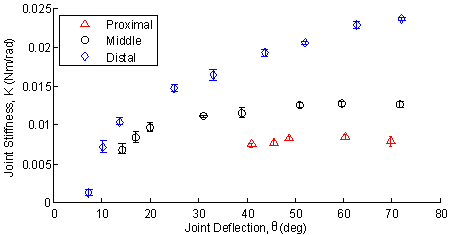
\includegraphics[width=.7\textwidth]{chap1img/jointDeflection4.pdf}
      \caption[Joint stiffness as a function of deflection]{Joint stiffness as a function of deflection. Values are calculated using the mean joint deflections reported in Table \ref{tab:deflect}. Error bars show the range of K values possible with all permutations of $\pm\sigma$ in joint deflection. Stiffness is nonlinearly related to deflection and increases as the toe deflects further.}
      \label{fig:jointDeflect}
   \end{figure}

\subsection{Subsection Title} %level 3
Text  
\chapter{Background and related works}
\label{chap:bg}
% This chapter will cover: Effect of preprocessing. SPM smoothing, Random field
% theory for enforcing smoothing.

% a very high level overview.
The human brain is organized into distributed functional modules that work
independently but also interact with one another during cognitive
activity. There appears two principles of how the brain function is organized:
functional integration and functional
specialization~\cite{friston2007statistical}. Functional specialization assumes
the modules that process a particular cognitive activity can be localized to an
anatomical region in the brain. In functional specialization, one studies the
relationship of specific anatomical regions and cognitive activity. However, the
brain regions or functional modules do not work alone. They interact with each
other in a complex and dynamic way. Functional integration focuses on such
interactions.

% what will be covered in this chapter.
This chapter provides background information about the current research
exploring brain's functional network using rs-fMRI. I will begin with the
relationship between brain activity and fMRI, and give the definitions of
functional connectivity and functional network. Then I will survey various
classes of methods for estimating functional connectivity and networks.

%% Brain network organization, anatomical/functional connectivity, fmri BOLD,
%% oxygen, task, resting-state, functional network
\section{Resting-state functional networks}
% the interaction: anatomical connectivity and functional connectivity. 
The interactions among various functional modules of the brain can be
represented by the connectivity among anatomical regions. Two sets of MRI
techniques are widely used for mapping the \emph{in vivo} connectivity of the
human brain. Diffusion MRI, or more specifically, diffusion tensor imaging
(DTI), as a structural imaging technique, detects the anisotropy of the neural
axons in the brain's white matter by measuring the diffusion of water
molecules. Such anisotropy is used for identifying the anatomical connectivities
between two regions in the brain's white
matter~\cite{jirsa2007handbook}. Functional MRI (fMRI) imaging, in contrast,
serves to explore the functional links between two regions of interest in
brain's gray matter. The functional connections are the actual flow of
information through the anatomical links represented by the DTI. Researchers
have demonstrated the correlation between the anatomical and functional
connections. Such correlation is an indication that functional connectivity is
physically constrained and modulated by the structural
connectivity~\cite{honey2009predicting}. However, functional and structural
connectivity are not exactly equal, suggesting the dynamic characteristics of
the functional patterns depend on the brain's state. The work in this dissertation
is focused on functional connectivity.

% fmri intro, BOLD, oxygen, task-based. 
Information is transferred in axons between neurons by the release of
neurotransmitter molecules at synapses. The interactions between
neurotransmitter and receptors consume energy. Because energy is produced by
oxidative metabolism, increased synaptic activity will also increase local
demand for delivery of oxygen. This, counter intuitively, increase the local
blood flow, and increases the $T_2^*$ image
intensity~\cite{lewin2003functional,stroman2011essentials}. Even deoxygenated
hemoglobin decreases during neural activity, MR signal increases. This is
because more oxygen is supplied to the brain region than is consumed.

Haemoglobin have different magnetic property when it is bound to oxygen. This
changes the local distortions of a magnetic field, which can be detected by MRI
scanner. The relaxation times depends on the level of blood oxygenation, and the
MRI signal depends on the relaxation time, and is called blood oxygenation
level-dependent (BOLD) signal.

To understand the response of BOLD signal to a general stimulus signal, we need
to know its response to a very short impulse signal, namely, a $\delta$
function. It is noted that the BOLD signal have about two seconds lags after the
onset of stimulus. This initial dip is attributed to the transient increase of
deoxygenated hemoglobin. After 4 to 6 seconds, the demand due to increase neuro
activity results in an increased inflow of oxygenated blood, and it reaches the
highest point. After the neuro activity stops, the BOLD goes below the baseline
level. It takes about twenty seconds for the BOLD to go back to the baseline in this
\emph{poststimulus undershot}. The balloon model \cite{buxton1998dynamics} is
used to explain this extended period. The response function to a $\delta$
function is called the Hemodynamic response function (HRF). The response of a
general boxcar function, would be the convolution of the boxcar function and the
HRF.

Because the resolution of fMRI is much higher than the single cell or neuron,
the BOLD signal reflects the energy demands of neuropopulation that fire
together with a common functional purpose~\cite{huettel2004functional,
  jezzard2003functional}. Besides fMRI, other techniques are also used for
mapping the functions of the brain. They differ in terms of both their temporal
and spatial resolution. In general, electrophysiological methods, such as
electroencephalography (EEG) or the associated magnetic version
magnetoencephalography (MEG), record the neural events in real time; hence,
these methods have relatively high temporal resolution. On the other hand, fMRI
and positron emission tomography (PET) detect the change of blood flow due to
neuronal information processing, and have high spatial resolution (1-5 mm), but
lower temporal resolution because of the delayed haemodynamic changes.

% functional connectivity and functional network.
fMRI was initially discovered as a tool to map the brain's activity for subjects
in specific cognitive experiments. One compares the BOLD signal at a specific
region in the brain with the paradigm task signal. Because of the nature of the
haemodynamics of the blood, the paradigm task signal is the convolution of the
original paradigm function (for example, a boxcar function) with the
haemodynamic response function (HRF). Later, researchers found that the BOLD
signals can be used not only to detect the functional patterns in
stimulus-guided experiments, but also to explore the co-activation of the brain
when the subjects are not performing cognitive
tasks~\cite{biswal1995functional}. In such experiments, the primary goal is to
identify the functional connectivity between pairs of regions in the
brain. Functional connectivity is defined as the temporal dependence of neuronal
activity patterns of spatially remote (or anatomically separated) brain
regions~\cite{friston1994functional, worsley_analysis_1995,
  friston1994analysis}. The temporal dependence is typically measured by the
linear correlation across all time points. Although the temporal correlation
within the BOLD signal of a single region or voxel violates the independence
assumption of the time point samples, this temporal correlation is often safely
ignored. Alternatively, one can also identify functional connectivity by
transforming the signals into the frequency domain and using the coherence of
two signals at a certain frequency band. The coherence as similarity measurement
is equivalent to band pass filtering the original BOLD signal and computing the
linear correlation~\cite{cordes2000mapping, cordes2001frequencies}.

% Define a functional network. 
The pairwise correlation or coherence only measure the functional connectivity
between regions as a local measurement. As the whole brain is organized as a
complex system with many such pairwise interactions, it is of interest to find
out those regions with similar patterns of neuronal activity. A functional
network, or functional system (hereafter used interchangeably), is a collection
of separate anatomical regions that have similar patterns of activity measured
by BOLD signal. The regions within a functional system may have direct or
indirect information flow among them. Together the system serves one or more
cognitive tasks. An anatomical region may participate in different functional
systems during different cognitive tasks.

%% [ Various levels. Task, resting, Cognitive disease. Mental disorder. Low
%% frequency. Correlation.
The correlated fluctuation of multiple brain regions not only occurs in
stimulus-evoked experiments, but also in experiments where the participants rest
passively without any cognitive activity. Therefore, the resting-state fMRI
(rs-fMRI) becomes a powerful tool for probing such intrinsic activity in a
resting brain~\cite{raichle2001, fox2007spontaneous}. The original name of the
rs-fMRI is not accurate, since the brain is not truly in a resting state even
without any cognitive activity. The resting brain consumes about 20 percent of
the energy of the whole body, but it occupies about only 5 percent of the body
mass~\cite{fox2005human}. The study of the functional organization of the
resting brain provides new insights into how functional connectivity relates to
cognitive psychology and neurodegenerative diseases.  Because the pathologic
conditions appear to be reflected by the interactions within or between the
functional systems, the rs-fMRI study also holds valuable diagnostic and
prognostic information towards various neurological or psychiatric diseases
including Alzheimer's diseases, depression, and
schizophrenia~\cite{fox2007spontaneous, greicius2007resting,
  greicius2003functional}, etc. The reason for this spontaneous activity is
largely unknown, although some researchers reasonably postulate that it is a
predictive intrinsic response to the unknown events in the outside
environment~\cite{deco2010emerging}.

% preprocessing. motion correction. global signal regression? slice timing
% correction, nuisance parameter regression (GM, WM, CSF), registration.
\section{Preprocessing fMRI data}
Due to the noise and artifacts in fMRI data, multiple preprocessing steps are
typically taken before the real analysis starts. The preprocessing steps include
motion correction, slice timing correction, spatial and temporal filtering,
registration between structural images and functional images, registration
to the standard template, and removing physiological noise, etc.

Because of a subject's head movements during the scan, the volumes at various
time points are usually not perfectly aligned. A rigid body registration is
usually done between the volumes at different time points, with either the first
volume or the middle volume as a reference. This is called motion
correction. After correction, the same voxel coordinate is assumed to map to the
same brain structure across all time points, although the correction is often
not perfect. The motion correction parameters of each volume are often used as
independent variables for a regression in order to remove the motion effect. The
first few time points are usually discarded in case the scanner is not in a
stationary state.

Slice timing correction is needed because each slice of fMRI volume is not
scanned at the same time. Figure \ref{fig:slicetiming} shows the shifted time of
scans for different slices and the method of interpolation.  The shifted time
will give suboptimal experiment results during the analysis, especially for the
event-based experiments. One typically uses an interpolation step to obtain a
volume in which all slices are at the same time point. Care must be taken for
the ordering of the slices as the ordering is scanner dependent.


Because of the physiological process of the BOLD signal, most of the interesting
information is concentrated at the low frequency range of the signal (0.01 --
0.1 Hz). The temporal band-pass filter is usually applied to remove the very low
frequency (below 0.01 Hz) and higher frequency (above 0.1 Hz). Also, due to the
spatial process of fMRI data acquisition, neighboring voxels typically have
similar signal patterns. The statistical parametric mapping
method~\cite{friston2007statistical} makes use of this spatial dependency by
applying a spatial Gaussian filter, and further enforces the smoothness of the
signal on the spatial domain. This filtering increases the SNR, but inevitably
discards finer patterns with size smaller than the smoothing kernel. Chapter
\ref{chap:method1} and Chapter \ref{chap:method2} will discuss more principal
methods that model this spatial dependency with no spatial smoothing, or very
small, conservative smoothing.

In order to report the experiment results in a standard way such that others can
understand, the structural images and functional images are both registered to a
standard template, such as the MNI 152
template~\footnote{http://www.bic.mni.mcgill.ca/ServicesAtlases/ICBM152NLin2009}. The
functional images are first registered to structural images of the same subject
by a rigid body transformation. The structural images are then transformed to
the standard template by affine transformation. Because of the plasticity of the
brain anatomy, the registration of the subject's structural image may need
nonlinear transformation to register to the
template~\cite{jenkinson2012fsl}. After the structural images are registered to
the template, the functional images will also be brought to the template space
by the same transformation. The last step is the nuisance parameter
regression. The nuisance parameters include the six motion correction parameters
that are estimated in the previous motion correction step, and also the mean
signal of the white matter and cerebrospinal fluid (CSF). The motion correction
parameters are taken into account because even though the fMRI data are motion
corrected at the first step of preprocessing, the motion may still have an
impact on the estimation of the general linear model (GLM) of task-based fMRI,
or the correlation for the rs-fMRI. The mean of white matter and CSF is
regressed out as these average signals are assumed to consist of physiological
noise. Since there is no information of the physiological signal such as heart
beating and breathing, the mean of white matter and CSF is used as surrogates
for such confounding signals.

With completion of the above preprocessing steps, the data are ready for
analysis. The above preprocessing steps may vary depending on the specific
experiments. For example, the slice timing shifting is not a severe issue for
rs-fMRI analysis and can be skipped. Besides, the preprocessing steps may not
have consistent impact on the fMRI processing pipeline. For example,
Zhang~\cite{zhang2009evaluation} pointed out that slice timing correction and
global intensity normalization have little consistent impact, but spatial
smoothing, temporal detrending, high-pass filtering and motion correction
significantly improve the pipeline performance across all subjects.

\section{Related methods}
The temporal dependence of the spatial regions can be represented in multiple
ways. Depending on whether one is interested in a specific region or a full brain's
functional patterns, one can select the  seed-based method or the full brain
method. For the class of full brain methods, there are methods that
define the region of interest (ROIs) and build a functional network by
estimating the edges of the graph with nodes defined by the ROIs. Also, the
parcellation defines an image segmentation problem where the regions with higher
functional connectivities are grouped into a single cluster. In this section, I
will give a short survey of the various methods, show their advantages and
disadvantages, and the similarities and differences with our methods.

\subsection{Seed-based methods}
Depending on the specific experiment goal, functional networks may be
represented in various ways. A straightforward yet statistically powerful method
is to compute the linear correlation between \emph{a priori} given seed regions and
all other regions in the brain~\cite{biswal1995functional, buckner2008brain,
  buckner2009cortical}. The correlation values are typically Fisher transformed
in order to meet the normal distribution assumption in the following hypothesis
test. Those transformed correlation values with $p$ value less than a certain
threshold are regarded as the existence of the functional connectivity. All
voxels or regions that are functionally connected to the seed regions belong to
the same functional system. The seed-based methods are useful when a user asks a
straightforward question and knows what functional system is of interest. The
result is easy to interpret compared to other more complex methods.  The
advantage of seed-based methods is their simplicity and relatively ease of
extention to multiple subjects. A user simply computes the average correlations
across subjects for a given pair of regions. When users are interested in the
connectivity to multiple regions, they can define more than one seed.

However, this method has a limitation: the user has to know the location of the
seed in advance. The seed as \emph{a priori} information is an advantage when it
accurately represents the functional patterns of interests. However, a
functional system cannot be identified if the seed region falls out of the
system.  Despite this limitation, researchers frequently use this method,
sometimes with better visualization by dynamically moving the seed and showing
the real-time functional system associated with the current seed
region~\cite{yeo2011organization}.

\subsection{ICA and other decomposition methods}
Because functional networks are in a large scale over the whole brain, and in
a distributed manner, a multivariate analysis is a better way to explore the
full brain's functional organization. A large class of multivariate methods
use the signal-decomposition concept from the signal processing community and
decompose the BOLD signal at each region or voxel into various independent
components, each of which is part of one functional system. The signal and the
weight coefficients of these independent signals represent how much of the
current voxel belongs to certain functional network component. One widely
accepted method in this class is the independent component analysis (ICA). ICA
was originally introduced in the signal processing field to separate various
sources of signals from samples of mixed signals and later was applied to
rc-fMRI data~\cite{nggroup2012, beckmann2005tensorial,
  damoiseaux2006consistent}. The central limit theorem states that the sum of
two independent signals is more like Gaussian, than any of the original
signals. Therefore, maximizing the non-Gaussianity gives us the original
independent components. Besides the maximization of non-Gaussianity, the
independent components can also be estimated by minimization of mutual
information, or by maximum likelihood~\cite{hyvarinen2000independent}.

There are two varieties of ICA method when applying to rs-fMRI dataset. Spatial
ICA assumes all the voxel intensities at a certain time point as one mixed signal
sample. Therefore, the mixed signals are independent across all spatial
voxels. Alternatively, temporal ICA treats each BOLD time series at a voxel as a
mixed signal; hence the source signals are independent across the time
point~\cite{calhoun2001spatial}. Notice the functional map we are interested in
is the rows of source signal matrix $S$ for spatial ICA, and is the weight
coefficients matrix $\tilde A$ for temporal ICA (see Figure \ref{fig:c2ica} for
an illustration). Because of the large number of voxels compared to the number of
time points, the spatial ICA is typically used for rs-fMRI analysis. Compared to
seed-based methods, ICA is purely data-driven, and can identify networks over
the whole brain, including the already well-known cognitive processing systems
such as motor~\cite{biswal1995functional},
visual~\cite{damoiseaux2006consistent}, attention~\cite{fox2006spontaneous}
executive control and salience network~\cite{seeley2007dissociable,
  seeley2009neurodegenerative}.

However, because ICA needs to estimate both the independent components and
mixing coefficients, it is a significantly more difficult task. Before applying
ICA, the data usually needs a whitening step with principal component analysis,
and is thus rotated such that it has unit variance in terms of the covariance
matrix, which greatly simplifies the ICA problem. The estimated independent
components are usually $z$ transformed and thresholded for visualization
purpose. Because the resting-state brain functional patterns are unpredictable,
the output independent components need to be visually inspected in order to
identify physiologically meaningful components. The iterative optimization also
introduces variability between multiple runs of ICA with different initial
states. In addition, the dimensionality in the preprocessing step of principal
component analysis (PCA) is typically chosen arbitrarily, adding more variation
in the results. A recent test on the reliability of ICA~\cite{zuo2010reliable}
shows how the choice of the dimension and the number of components have an
impact on the consistency of the results.

\subsection{Segmentation-based methods}
The functional networks estimated from ICA are represented by continuous numbers
and have to be normalized to the $z$ score and thresholded to give a binary
map. The thresholding adds ambiguity to the consistency of the results. An
alternative class of methods formulate the problem of identifying functional
patterns as an image segmentation problem. The image segmentation problem can be
also viewed as a data clustering problem in general data mining. However, since
the data points are indeed voxels in the fMRI images, the spatial context
information is also useful for the clustering. Therefore, we name this class of
methods as image segmentation, to indicate the possible usage of spatial
information. Once the fMRI images are segmented into various disjoint sets of
regions, the voxels in the same regions have a higher correlation, and hence are
believed to be functionally connected. Compared to ICA, the segmentation problem
typically has a binary map for each functional network, i.e., the clusters,
although some soft segmentation methods exist. The methods used for segmentation
include hierarchical clustering~\cite{salvador2005neurophysiological,
  cohen2008defining, cordes2002hierarchical, bellec2010multi}, partitioning
clustering~\cite{bellec2010multi} and spectral clustering
~\cite{van2008normalized, craddock2012whole}. The early works of fMRI image
segmentation~\cite{cordes2002hierarchical} are limited to a few slices due to
the computation cost. Even within a few slices, the segmentation method is still
able to identify the major functional components, and they shows that the
results are robust to the confounds due to the subject motion and physiological
noise. One interesting property of the hierarchical clustering technique is the
potential of detecting the hierarchy of the brain's functional
organization. Since the brain's functional patterns are widely believed to be
also hierarchical~\cite{yeo2011organization}, a computational method will be
very useful if it can naturally identify the subclusters within a certain
cluster. Notice that the hierarchical clustering method is different from the
\emph{hierarchical MRF} method in the following chapter. The former builds a
hierarchy on the clusters, whereas our method builds the hierarchy on the group
and subjects' functional network maps.

Among the segmentation methods, Mezer et al.~\cite{mezer2009cluster} use the
windowed Fourier transform and the spectrum below 0.2 Hz on the frequency
domain, as well as the BOLD time series in the original image domain as features
for the K-Means clustering. To test if the clusters estimated by K-Means are
significantly different, they used a repeated measure ANOVA test between each
pair of clusters. The experiments in Mezer's work showed strong links between
the functional patterns and the tissue architecture, suggesting the possibility
that the rs-fMRI signal may include the contributions from physiological and
artifact noise factors that cannot be easily separated. In Figure
\ref{fig:coherence}, we did a simple experiment for using spectral coherence as
the similarity measure and use spectral methods for segmentation. From the
figure, we can identify the visual area (the green) and the functional regions
at temporal lobes (blue). Since we define each voxel as a node on the graph, the
total number of data points is big, and the computation of the similarity matrix
takes long time. The example here uses only 10 $z$ slices for illustration.

To decide the number of clusters in the functional network map is a difficult
problem of model selection. Most of the methods use seven clusters, since the
clustering into seven networks has a good match with the existing cognitive network
configuration~\cite{yeo2011organization}. Other choices are possible if the goal
is to identify the functional patterns at a finer scale. Another reason of
choosing large number of clusters is to have a finer parcellation in the local
scale. In a local parcellation, only the locally coherent functional regions are
grouped into the same cluster. The remote functional regions may not be grouped
into the same cluster eventhough they belong to the same functional
network~\cite{mezer2009cluster}. Such a local grouping approach is similar to the
super-pixel approach widely used in the computer vision
community~\cite{levinshtein2009turbopixels, achanta2012slic}, where researchers
group similar pixels into small regions as a preprocessing step for higher-level
vision analysis. The grouping procedure is conservative in that only the
spatially neighboring pixels are grouped. The super-pixels are used for the
higher level image understanding problem in order to save computation time. One
example of such functional network parcellation is
Thiron~\cite{thirion2006dealing}, where the primary goal is to find spatially
coherent clusters that are connected. Therefore, the spatially remote regions
cannot be classified into the same cluster. The advantage of such parcellations
is the small regions modeled as groups of voxels better represent true regions
of activity in task-based fMRI data, and are less sensitive to the
misregistration across subjects. The parcellation also reduces the multiple
comparison problem that is typically found in the statistical parametric mapping
method. Thiron et al. uses a spectral clustering approach with multidimensional
scaling (MDS) representation of the dataset, and the C-Means method for
clustering. The method is able to estimate a spatial coherent group clustering
from the subject parcellations. Another example of finer parcellation is found
in Craddock et al.~\cite{craddock2012whole}. The goal of their work is to
evaluate the suitability of a few parcellation schemes on a group of subjects'
rs-fMRI data. The authors use the normalized cut method~\cite{shi2000normalized}
to segment the brain into a large number of spatial and functional homogeneous
regions. A graph is defined by adding edges only between spatial neighbors, with
the weights on the edges defined by the linear correlation between BOLD
signals. This definition of edges and weights means the functionally homogeneous
voxels may be in different clusters if they are not spatially adjacent. Since
the number of clusters in their experiments is relatively large (50 - 400), the
estimated parcellation map will not be easily interpreted as functional
networks, but will be used for further analysis. For group parcellation,
Craddock et al. use second-level group clustering similar to the work of Van
den Heuvel~\cite{van2008normalized}. The estimated adjacency matrix estimated
from subject parcellation was averaged across subjects, and the average matrix
was used for a second-level normalized cut algorithm.


The segmentation of functional network is not necessarily limited on rs-fMRI
data. It can also be used for the task-based fMRI. The work of Michel et
al~\cite{michel2012supervised} is one example in this range. Michel et al. use a
generalized hierarchical clustering based on the Ward algorithm to build a tree
of hierarchical clusters. The leaves of the tree are individual voxels, and the
root includes all voxels. The authors compute the optimal pruning of the tree by
fitting the average signals of the leaves at each pruning depth to a general
linear model. The clusters of optimal trees are able to predict the behavior
variables. Varoquaux et al. from the same research group use the methods of
Michel et al.~\cite{michel2012supervised} for solving an active region
detection problem of task-based fMRI data~\cite{varoquaux2012small}. Whereas the
goal of Michel et al. is to identify the functional network patterns using the
supervised clustering method with clinical variables, the goal of Varoquaux et
al.~\cite{varoquaux2012small} is to detect active regions when the
observation is small and the number of predictors is large. By grouping
spatially adjacent voxels with similar BOLD signals into clusters and using the
clusters as the independent variables, varoquaux et al. solve the problem of
large number of predictors, and are able to identify the functional patterns when
there are more voxels than the number of observations.


Some of the methods we proposed in Chapters \ref{chap:method2} and
\ref{chap:method3} belong to the class of segmentation. However, we defined the
additional structures based on the spatial context information, and the
intersubject coherence assumption, so the model is more complex than the above
works, and therefore requires more advanced statistical inference methods.

\subsection{Methods based on graph theory}
Functional networks can also be represented by graph~\cite{bullmore2009complex,
  achard2006resilient, sporns2004organization}. Our improved understanding of
the complex systems and the increasing availability of large datasets of systems
have led to the insight that these complex systems share similar behaviors that
can be represented by the same parameters~\cite{bullmore2009complex}. To build
an abstract graph from the fMRI data, one typically chooses some ROIs as the
node of the graph, and estimates the existence or lack of edges between the
nodes. The signal on each node is computed by averaging the BOLD signals of all
the voxels within a certain radius of the ROI, usually a few millimeters (see
Figure ~\ref{fig:brain_graph} for an illustration). The edge is estimated by
computing the linear correlation or the frequency coherence between two
ROIs. Once the functional network is represented by a graph, a rich class of
methods in graph theory can be used to explore the global property of the
graph. For example, the high degree of a node indicates its role as a hub in the
network, and the distribution of the degrees is used to explore the
vulnerability of the graph when some \emph{hubs} are removed from the
network. Various measures of the network topology are estimated from the graph
to explore the similarities and differences between the functional network of
the brain and other complex networks such as social networks and wireless
networks. The graph property can also be used to explore how the functional
system is configured to allow maximum flow of information with minimal
wiring. For example, the \emph{small-worldness} attribute is shared by many
real-world networks including the functional networks of the human brain, and it is
hypothesized that the small-worldness is chosen by evolution for high efficiency
of information transfer between nodes at low connection
cost~\cite{achard2006resilient, bullmore2009complex, bullmore2012economy}.

The network estimation results depend on how we define the nodes of the
graph. Nodes should be defined as  brain regions with homogeneous functional
and anatomical patterns. The comparison of functional and structural networks is
meaningful only when they share the same definition of graph
nodes~\cite{rubinov2010complex}. Due to the limits on the available methods and
the computation resources of estimating networks with continuous edge weights,
typically one constructs a binary network by thresholding the similarity
matrix. How to choose the optimal thresholding parameter is an open
question. More importantly, there is no principal method for combing the
networks from a group of subjects.

\subsection{Group analysis}
%% [Group of subjects. Variation and shared information. resting-state intrinsic
%% cognition. 1000 connectomes. ]

The analysis fMRI data is challenging, due to the scanner noise, physiological
noise such as blood vessel and heart beat, and subject's head motion. Sometimes
subjects have random thoughts even when specifically instructed not to think of 
anything  during the data acquisition. The functional connectivity and
network estimation is still not accurate and consistent even when various
preprocessing techniques are used. On the other hand, because rs-fMRI
experiments have much lower requirements for the patient subjects or control
subjects compared to paradigm design experiments, it is possible to collect the
rs-fMRI data from a big group of subjects. The functional networks detected by
either model-based methods such as seed-based correlation, or data-driven
methods such as ICA, are highly reproducible across participants and scans. The
more accurate and consistent functional networks can be estimated by using the
statistical power of the group analysis. With the initiative of 1000 Functional
Connectomes Project, a large cohort of data are available for researchers to
explore the relationship of functional networks to the subjects' age, gender, etc.

% seed-based methods extend to grp analysis.
Compared with single-subject analysis, the methods for multiple-subject
functional network analysis are not yet established. The seed-based methods
typically compute the correlation or regression coefficients between regions
independently for each subject. The correlations or regression coefficients are
treated as a statistic of each subject and go into a second-level
analysis. The second level can be either fixed-effect analysis or a
random-effect analysis with a standard hypothesis testing. The population-based
z-score maps have to be corrected for multiple comparisons~\cite{fox2005human}.

% group ICA
Group ICA is used as an extension of single-subject ICA in order to seek a set
of independent components shared across multiple
subjects~\cite{calhoun2001spatial}. In a typical group ICA study, all subjects
are registered to a common atlas and are assumed to share a common spatial
component map but have distinct time courses. The BOLD signals from all subjects
are concatenated temporally, followed by a single-subject ICA. The subject
component maps are then obtained by a back-reconstruction procedure.

Alternatively, a single-subject ICA is applied on each subject first, and a
group summary is estimated from the estimates of subject functional
patterns. Some methods that we have introduced such as the segmentation-based
approach~\cite{bellec2010multi,craddock2012whole} are in this range. If the ICA
is used for estimating the spatial patterns at the subject level, it is not
straightforward to conglomerate the spatial maps of multiple subjects and derive
an optimal set of group maps. Such difficulty of matching the network label maps
is because the component maps of subjects are not perfectly aligned with each
other, and it is difficult to find the correspondence between subject A's
component $i$ and subject B's component $j$. To solve this problem, Esposito et
al.~\cite{esposito2005independent} propose a \emph{self-organizing} method for
the group map estimation. A series of spatial component maps are estimated by
the regular ICA method for each subject, and these maps are all put in a single
pool. The similarity between each pair of component maps in this pool is defined
and calculated. Then, Esposito et al.  did a clustering on the pool of component
maps. The cluster center of the maps is believed to be the group component
map. Neither of the above approaches iteratively refines group (or subject) maps
once the subject (or group) maps are estimated.

Varoquaux et al.~\cite{varoquaux2010group} give an extension of ICA method for
group analysis. The authors define a generative model, in which the subject
component maps are assumed to be generated from a group component map. In
particular, the subject map is a weighted group map with an additive noise
term, and the observed BOLD signal of each subject is a linear combination of
the subject's components with additive noise. The estimation takes two
steps. At the subject level, each subject's data are decomposed by principal
component analysis (PCA) and an estimate of the subject component map is
obtained. At group level, the authors use canonical correlation analysis (CCA)
to find a common subspace among the estimated subject component maps. Such an
approach is in the class of \emph{bottom-up} methods that we introduced in
Figure \ref{fig:bidirections}, since the group component map estimate is not
used to iteratively refine the subject estimation. Besides, there seems to be
a discrepancy between the group map definition and estimation. That is, the
author~\cite{varoquaux2010group} did not provide any justification for CCA
giving an optimal estimate of the generate model defined on the group level.

Another interesting study by Varoquaux et al.~\cite{varoquaux2011multi} uses
dictionary learning for the group analysis. Dictionary learning is in the class
of linear signal decomposition, with ICA as a special case. In this work, the
authors again defined a generative model, where the observed subject data matrix
is the product of the loading matrix (i.e., the weighting coefficients) and a
signal matrix (also called the code in the dictionary). The loading matrix is
the subject-specific spatial map, and is generated from a population spatial map
with an additive noise term. The objective function can be written as a
nonhierarchical form, and is a function of the subject component map and
group component map. The optimization is done by a coordinate descent
approach. Overall, the model is similar to what we will propose in Chapter
\ref{chap:method3} in that a hierarchical map is defined and estimated. In
addition, it is different from previous work~\cite{varoquaux2010group} as the
group and subject maps are estimated iteratively in the coordinate descent
framework. So, the Varoquaux et al. method is indeed a counterpart to our
hierarchical Markov random field model, but in the linear signal decomposition
fields.

% talk about tensor ICA, and the tensor decomposition method such as
% multi-linear...

% assumption of the group study. challenges of group study.
Despite the promising future of using large populations for studying the
functional network and its relationship to the underlining structural patten,
the group study also poses new challenges when putting all datasets
together. The folding patterns of the cortical surface, and the structure and
size of brain regions, are all different across individual subjects. Because of
such structural variation, the intersubject registration is often not accurate
enough to map the same anatomical structures to the same coordinates in standard
space. Such inaccurate registration may be due to the imperfect coregistration
algorithm itself, or due to the difference of individual subjects' cortical
structures. Even if the anatomical structures are aligned among multiple subjects,
the functional patterns of each subject are not the same. Although numerous
studies have shown the relationship of the functional connectivity is related to
the structural connectivity~\cite{honey2009predicting,hermundstad2013structural,
  honey2007network}, it is less well known how and to what extent this
relationship is reflected by the variation of functional connectivity.

\subsection{MRF and spatial constraints}
%% \cite{michel2012supervised} spatial constrained clustering. and other papers
%% in this group.

% Below need to add reference of SPM, and the random field model of Worsley.
Because of the univariate characteristic of the statistic parametric mapping
(SPM)~\cite{friston2007statistical} method, the spatial context information is
not taken into account in the model. That is, if one arbitrarily permutes the
location of the voxels in the brain, the resultant activation map in a
task-based experiment does not change, i.e., the original activated voxels are
still activated. To take the spatial information into account, one typically
forces the spatial homogeneity by applying a Gaussian filter on the spatial
domain as a preprocessing step. The filter increases the signal-to-noise (SNR)
ratio but inevitably has a blurring effect that sometimes results in the loss of
finer structures of the functional patterns.

Markov random field (MRF), as a principal method of modeling spatial context,
 has been brought into image processing fields by
Geman~\cite{geman1984stochastic}. The first application of MRF to fMRI analysis
was by Descombes et al.~\cite{descombes_spatio-temporal_1998}. Although this is
an early work of MRF's application, I give some details of their work because of
its novelty. In their work, the authors propose to use MRF for two
purposes. First, they used a spatiotemporal MRF to restore the noisy BOLD
signal instead of a general temporal filter and spatial Gaussian filter. Second,
they compared the restored BOLD signal with the stimulus haemodynamic response
function for detecting the activation map, which is modeled by a spatial
MRF. For the first goal of BOLD signal restoration, the authors defined a graph,
whose nodes or voxels have 12 neighbors: 8 as spatial neighbors, and 4 as
temporal neighbors. A hidden continuous variable was defined at each node of
each time point to represent the true BOLD signal's intensity. To preserve the
discontinuity, another line process MRF was defined on the dual lattice to model
the existence or lack of edge between spatial neighbors. The statistical
inference of this spatiotemporal MRF is solved by simulated annealing (SA). For
activity detection, a second MRF was defined on the activation variables, and
the MRF included only spatial neighbors. Although the work was applied on the
fMRI data in paradigm design, the concept of spatial regularization and Bayesian
method is also applicable to the rs-fMRI data.

Another early work of Hartvig et al.~\cite{hartvig2000spatial} aims at using the
spatial context information for activation detection of task-based fMRI
experiments. The authors' inductive bias is that the activation region should
not be too big or to small. According to this assumption, they define a hidden
activation variable taking value in $\{-1, 0, 1\}$ to represent negative-active,
no-activation, and activation state. In addition, the estimated activation
coefficients from the standard SPM are assumed to be Gaussian given the hidden
variable is no-activation, and Gamma distribution given the hidden variable is
activated. The prior distribution of a small set of neighboring voxels' hidden
variables is defined to reflect the inductive bias, and the goal is to estimate
the posterior of the hidden activation variable given the observed activation
coefficients from SPM. The Hartvig et al. model is not MRF strictly speaking,
although the model represents the authors' assumption of the spatial context.

A recent work of application of MRF to task-based fMRI data is by Ou et
al.~\cite{ou2010combining}. In their work, the authors define a MRF on the
activation variables, and the MRF prior favors spatially coherent activated
regions. The conditional probability of the observed data is defined by a
general linear model (GLM) with the hidden activation variables as
parameters. One important characteristic of the work of Ou is the parameter
estimation, including both the GLM's parameter and the MRF's parameter. The
authors define the MRF prior such that the samples drawn from the prior agree
with the spatial properties of the true activation map in fMRI
experiments. Therefore, they use the frequency counts to set the pairwise
potentials with an additional parameter to control the overall
\emph{sharpness} of the joint component of the prior. This method is similar
to the work of Boykov et al.~\cite{boykov2001interactive} and Rother et
al.~\cite{rother2004grabcut}, where a parameter is estimated from the data by
counting over the whole image. The additional parameter is also estimated from
the data in simulated experiments. The method of Ou is for single
subjects.

Penny et al.~\cite{penny2005bayesian} define a MRF on the regression
coefficients of the general linear model on a task-based experiment. Because the
regression coefficients are continuous, the authors model the prior distribution
by the multivariate Gaussian distribution, with the precision matrix represented by
a Laplacian operator. This Laplacian operator penalizes differences between
the coefficients of neighboring voxels. In the generative model, the sample of this
prior distribution can be generated by first draw independent samples from
Gaussian, and then applying the Laplacian operator mapping.

Overall, the methods of functional network estimations have been ranged from the
basic seed-based approach to more advanced multivariate, full brain analysis,
and from single-subject analysis, to a pooled summary of multiple subject
analysis, to the more complex joint analysis of both population and
individuals. In the following chapters, we will introduce our contribution to the
methods by combining MRF and a hierarchical model. It should be noted that the
more complex method will achieve better results only when the model fits the
data well, and the statistical inference will successfully find the optimum or
reasonably approximate the optimum solution.



\begin{figure}[p]
  \centering
  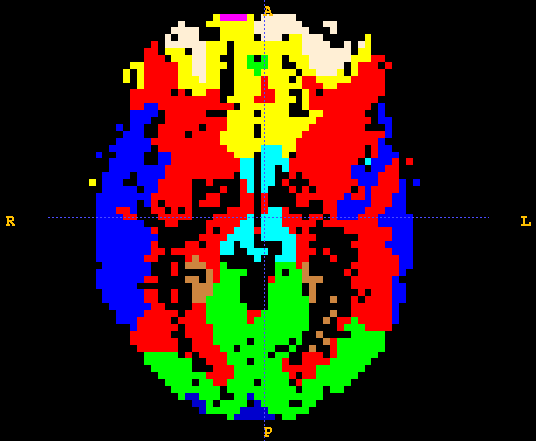
\includegraphics[width=0.3\textwidth]{figures/math/coherence/a}
  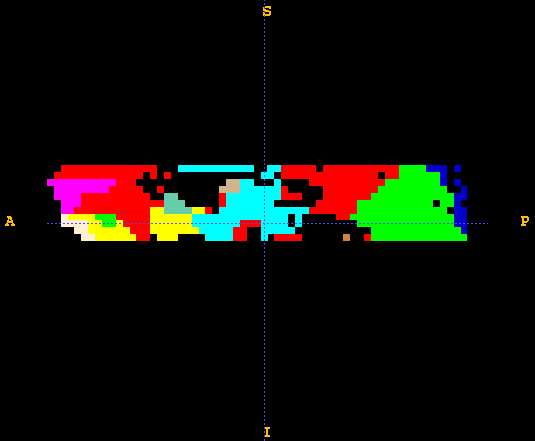
\includegraphics[width=0.3\textwidth]{figures/math/coherence/s}
  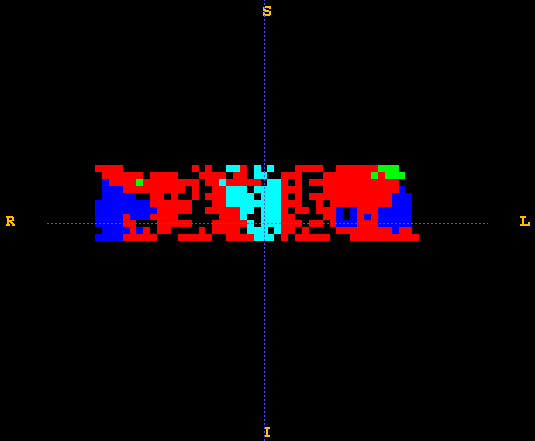
\includegraphics[width=0.3\textwidth]{figures/math/coherence/c}
  \caption{Segmentation map of a rs-fMRI volume. The spectral coherence between
    0.01 to 0.1 Hz is used for similarity between pairs of voxels. A spectral
    clustering method~\cite{von2007tutorial} is used for dimension reduction
    followed by a K-Means clustering. We choose 12 clusters and 10 slices on $z$
    direction to save computation time. }
  \label{fig:coherence}
\end{figure}

\begin{figure}[ptb]
  \centering
  \includegraphics[width=0.9\textwidth]{figures/c2/brain_graph}
  \caption{Using a graph to represent functional networks. A series of ROIs are chosen
    based on what questions  asked. Tthe signal at each ROI is computed by
    averaging the BOLD signals of all voxels within the sphere. The edge
    of the graph is estimated using the similarity of the signals between the
    ROIs. }
  \label{fig:brain_graph}
\end{figure}

\begin{figure}[ptb]
  \centering
  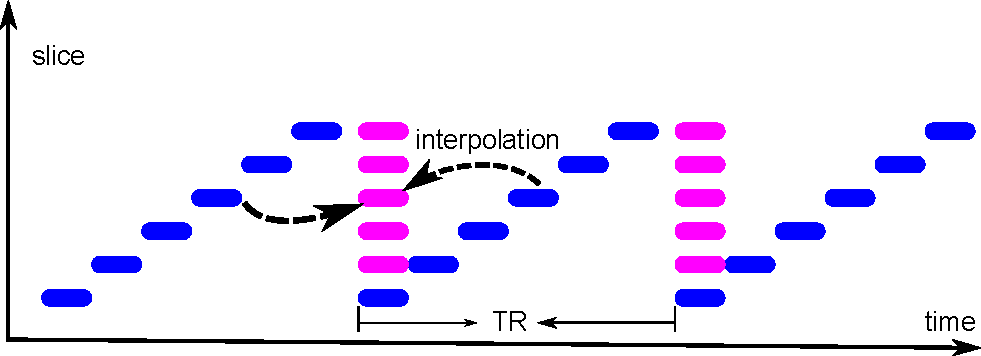
\includegraphics[width=0.9\textwidth]{figures/c2/slicetiming}
  \caption{Slice timing correction. The data at temporally adjacent slices are
    resampled and interpolated to obtain a data point at the same time with the
    reference slices.}
  \label{fig:slicetiming}
\end{figure}

\begin{figure}[ptb]
  \centering
  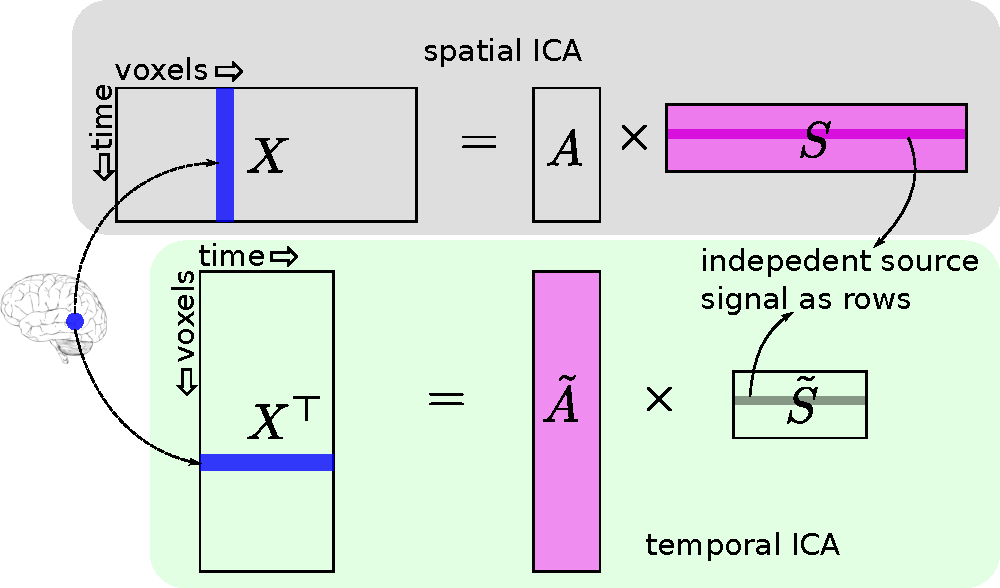
\includegraphics[width=0.8\textwidth]{figures/c2/ica}
  \caption{Spatial ICA versus temporal ICA for BOLD series of length $T$ at $N$
    voxels.  In spatial ICA, all the voxel intensity at a single time point is
    assumed to be a mixed signal of $P$ independent signals, and there are $T$ such
    mixed signals. The decomposition is in the form of $X = A\cdot S$, where A
    is the weight coefficient and each row of $S$ is the independent source
    signal.  We are interested in the $S$ since each row is regarded as a
    functional component. In temporal ICA, the BOLD time series of each voxel is
    the mixed signals, and there are $N$ such mixed signals. The decomposition
    is $\tilde X = \tilde A \cdot \tilde S$, with $\tilde A$ the weights, and
    rows in $\tilde S$ the independent signal. Here we are interested in the
    columns of $\tilde A$ as they are regarded as representations of the
    functional networks.  }
  \label{fig:c2ica}
\end{figure}

%%% Local Variables: 
%%% mode: latex
%%% TeX-master: "MyThesis"
%%% End: 

\chapter{Mathematical Tools}
\label{chap:math}
In this chapter I will discuss some general graphical model concepts and
inference methods. These mathematical tools will be used in the subsequent
chapters, with various changes depending on the specific applications.

\section{Graphical model}
%% graph notation, graph-probability distribution correspondence, conditional
%% independence, etc]
The main methodology we used in this work is statistical, and more precisely,
the Bayesian method. Whether we define random variables on voxels of the fMRI
image, on ROIs, or on pairwise connectivities between voxels or regions, the
problems involve multivariate probability distribution. The variables in this
collection interact in a complex way. Graphical models are tools for representing
the dependency among the multivariate randomn variables, and the conditional
independence among them. We begin the introduction of graphical models from the
concept of the graph. A graph $\cG$ is defined by a collection of nodes $\cV$
and a collection of edges $\cE \in \cV \times \cV$. For node $i,j \in \cV$, if
$(i,j) \in \cE$, there is an edge between $i$ and $j$. Otherwise, there is no
edge between them. A graph can be either directed or undirected, depending on the
statistical relationship of the random variables under consideration. The
neighbors of a node $i$ are the set of all nodes in $\cG$ having an edge to node
$i$,
\begin{equation}
  \cN(i) = \{j\in \cV: (i,j) \in \cE\}.
\end{equation}

A directed graph is often used for modeling the causal relationship of
variables. In this dissertation, we focus on the connectivity between pairs of
variables without inference about causality, so we use undirected graphs to
model the soft constraints between the variables that we are interested
in. However, since we use a generative model, where the observed data are
regarded to have been generated from hidden, unknown variables, the links
between the hidden variables or the parameters and the observed data are
directed. We use \emph{chain graph} that includes both directed graphs and
undirected graphs as special cases~\cite{lauritzen1996graphical}.

In statistics, the basic probability rules apply to either continuous or
discrete variables, regardless how many dimensions the random variables
have. Although the probabilistic inference and the learning can be addressed by
applying the sum and the product rule of probability, it is advantageous to use
a diagram for representing the probabilistic distributions. A
\emph{probabilistic graphical model} is a collection of random variables that
factorize according to the structure of a graph.  Graphical model is an
intuitive way to visualize the structure of the probabilistic
distribution. Because of the correspondence between the distribution and the
graph, the conditional independence properties can be inferred by inspection of
the graph~\cite{bishop2006pattern}.

To create a graph to represent an existing multivariate probabilistic
distribution, we start by defining a graph and adding a node for each random
variable in the distribution. If there is a conditional dependency between two
variables, we add a link between the nodes associated with them. With this
setting, the statistical dependency can be visually read from the
graph. Furthermore, the conditional independence can also be read out from the
graph.

% MRF, undirected graphical model, SPM approach: enforce smoothing, but that's
% not the best. ROI may be in various scale.
\section{Markov random field}
A major class of undirected graphical model is the Markov random field (MRF).
MRF is used extensively in this dissertation for modeling spatial constraints, and
the constraints among the functional networks between subjects. Before
introducing MRF, it is helpful to introduce a simplified one-dimensional version
of MRF: Markov chains.

\begin{mydef}
  A Markov chain is a sequence of random variables $x_1, x_2, x_3, \dots$ with
  the Markov property that given the present state, the future and past states
  are conditionally independent.
  \begin{equation}
    P(x_{n+1} | x_1, x_2, \dots, x_n) = P(x_{n+1} | x_n)
  \end{equation}
\end{mydef}

The joint probability of the sequence $X$ is given by
\begin{equation}
P(X) = P(x_1) \prod_{n = 2}^{N} P(x_n | x_{n-1})
\end{equation}


The joint distribution of a Markov chain can be represented by a linear directed
graph in Figure \ref{fig:mchain}. In this graphical model, the nodes are
arranged in a one-dimensional space. The Markov property is equivalent to the
conditional independence property, which states that nodes $x_i$ and $x_j$ are
conditionally independent given other variables if there is no direct link
between them. The directed graph can be used to represent physical processes
such as time series, where the dependency only happens on one direction as
current events should not depend on future events. In other situations such
as spatial statistics, an undirected linear graph may better represents
bidirectional dependency.

When the nodes and their associated variables are defined in a multiple
dimensional space, the bidirectional dependency of the variables defined on the
undirected graph becomes a MRF. More specifically,
\begin{mydef}
$X$ is called a random field if $X = \{X_1, \dots, X_N\}$ is a collection of
  random variables defined on a undirected graph $\cG = (\cV, \cE)$, where for
  each $s \in \cV$, $x_s$ takes a discrete value in $\cL = \{1, \dots, L\}$. A
  set of values of $X = \{ x_1, \dots, x_N\}$ is called a configuration of the
  field.
\end{mydef}

The set of edges in the undirected graph $\cG$ again represents the dependency
between the variables associated with the nodes, without directional information
on such dependency. The neighbor system $\cN(s)$ is the set of nodes that are
connected to node $s$ by an edge. With the above definition of nodes and the
neighbor system $\cN$, the graph also gives the independence information between
variables. The MRF is defined as:
\begin{mydef}
  $X$ is said to be a Markov random field on the graph $G$ with respect to a
  neighborhood system $\cN$ if for all $s\in \cV$,
  \begin{equation}
    P(x_s | x_{-s}) = P(x_s | x_{\cN(s)}).
  \end{equation}
\end{mydef}
The Markov property has three equivalent
statements~\cite{rue2005gaussian}. First, the node $x_i$ and $x_j$ are
conditionally independent given all other variables if there is no edge between
$x_i$ and $x_j$. This is called the pairwise property. Second, given $x_i$'s
neighbors $\cN(s)$, $x_i$ is independent of the remaining variables. This is the
local property of MRF. Third, the set of nodes $\vec x_A$ and $\vec x_B$ are
conditionally independent given set $x_C$, if $C$ separates $A$ and $B$. This is
the global property. Usually one or the other properties are useful depending on
the specific applications. Because of the lack of directions on the graph's
edges, MRF is indeed a multidimensional Markov chain with isotropic statistical
dependency between each node and its neighbors. Figure \ref{fig:mrf} gives an
illustration of a MRF defined on a regular lattice, and a MRF defined on a
general graph.

%% It means if the neighbors of a variable is given, the remaining nodes have no
%% effect on the distribution of the current variable. This is called the local
%% Markov property. It also means when there is no links between two nodes, they
%% are conditional independent with each other, given the remaining nodes. The
%% second property is the called pairwise Markov property. And it is shown that the
%% two properties are indeed equivalent.

MRF is defined via the conditional independency property, which is a local
property with regard to only a node and its neighbors on the graph. During the
statistical inference of the marginal probability of certain variable $x_s$ or a
subset of variables $X_A$, where $A \in \cV$, a global property will help infer
the probability of $X$ since we are interested in the joint distribution of the
variables. The Hammersley-Clifford theorem~\cite{clifford1990markov} builds
the relationship between the local property $P(x_s | x_{\cN(s)})$ and the global
property $P(X)$. Before introducing the theorem, we give the definition of the
clique and Gibbs distribution (or Gibbs random field). A clique $\cC$ is a
complete subgraph of $\cG$, such that within the clique, each node in $\cC$ is
linked to all other nodes. A maximal clique is a clique to which one cannot add
a new node and still keep the subset a
clique~\cite{kollar2009probabilistic}. The clique is useful to rewrite the joint
distribution $P(X)$ in a factorized form. More formally, a set of random
variables $X$ is said to be a Gibbs random field (or is in Gibbs distribution)
on the graph $\cG$ if and only if its probabilistic distribution takes the form
of
\begin{equation*}
  P(X) = \frac{1}{Z} \exp \left \{ - U(X)\right \}.
\end{equation*}  
Here $Z$ is a normalized constant to guarantee the function integrate to 1 and
be a probabilistic density function. The exponential $U(Y) = \sum_{c\in \cC}
V_c(Y)$ is called the energy function. Each clique potential function $V_c$
depends only on the variables in the corresponding clique $c$. The
Hammersley-Clifford theorem states that $Y$ is a MRF
if and only if it distributes as a Gibbs distribution.

% Ising and Potts Model. 
Unlike the joint probabilistic distributions represented by a directed graph,
the clique potential functions in MRF do not have any probabilistic
interpretation. One can convert a directed graph into an undirected graph and
derive the clique potential from this conversion. A more direct way, however, is
to define the clique potential function to reflect our constraints on the
relationships between the variables. When the variable $x_s, \forall s \in \cV $
takes values from $\cL = \{0, 1\}$, and only pairwise neighbors are defined on a
regular lattice, we obtain the \emph{Ising} model~\cite{peierls1936ising}:
\begin{align}
&P(X) = \frac{1}{Z} \exp \left \{ - U(X)\right \}, \qquad U(X) = \beta
  \sum_{(r,s) \in \cV} \psi(x_r, x_s)\\ &\psi(x_r, x_s) = \left\{
\begin{array}{l l}
  1 & \quad x_r \neq x_s\\ 0 & \quad x_r = x_s.
  \end{array} \right.
\label{eq:ising}
\end{align}
Because a realization of $X$ with the same states between neighboring nodes has a
lower energy according to the definition, such realization (also called
configuration) has a higher probability and is therefore preferred.  As the simplest
MRF, the Ising model has all the important properties of a general MRF. The clique
includes only two nodes and hence represents the pairwise relationship. When the
variables have more than two possible states, we have a \emph{Potts}
model~\cite{potts1952some}. The Potts model will be extensively used in the
following chapters when we apply MRF to the hidden labels of the brain
functional networks and the number of networks is greater than two.

When $x_s$ takes a value in a continuous domain, and is in a conditional Gaussian
distribution given the remaining variables, the random field is called a Gaussian
random field (GRF)~\cite{rue2005gaussian}. GRF is an important model of spatial
process, although we will not discuss it further.

\section{Simulation of MRF}
It is often important to draw samples from a multivariate distribution. A
general usage of samples is the Monte Carlo integration. Consider the generic
problem of evaluating the integral $\mathbb{E}_{f(x)} [h(x)] = \int_{\cX} h(x)
f(x) \textrm{d} x$, we can use a set of samples $(x_1, \dots, x_M)$ drawn from
the density $f(x)$ to approximate the above integral by the empirical average
$\overline h = (1/M) \sum_{m = 1}^M h(x_m)$. In imaging related problems, the
samples are also used for model validation. By comparing the observed data with
the samples drawn from the probability distribution assumed in our model, we can
tell if our assumption of the distribution is valid.  In our MRF model, thanks
to the equivalence of the MRF and Gibbs distribution, we can simulate a MRF
image by drawing samples from the corresponding Gibbs distribution.

\subsection{Metropolis and Gibbs sampling}
\label{sec:mathsampling}
To draw a sample from a distribution in the form of $P(X) = (1/Z)
\exp\{-U(X)\}$, one can use either Metropolis sampling~\cite{metropolis1953equation}
or Gibbs sampling~\cite{geman1984stochastic}. Both methods are in the class of
Markov chain Monte Carlo (MCMC) methods. In general, MCMC method draws samples
from high-dimensional distributions by iteratively drawing a univariate sample
given the other fixed variables, thus converting a multivariate sampling problem
into a univariate one. The multivariate variable $X$ with a single node changed
at each step consists of a series of Monte Carlo samples, as illustrated in
Figure \ref{fig:imagechain}. The algorithm of Metropolis sampling is shown in
Algorithm \ref{alg:metro}.

\begin{algorithm}[p!]
  \KwData{Definition of $P(X)$} \KwResult{Samples of $P(X)$} Start with any
  initial value $X_0$ with $P(X_0) > 0$\; \While{Not converged}{ Given current
    state $X^m$, pick a node $s$ and generate a new candidate $w$ from proposal
    distribution $Q(x)$. Construct a new candidate random vector $W$ with the
    new $w$ and the remaining nodes in $X^m$; Compute $\triangle E(W) = P(W) /
    P(X_m)$\; \If{$\triangle E(W) < 0$}{ Accept $W$: $X^{m+1} = W$\; } \Else{
      Accept $X^{m+1} = W$ with probability $\exp\{-\triangle E(W)\}$\; Reject
      $W$ with probability $1-\exp\{-\triangle E(W)\}$; } }
  \caption{Metropolis sampling algorithm for MRF.}
  \label{alg:metro}
\end{algorithm}


It is noted that Algorithm \ref{alg:metro} is slightly different from the
general Metropolis sampling~\cite{metropolis1953equation}. Here we compute the
difference of the energy instead of the ratio of the density at $X^m$ and
candidate $W$. The difference of the energy is calculated because for MRF and
Gibbs distribution, computing the ratio of two densities is equivalent to
computing the difference of exponential terms, i.e., the energy function. Although
both $X^m$ and the candidate $W$ are high-dimensional, they are different at
only one node $s$. Therefore, we can sample $x_s$ given all other variables are
fixed, and construct $W$ with the candidate $w$ and the remaining variables. Now
we have a univariate sampling problem that is significantly easier than the
previous multivariate one. In practice, the proposal distribution can be a uniform
distribution, and $\triangle E(W)$ can be computed just by looking at the
cliques that involve $x_s$ since the energy of all other cliques does not change.


Figure \ref{fig:isingsim} gives a simulated result from the Ising model in the
form of \eqref{eq:ising}. A binary image with resolution $256\times256$ is
initialized with random states of 0 and 1. Each pixel is then updated in a
raster scan order according to the procedures in Algorithm \ref{alg:metro} with
a uniform distribution as a proposal distribution. The order of the pixels for
updating does not matter to the results as long as the sampling reaches
stationary distribution of the Markov chain. We call it a scan once all pixels
are visited just once, no matter if they are updated or not. Each of the
subplots in Figure \ref{fig:isingsim} has been scanned 1000 times to guarantee
the sampling routine's convergence to stationary distribution. We show the
simulated sample image with various values of $\beta$. In statistical physics a
similar definition of Ising model has a parameter $T$, i.e., the temperature. The
$\beta$ in our definition is indeed the reciprocal of $T$. It has been
shown~\cite{kindermann1980markov} that the Ising model has a critical temperature
with a corresponding $\beta_c$, such that the sampled image exhibits an unordered
state with $\beta < \beta_c$, and exhibits an ordered state (either towards all
zero or towards all one) with $\beta > \beta_c$.

The advantage of Metropolis sampling method is we do not need to sample from
$P(x_s| x_{-s})$. Instead we sample from the proposal distribution, which is an
easier problem than sampling from the original $P(x_s|x_{-s})$. As long as
$\triangle E$ is easy to compute, the sampler will work. However, the
convergence rate depends on the acceptance rate of the proposal
distribution. For example, when the variables have more than two states, the
same procedure in Algorithm \ref{alg:metro} can be used to draw samples from the
Potts model. Because of the greater number of states, the candidate label has a much
larger probability of not being equal to its neighbors if we choose uniform
distribution as a proposal. Therefore, the rejection rate will be higher than the
two-class Ising model, and it may take more scans for the sampling of the Potts model
to converge to the stationary distribution. Figure \ref{fig:pottssim} shows the
simulation of a $128\times 128$ image from the Potts model with different values
of $\beta$. A sample from a stationary Potts model distribution is a piecewise
constant label map given $\beta > \beta_c$.



The Gibbs sampler is a special case of the Metropolis sampler in that the
proposed candidates are always accepted. We use Gibbs sampling also in the
multivariate problem and construct a Markov chain whose stationary
distribution equals the target distribution $P(X)$. As in Metropolis sampling,
we use the Gibbs sampler to draws samples from $P(x_s| x_{-s})$, i.e., the
univariate distribution of just one variable given the other variables are
fixed. However, here the univariate distribution is a known distribution such
that we can directly draw samples from it. This is different from Metropolis,
where it may be difficult to draw samples from the univariate distribution
conditioned on remaining variables, and we use an easier proposal distribution
as a surrogate. Once it is drawn, the sample is accepted with probability 1,
and the sampler moves to the next variable. The procedure of Gibbs sampling is
given in Algorithm \ref{alg:gibbs}. Compared to Metropolis sampling, the Gibbs
sampler typically needs fewer iterations for convergence. However, that does
not always mean less computation time compared to the Metropolis. If the
direct sampling from $P(x_s|x_{-s})$ takes more time than sampling from the
proposal distribution in the Metropolis sampler, the overall time may still be
more than Metropolis sampling.

\afterpage{%
\begin{algorithm}[p]
  \KwData{Definition of $P(X)$} \KwResult{Samples of $P(X)$} Start with any
  initial value $X_0$ with $P(X_0) > 0$\; \While{Not converged}{ Given current
    state $X^m$, pick a node $x_n$ and generate a new candidate $w_n$ from
    $P(x_n|x_{-n})$\; Accept $w_n$ with probability 1\; }
  \caption{Gibbs sampling for MRF.}
  \label{alg:gibbs}
\end{algorithm}
\clearpage
}


\subsection{Swendsen-Wang sampling}
Metropolis sampling and Gibbs sampling can be slow, especially when there are
strong interactions between the neighboring nodes on the graph. When the sampler
is not initialized correctly (i.e., the initial sample is far from the mode of
the target distribution), the sampling may take an exponential number of steps
to reach convergence~\cite{barbu2005generalizing}. The Swendsen-Wang
algorithm~\cite{wang1987nonuniversal} is proposed to address this issue. To
understand the Swendsen-Wang (SW) algorithm, some background information is
needed. There is a fundamental theorem~\cite{robert2004monte} that underlies the
slice sampler and also the SW algorithm. Assuming $f$ is the pdf from which we
want to draw samples, $f(x)$ can be written as
\begin{equation*}
  f(x) = \int_0^{f(x)} 1 du
\end{equation*}
$f(x)$ can be seen as the marginal distribution of joint variables $(x, u)$
\begin{equation}
(x, u) \sim \mathcal{U}\{(x,u): 0 < u < f(x)\} \label{eq:joint},
\end{equation}
where $\mathcal{U}$ is the uniform distribution, and $u$ is usually named as
the \emph{auxiliary variable}. Thus, instead of drawing samples from $f(x)$ directly
(which might be difficult), we can draw samples $(x,u)$ from their uniform joint
distribution on the constrained set $\{(x,u): 0 < u < f(x)\}$. Once we have the
samples, we can  discard $u$, and $x$ will be in the original target
distribution. This is the basic idea of a slice sampler.

In a slice sampler, we can generate a Markov chain with the stationary
distribution equal to the joint uniform distribution of \eqref{eq:joint}. We can
generate $x$ and $u$ from their conditional distribution iteratively in a
random-walk style: 1) generate u from $\mathcal{U}(\{u:u \leq f(x))\}$, and 2)
given the new sample $u$, generate $x$ from $\mathcal{U}(\{x: f(x) \leq
u)\}$. Robert and Casella~\cite{robert2004monte} prove this Markov chain's
stationary distribution is indeed \eqref{eq:joint}.

When $f(x)$ is a complex function, finding the set of $x$ such that $f(x) \leq u$
can be difficult (step 2 in the above procedure), which  can happen when the $x$
is of large dimension (as in our fMRI study). The general slice sampler solves
this problem by using multiple slices. In short, $f(x)$ can be factorized into
the products of $f_i(x)$, and each $f_i$ is associated with an auxiliary
variable $u_i$. In this way, the support of the conditional distribution
$p(x|u)$ in step 2 can easily be found. The SW sampler can be seen as one of
such general slice samplers.

The settings of the SW algorithm are as follows: To sample from the Potts model
in the form of \eqref{eq:ising} using the SW algorithm, we introduce a set of
augmented binary random variables $U$ as  we do in the slice sampler. The
variable $u_{rs}$ corresponds to the bonds between spatially adjacent nodes
$x_r$ and $x_s$. For each $u_{rs}$, there are two states \emph{open} or
\emph{close} denoted by $u_{rs} = 1$ or $u_{ij} = 0$. Conditioned on $X$, the
$u_{rs}$ are independent. Each $u_{rs}$ is a uniform distribution on the interval
$[0, a_{rs}]$, with $a_{rs} = \exp(- \beta\psi(x_r, x_s) ) \leq 1$. So the
conditional pdf of $u = \{u_{rs}\}$ given $X$ is
\begin{equation*}
  f(U|X) = \prod_{(r,s)}\frac{\Ind_{(u_{rs} \leq a_{rs})}}{a_{rs}} = \left
  (\prod_{(r,s)}\Ind_{u_{rs} \leq a_{rs}} \right )\exp \left\{ \beta
  \sum_{(r,s)} \psi(x_r, x_s)\right \}
\end{equation*}
The reason we define the distribution of $U$ in this way is the joint
distribution $P(X, U)$ can be written simply as
\begin{equation*}
  P(X, U) = P(X) \cdot P(U|X) \propto \left \{
  \begin{array}{l l}
    1 & \quad \text{if } u_{rs} \leq a_{rs}, \forall (r,s)\in\cV\\ 0 & \quad
    \text{otherwise.} \\
  \end{array} \right.
\end{equation*}
Therefore the $P(X, Y)$ is uniformly distributed. More importantly, $P(X|U)
\propto P(X, Y)$ is also uniformly distributed over the set $\cA = \{X: u_{rs}
\leq a_{rs}\}$. Now either $u_{rs} \in [0, e^{-\beta}]$ or $u_{rs} \in
(e^{-\beta}, 1)$. If $u_{rs} \in [0, e^{-\beta}]$, it is impossible to tell if
$x_r = x_s$ since such values of $u$ can happen either $x_r = x_s$ or $x_r \neq
x_s$. If, however, $u_{rs} \in (e^{-\beta}, 1)$, there must be $x_r = x_s$.

Therefore, the sites $r$ and $s$ for which $u_{rs} \in [e^{-\beta}, 1]$ can be
gathered into clusters, and within each such cluster the $x$ of all the nodes
must be the same, and the value of $x$ is uniformly distributed. The $x_r$ and
$x_s$ values for those $u_{rs} \leq e^{-\beta} $ are not constrained to be the
same and can be an arbitrary value. These values are also uniformly distributed.
Therefore, we can generate samples of $X$ given $U$, and generate samples of $U$
given $X$. We can even further simplify the sampling by noting the exact value
of $u_{rs}$ is not required. We can simply record if $u_{rs} > e^{-\beta}$ by a
binary variable $v$~\cite{rubinstein2008simulation}. The variable $v$ is in
the Bernoulli distribution $\Ber(1 - e^{-\beta})$ such that $v_{rs} = 1$ if $u_{rs}
> e^{-\beta}$, and $v_{rs} = 0$ otherwise. Then the SW algorithm iterates between
the two steps:
\begin{itemize}
  \item Given $X$, set $v_{rs} = 0$ if $x_i \neq x_j$. When $x_i = x_j$, set
    $u_{rs} = 1$ with probability $1 - e^{-\beta}$, and set $v_{rs} = 0$ with
    probability $e^{-\beta}$. After this step, we have multiple connected
    components, each being a subset of the nodes on the graph.
  \item Given $U$, set all the nodes in a randomly chosen cluster (i.e., a
    connect component) with the same label. The label is drawn from a uniform
    distribution.
\end{itemize}
The stationary distribution of this Markov chain, like the slice sampler, is the
joint distribution of $U$ and $X$, which is again a uniform distribution
~\cite{rubinstein2008simulation}. It can be proved ~\cite{winkler2003image} that
the marginal distribution $P(X)$ is exactly \eqref{eq:ising}. So the joint model
is consistent with the original marginal distribution. If we sum out $X$ and get
the marginal distribution of the augmented variable $P(U)$, we have a
distribution called \emph{random cluster model}
~\cite{grimmett2006random}. After the sampling, we obtain samples of $(X,U)$.
We ignore the augmented variable $U$, and $X$ will be the samples from the
original target distribution.


The SW sampling is more efficient than Gibbs sampling, because at each step it
changes the labels of the whole cluster, instead of only a single site. Even in
low temperatures, the sampler flips the labels for larger clusters. Figure
\ref{fig:mathsw} gives a comparison of the samples of the Potts model in
\eqref{eq:ising} drawn from Gibbs sampling and SW sampling. To show the
difference between the two samplers, we choose a small burn-in period (100) and
initialize the image with all-zero values. The all-zero initialization is far
from the mode of the Potts model. Gibbs sampler has difficulty reaching the
stationary distribution in a short burn-in period. On the other hand, the SW
sampler converges during this short interval.

The mixing time of the sampling is polynomial in a regular lattice. Barbu et
al.~\cite{barbu2005generalizing} discussed the convergence rate of SW algorithm
on the Potts model. Huber~\cite{huber2003bounding} developed a new bounding
chain algorithm to diagnose the convergence of Swendsen-Wang sampling. The
number of steps to reach perfect sampling (which means convergence to stationary
distribution) is in the order of $\mathcal{O}(\log \vert \cE\vert)$, where
$\vert \cE \vert$ is the total number of edges. This running time applies when
the temperature is far below or far above critical
temperature. Cooper~\cite{cooper1999mixing} shows the mixing time (or
convergence time) is polynomial if the number of neighbors of each node does not
increase with $|\cV|$, the size of the nodes. The polynomial mixing time is good
for the regular lattice where the number of adjacent nodes is a constant
regardless of image size. Compared with the super-exponential rate of increase
for the iteration number in standard Gibbs sampling, the SW algorithm is a big
improvement for the convergence rate. These theoretical analysis are appropriate
for cases without external fields, i.e., the data likelihood term.


\section{Hidden Markov model}
\label{sec:crf}
The main purpose of MRF in this dissertation is a prior distribution on the hidden
variables to enforce the piecewise constant constraint for discrete variables,
and the smoothness constraint for the continuous variables. In real-world
applications, we are often provided with some noised data $Y$, and the goal is
the inference of the true structures $X$ behind the observations. The true
structures can be the true image pixels in an image denoising problem, or they
can be the class labels in an image segmentation problem or a data clustering
problem. Because the latent variables we are interested in are not observed, we
call them hidden variables. The identification of hidden variables from the
observations is often difficult, because multiple hidden variables can fit the
data depending on the criteria. If we have some prior knowledge of the value of the
hidden variables, such as whether they will be smooth or a piecewise constant on
the image domain, such knowledge should be included in the estimation
process. This prior knowledge or assumption is called \emph{inductive bias} in
machine learning. Inductive bias is the assumption of the learner to predict
outputs that it has not encountered, given input
data~\cite{mitchell1980need}. Although we are not in the training-testing
framework here, the piecewise constant or continuity prior also applies as an
assumption of the unseen hidden variables.

There are two classes of approaches of introducing the prior knowledge in the
hidden variables. One is a Bayesian approach that is called the hidden Markov
model (HMM). In this model, we define a MRF as an \emph{a priori} distribution on the
hidden variables $X$. Given $X$, we define  another conditional probability
$P(Y|X)$ and assume $Y$ is generated from the conditional distribution given
$X$. This probability is also called the likelihood function of $Y$. Figure
\ref{fig:hmm} gives an illustration of this model. Then the question to be
answered is the posterior distribution of $X$ given the data $Y$. According to
the Bayesian rule,
\begin{equation}
  P(X|Y) = \frac{P(X) P(Y|X)}{P(Y)} \propto P(X) \cdot P(Y|X)
  \label{eq:bayes}
\end{equation}
The $\propto$ is because we are not interested in $P(Y)$ when looking at $X$ as
a variable, so $P(Y)$ is a constant that can be ignored. Various methods exist
for the inference in the form of \eqref{eq:bayes}, and we will discuss some of
these methods in Section \ref{sec:inference}.

Another class of approaches to model both the observed data and hidden variables
is \emph{conditional random field} (CRF). In contrast to the HMM where $P(X|Y)$
is decomposed into two separate parts $P(X)$ and $P(Y|X)$ by Bayesian method,
CRF does not have such an explicit
decomposition~\cite{lafferty2001conditional}. Instead, in CRF model, one assumes
given the observed data $Y$, that $X$ obeys the Markov property with respect to
the graph $\cG$. CRF directly defines a distribution on $P(X|Y)$ such that the
variables $x_s$ at node $s$ depend on other nodes. To put it another way, CRF's
prior $P(X)$ also depends on the observed data. This dependence is a violation
of the Bayesian rule. However, the dependence does make sense in some
situations. For example, the smoothness constraint should be relaxed if the
observed data at two nodes are too different such that the underlying variables
are impossible to be piecewise constant or smooth. In such cases, one cannot
rewrite the $P(X|Y)$ into the product of $P(X)$ and $P(Y|X)$ up to a constant,
and nor is it always necessary to do so. We give an example of the CRF model that
is used in \cite{boykov2001interactive,rother2004grabcut}. Here the task is
image segmentation with MRF defined on the hidden region labels. The clique
potential function used in the MRF is defined as
\begin{equation}
  V(X, Y) = \gamma \sum_{(m,n)\in \cE} dis(m,n)^{-1} [x_m \neq x_n] \exp\{ (y_m
  - y_n)^2\},
\end{equation}
where the $[c]$ takes 1 if the conditional $c$ is true, $y_n$ and $y_m$ are
observed pixel intensities, and $dis(m,n)$ is the distance between pixel $m$ and
$n$. We can see the clique potential, as part of the prior distribution's energy
function, is also a function of the data $Y$.

\section{Inference of graphical model and MRF}
\label{sec:inference}
Given the definition of the graph and the observed data on some nodes, our
goal is the statistical inference of the unknown variables. The graph
inference addresses the issue of computing the posterior distribution or its
expectation of the unknown variables given the observed data. The difficulty
of the inference depends heavily on the structure of the graph. For example, a
chain graph is the simplest graph structure, and the exact inference can be
achieved by passing local messages on the chain. The time is linear in the
number of nodes. Such methods can be generalized to trees without losing the
linear computation time
property~\cite{bishop2006pattern,murphy2012machine}. For an undirected graph,
a tree is a graph that has no loops. For more general graphs, whether these
existing inference methods work in a reasonable amount of time depends on the
extent that the graph is like tree graph structures, measured by the tree
width of the graph. The MRF mode defined in our work is different from a tree,
so the exact inference is often intractable. However, we will look at some
approximate inference methods that can find a good approximation to the
optimal solution within reasonable computation time. These approximate methods
will be applied to the specific problems in the following chapters, with some
modifications.

To see why the exact inference is often not available on a general graph, we
note for a graph with $N$ nodes, and the variable $x_s$ at each node $s$ takes
discrete values in $\{1, \dots L\}$, the total number of possible realizations
is $L^n$, an exponential function of the data points $N$. Because of the
interactions among the variables, the inference of each variable cannot be
factorized, therefore searching for an optimal solution in a big space will be
difficult.

\subsection{Iterated conditional modes}
One method of finding the discrete random vectors $X$ that maximizes the
posterior $P(X|Y)$ in the early year of MRF study is the iterated conditional
Modes (ICM). Besag~\cite{besag1986statistical} proposed this greedy strategy
update each single node $x_s$ that maximizes the conditional distribution
$P(x_s| x_{-s}, Y)$ given other nodes that are fixed. Algorithm \ref{alg:icm}
gives the procedures of the ICM algorithm. In practice, the results depend on
the initial values of $X$ and a typical choice of initialization is the
maximum likelihood, i.e., an initialization of $X$ that maximizes the
likelihood function $P(Y|X)$. The algorithm updates each data point in a
prescheduled order until no more nodes are changed. The final result is a
local optimal solution. The neighboring solutions in the search space would be
the set of $X$ that has only one node difference to the current
solution. Therefore, the search region of ICM is small compared to the
exponential large full space. In Section \ref{sec:graphcut}, we will see that
a criterion to evaluate the performance of approximate algorithms is the size
of the space within which the approximate solution is optimal. Compared to
other modern methods such as the graph cuts
method~\cite{boykov2001interactive,boykov2001fast}, the neighboring space of
the solution derived by ICM is small. Despite  its limitations, ICM is
widely used in practice due to its simplicity, and sometimes it achieves good
results~\cite{zhang2001segmentation}.

\afterpage{
\begin{algorithm}[p]
  \KwData{Definition of $P(X|Y)$} \KwResult{A realization of $X$ that maximize
    $P(X|Y)$} Start with a realization $X_0 = \argmax_X P(Y|X) $\; \While{Not
    converged}{ \ForEach(){$s \in \cV$} { $x_s \leftarrow \argmax_{x_s} P(x_s |
      x_{\cN(s)}, y_s)$\; } }
  \caption{Iterated conditional modes (ICM) for finding approximate posterior of
    discrete random vector given data}
  \label{alg:icm}
\end{algorithm}
\clearpage
}

\subsection{Sampling}
In Section \ref{sec:mathsampling} we have shown that sampling techniques can be
used to draw samples from complex distributions such as the Ising and Potts
models. For the probabilistic inference from the posterior $P(X|Y)$, we can
again draw samples from this posterior by using Metropolis or Gibbs sampling. We
want to do this for two reasons: First, since the ICM method tends to be stuck in the local
minima if not initialized correctly, we can instead draw many samples from
$P(X|Y)$, and use Monte Carlo averaging to approximate the random functions we
are interested in, such as the posterior mean. With a good design of samplers,
the samplers can jump out of the local minima and the averaging of the
samples is a good approximation of the posterior mean. Second, with the samples
available, we are not only able to perform a point estimation, but also can
estimate the confidence of the point estimates, i.e., the variance of such
estimates. The set of samples has all the information of the posterior $P(Y|X)$
as long as the number of samples is big enough and the samples are indeed from
the target distribution.

The sampling procedure from the posterior $P(X|Y)$ is similar to that of the
prior $P(X)$ for both Gibbs and Metropolis, except that now the local
distribution that we draw univariate sample $x_s$ from is also conditioned on
the observed data $y_s$. For example, if we define $P(X)$ as an Ising model, and
the likelihood function is Gaussian, i.e.,  $P(y_s | x_s) \sim \cN(\mu(x),
\sigma(x)^2)$, the conditional probability of $x_s$ will be
\begin{align}
\log P(x_s|x_{\cN(s)}, y_s) = - \beta\sum_{r\in \cN(s)} \psi (x_r, x_s) -
\frac{(y_s - \mu(x_s))^2}{2\sigma^2(x_s)} - \sigma(x_s).
\end{align}
With a slight modification based on Algorithm \ref{alg:gibbs}, the Gibbs
sampling routine is given in Algorithm \ref{alg:gibbspost}.


\afterpage{
\begin{algorithm}[p!]
  \KwData{Definition of $P(X|Y)$} \KwResult{Samples of $P(X|Y)$} Initialize $X$
  by maximum likelihood estimates: $X_0 = \argmax P(Y|X)$\; \While{Not
    converged}{ Pick a node $x_n$\; Draw sample $w$ from $P(x_n|x_{-n},
    Y)$. Construct a new candidate vector $W$ with the existing $X^m$ and the
    new $w$\; Accept $W$ with probability 1\; }
  \caption{Gibbs sampling for the posterior distribution.}
  \label{alg:gibbspost}
\end{algorithm}

\clearpage
}

The original SW sampling applies only to Ising and Potts models. The generalized
SW sampling algorithm proposed by Barbu and Song-Chun
Zhu~\cite{barbu2005generalizing} can be applied when there is data likelihood
and we seek sampling from the posterior distribution of $P(X|Y)$. In addition,
the generalized SW algorithm makes use of the observed data when sampling the
cluster labels from the proposal distribution, and this specialized proposal
function makes the convergence faster than the standard SW algorithm. The last
strength of the generalized SW sampler is to adaptively increase or decrease the
number of labels.

There are two significant changes from standard SW to generalized SW. First, the
probability of turning on the edges (bonds) at step 1 is changed from $q_0 = 1 -
e^{-\beta}$ to $q_e = - g(h_i, h_j)$, where $h$ is the observed data (or
features). $g(h_i, h_j)$ would take a larger value when the observed data at $i$
and $j$ are similar. The similarity is represented by the KL
divergence~\cite{barbu2005generalizing}, but can be defined differently in other
applications.  Second, the sampling of labels in step 2 can have an acceptance
rate smaller than one, instead of the 100\% acceptance in the original SW
algorithm. The acceptance probability to move to new labels also depends on
posterior probability given the observed data, as shown in theorem 2 in the work
of Barbu et al.~\cite{barbu2005generalizing}. The third version SWC-3 of the
generalized SW replaces the Metropolis-Hasting sampling in step 2 with a Gibbs
sampler and achieves the acceptance rate of 1. The Gibbs sampler draws labels from the
posterior probability given the data.

Relating the generalized SW sampling to the fMRI application, there are two
issues to address in order to use SW sampling. First we need to define a function
$g(h_i, h_j)$ to replace the KL divergence in eq (12) of Barbu and Song-Chun
Zhu~\cite{barbu2005generalizing}. The function will be plugged into the
acceptance probability when sampling the augmented variable $U$ (edge
variables). One straightforward solution is to use the correlation between the
BOLD signal of two voxels or two ROIs. An edge will be open with larger
probability if two voxels connecting the edge have a higher correlation. More work
needs to be done to find the relationship between the acceptance probability
$q_e$ and the posterior probability $p(X|Y)$.

\subsection{Simulated annealing} 
Depending on whether we are interested in a point estimation or a full Bayesian
analysis, the statistical inference of the problem of $P(X|Y)$ aims either at
the full posterior distribution, or a \emph{maximum a posterior} (MAP)
estimation. When the latter is of the interest, one makes use of the sampling
technique, together with the \emph{simulated annealing} method to find the
mode of the posterior distribution.

Simulated annealing (SA) optimization is a method originally introduced in
statistical mechanics and later used by
Kirkpatrick~\cite{kirkpatrick1983optimization} for optimization. The goal of
finding the mode of $P(X|Y)$ is indeed a combinatorial optimization problem that
cannot be solved in polynomial time. Given the definition of a probability
distribution function $P(x) = (1/Z)\exp(-E(X))$, we can introduce a new
temperature parameter $T$ and construct a new distribution $P(x) =
(1/Z)\exp(-E(X)/T)$. When $T$ is high, all the possible states of the variables
have similar probabilities, and the sampling will be in a near-random
state. When $T$ is low, only the most probable samples will happen. The
annealing process is similar to the fact that material solidifies at lower
temperature~\cite{geman1984stochastic}.

The SA algorithm with Metropolis or Gibbs sampling is fundamentally different
from the iterative method such as ICM. In the iterative gradient descent method,
one iteratively moves each variable in the system towards the descent direction
of the gradient. Furthermore, the system may get stuck in a local
minimum. Figure \ref{fig:annealing} gives an illustration of the difference of
the coordinate descent and SA method.



\subsection{Variational inference}
\label{sec:variational}
Another major class of approximation methods is variational inference. Here the
goal is to find the \emph{best} posterior distribution from a subset of all
possible distributions. Although the original variational methods address the
issue of finding a derivative with respect to a function, we can use this concept
to find the approximate solutions of the $P(X|Y)$. Instead of optimizing the
objective functional over the whole space of possible $P(X|Y)$, we can search in
the restricted set of the posterior function. For our specific problem with MRF
as the prior $P(X)$, a typical restriction is that $P(X|Y)$ must be able to be
factorized into the form
\begin{equation*}
  Q(X) = \prod_{s = 1}^S q_s(x_s),
  \label{eq:varassume}
\end{equation*}
where each $x_s$ is a disjoint subgroup or a single variable in the original
random vector $X$. The task now is to look for a best $Q(X)$ within the subset
with the above factorized form. Next, we need to define an objective function of
$X$. The marginal likelihood function of $Y$, or equivalently the $\log P(Y)$
can be written as the sum of two terms~\cite{bishop2006pattern}:
\begin{align}
  \log P(X) &= \textrm{LB}(Q) + \textrm{KL}(q\|p)\\ \textrm{LB}(Q) &= \sum_X
  Q(X) \log \left \{ \frac{P(X, Y)}{Q(X)}\right \}\\ \textrm{KL}(Q\|P) &= -
  \sum_X Q(X) \log \left \{ \frac{P(X|Y)}{Q(X)}\right \}.
\end{align}
where $P$ is the true posterior distribution $P(X|Y)$ we look for. Because the
second term $\textrm{KL}(Q\|P)$ is the KL divergence between distribution $Q$
and true posterior distribution $P$, it is always greater than or equal to
zero. The first term $\textrm{LB}(Q)$ is essentially the lower bound of
$P(X)$. Therefore, in order to maximize $P(X)$, we instead maximize its lower
bound. If we search $Q$ in the full possible space, we will end up with $Q =
P(X|Y)$ and the KL divergence will be zero. In practice, since it is intractable
to search the full space, we search an approximate solution within a
subspace. Because of the factorization of $Q(X)$, we optimize the KL divergence
with respect to each factor $Q_s(x_s)$ in turn. Bishop~\cite{bishop2006pattern}
and Murphy~\cite{murphy2012machine} have shown that within this restricted
search space, the optimal $Q_s(x_s)$ has the following property
\begin{equation}
  \log Q_s(x_s) = \mathbb{E}_{r\neq s} [\log P(X, Y)] + \textrm{const}
  \label{eq:varproperty}
\end{equation}
This property means we can compute the optimal factor $Q_s(x_s)$ by computing
the log of joint distributions of all hidden variables and observed variables,
and then take expectations with respect to all the hidden variables excluding
$x_s$. The terms will be absorbed into the constant term unless they are
functions of $x_s$. Because $x_s$ is a discrete variable in our problem, we can
compute $Q_s(x_s)$ by taking the exponential of both sides of
\eqref{eq:varproperty}, repeat this for all possible values of $x_s$, and then
normalize such that $Q_s(x_s)$ sums to 1.

To apply the variational inference to our model $P(X|Y)$ with $X$ a MRF, we
first assume $P(X)$ is a MRF in the form of
\begin{align}
  P(X) &= \frac{1}{Z} \exp \left \{ \beta \sum_{(r,s)\in \cV} \langle x_r, x_s
  \rangle \right \}.
  \label{eq:isingdot}
\end{align}
Here, for convenience, we rewrite $x$ as a vector of length $L$, with $L$ the
number of possible discrete values. Each element of $x$, denoted by $x_k$, is a
binary indicator variable. The angle bracket computes the dot product of two
vectors. We see that although this definition of MRF takes a different form to
\eqref{eq:ising}, it is also a valid MRF that prefers smoothness within the
neighbors on the graph. For example, if $x_r$ and $x_s$ are equal, their dot
product will be 1, and hence has greater probability. We further define
$P(y_s|x_s)$ a Gaussian distribution for the convenience. It can be any other
distribution in other applications and does not change our derivation of the
variational methods. Then we follow the assumption of variational inference and
assume the posterior has to be in the form of \eqref{eq:varassume}. By using the
property of \eqref{eq:varproperty}, we can write the log of the posterior at
node $s$ as
\begin{align}
  %% \log P(x_s) &= \beta\sum_{(r,s) \in \cV} \langle x_r, x_s \rangle - \log Z
  \log Q_s^*(x_s) &= \mathbb{E}_{r\neq s} [\log P(X, Y)] + \textrm{const} \\ &=
  \mathbb{E}_{r\neq s}[\beta\sum_{(r,s) \in \cV} \langle x_r, x_s \rangle - \log
    Z] + \mathbb{E}_{r\neq s}[\log P(Y|X)] + \textrm{const} \label{eq:mf1}\\ &=
  \mathbb{E}_{r\in \cN(s)}[\beta \sum_{r\in \cN(s)} \langle x_r, x_s \rangle] +
  \mathbb{E}_{r\in \cN(s)}[\log P(y_s|x_s)] + \textrm{const}\label{eq:mf2} \\ &=
  \beta \sum_{r\in \cN(s)} \langle \overline x_r, x_s \rangle + \log P(y_s|x_s)
  + \textrm{const.} \label{eq:mf3}
\end{align}
In the above derivation, $\overline x_r = \mathbb{E}_{x_r}[x_r]$. We note in
\eqref{eq:mf1}, because of the MRF property, current node $x_s$ is conditionally
independent of the remaining nodes given its neighbors $x_r, \forall r\in
\cN(s)$. Therefore the expectation can be simplified to those nodes neighboring
$x_s$. Furthermore, $\log Z$ and $\log P(y_r|x_r), \forall r\neq s$ are not
functions of $x_s$, so they can be absorbed into the constant term. From
\eqref{eq:mf2} to \eqref{eq:mf3}, the expectation goes inside of the dot product
because of the linearity of expectation, and the expectation of $\log
P(y_s|x_s)$ with respect to $r\in\cN(s)$ is just itself since it is not functions
of $x_r$. Finally, we got a simplified form, and it is just the original clique
potential functions with neighbors replaced by their expectations, plus a
log-likelihood term. This updating is called \emph{mean field} theory in
statistical physics~\cite{zhang1992mean}, and here we derive it by the
variational method, with the only assumption that the target posterior $P(X|Y)$
must be factorized.

Because the solution includes the expectation of other nodes that are also
unknown, this is not a closed-form solution. We will adopt an iterative approach
here. With an appropriate initialization of $x$, we update each factor $x_s$ in
a scheduled order, given the expected value of its neighboring nodes fixed. A
crux of the mean field theory for MRF with number of labels $|\cL| > 2$ is, the
$k$th element $x_k$ of the variable $x$'s is a binary variable, therefore the
posterior probability of $x_k$ is just equal to its expectation. To see that, by
the definition of expectation, $\mathbb{E}_{x_k} [x_k] = 1 \cdot P(x_k =
1|\cdot) + 0 \cdot P(x_k = 0|\cdot) = P(x_k = 1|\cdot)$, where $P(x_k|\cdot)$
means the posterior of $x_k$ given the neighboring nodes. Therefore, the
posterior estimated at $x_s$ is used as $\overline x_s$ when updating its
neighbors $x_r$. The cycling continues until convergence where no more node
change its expectation value.

One of the advantage of using variational inference approximation to interpret
the standard mean field theory is we can build a full Bayesian model that
integrated MRF and other prior knowledge on the parameters, and still use
variation inference to solve it. This is because variational inference treats the
parameters the same way as the hidden variable once we assume a distribution on
the parameters. So both the hidden variable and parameters are just one factor
$Q_s(x_s)$ in the variational approximation.

\subsection{Graph cut optimization}
\label{sec:graphcut}
If the goal is the mode of the posterior distribution $P(X|Y)$, \emph{graph cut}
segmentation is an alternative algorithm that can achieve global optimum in a
polynomial time when there are only two possible states for each node. The
earliest connection of graph cut and the combinatorial optimization of computer
vision problem is found by Greig et al.~\cite{greig1989exact}, and later
re-introduced to multiple labels segmentation by
Boykov et al.~\cite{boykov2001fast}. The function that is being optimized by this class
of methods is of the form
\begin{equation}
E(X) = \sum_{(r,s) \in \cE} U_{rs}(x_r, x_s) + \sum_{s\in \cV} D_s(x_s).
\label{eq:gcobj}
\end{equation}
The function $E(X)$ has two terms, a pairwise smoothness term, where $U$ is the
clique potential function of the pairwise nodes, and a data term, where $D_s$
represents how the label $x_s$ match the observed data $y_s$ (not shown since it
is a given constant). We can verify that this objective function is indeed the
negative log likelihood of $P(X|Y)$ in our model \eqref{eq:ising}, so a maximum
a posteriori estimation is equivalent to minimizing the $E(X)$ in \eqref
{eq:gcobj}. Greig~\cite{greig1989exact} pointed out that we can construct a
graph with all the variables defined on the nodes, and pairwise constraints
defined on the edges. We further define two additional nodes, a \emph{source}
node $s$ and a \emph{sink} node $t$. There are edges between each regular node
and $s$, $t$, and the weights of the edges are defined according to the data
term $D_s$. Between regular nodes $x_r$ and $x_s$, an edge is added if they are
neighbors in the original image domain, and the weights of the edges are defined by
the clique potential functions of the MRF. Given the above settings, finding the
minimal value of $E(X)$ is equivalent to finding a cut, i.e., a subset of edges that
has minimal total weights, because the sum of the weights is equal to $E(x)$ up
to an additive constant. According to Ford and Fulkerson~\cite{ford2010flows},
the minimum of $E(X)$ is the maximum flow through the graph from the source node
$s$ to the sink node $t$ subject to the edge capacities (weights), and there is
efficient algorithm for solving this problem. Figure \ref{fig:graphcuts} shows
the segmentation of images with MRF prior to using graph cut algorithm.


% talk about Boykov graph cut extension.
Boykov et al.~\cite{boykov2001fast} generalize the graph cut algorithm to
multiclass segmentation. Optimizing the general form of \eqref{eq:gcobj} is a
combinatorial optimization and a NP-hard problem. Boykov et al. still use a
greedy algorithm to search the locally optimal configuration. The difference to
the standard greedy algorithm is the search space is much larger. Note in
standard greedy algorithm such as ICM, the algorithm only searches the optimal
label configuration with one voxel distance of the current configuration. That
is, only one voxel move at a time to find the better solution. Boykov et al. define
two types of moves: $\alpha$ expansion and $\alpha\beta$ swap, such that a large
number of voxels change labels simultaneously within a single move. The local
minium solution under such movement is much closer to the global
minimum. Actually the $\alpha$ expansion move is a strong one such that the
local optimal labeling with respect to this moves is within a known factor of
the global minimum.

The $\alpha$ expansion and $\alpha\beta$ swap moves both have an exponential number
of possible moves of voxels. The authors convert the problem of finding optimal
solution within one $\alpha$ expansion or one $\alpha\beta$ swap moves, to the
problem of a binary-label graph cut problem. Because graph cut is able to
find the optimal solution efficiently by max-flow algorithm, the $\alpha$
expansion move can also be solved efficiently.

The graph cut algorithm and its extension is used not only in HMM but also in
CRF. For HMM, the log of data likelihood includes part of the data term in
\eqref{eq:gcobj}, together with the unitary prior term in MRF. For CRF, the
prior also includes the data, but can also be used as the smoothness term in
\eqref{eq:gcobj}. Therefore, the definition of the prior term is transparent to
graph cut algorithm, as long as the objective function has the form of
\eqref{eq:gcobj}.


To show an example of using graph cut for segmentation of binary images, we
generate a true label map of resolution $200\times 200$ using the Ising model in
\eqref{eq:ising} with $\beta = 0.7$, and scan 100 times on each pixel. The
Gaussian noise of zero mean and $\sigma^2 = 9$ is added to the label map in
order to obtain a noisy observed image. We then use the graph cut to segment the
image, given the correct $\beta$ and $\sigma^2$. Figure \ref{fig:gcexample}
shows the generated true label map, the noisy image, and the recovered label map
by graph cut. From the histogram of the observed image's intensity, it is
difficult to find an optimal threshold to separate two classes  as the two
Gaussian components are heavily overlapped. By using the spatial soft
constraints modeled by the MRF prior, and the graph cut for global optimal
solution, we can recover most of the label map. Some finer structures are lost,
though, as can be seen from the circled region in the true label map in Figure
\ref{fig:gcexample}. This is believed to be one disadvantage of graph cut,
i.e., the global criteria of energy minimization often is achieved at the price
of losing local structure. Because of that disadvantage, the label map estimated
by graph cut mostly has blob-like patterns, even the original image does not
have such patterns. This makes it difficult to apply graph cut for segmentation
of thin structures such as blood vessel and trees. Also because of the
preference of blob-like shapes, if we use the the estimated label map for
parameter estimation, the estimated parameter will tend to be larger than the
true value. This is the reason we did not choose graph cut as the optimization
method in our expectation maximization framework introduced in Section
\ref{c2sec:mcem}.


\section{Parameter estimation}
\label{sec:parest}
Functional MRI data include multiple sessions of one subject, and multiple
subjects in one site, and even the data from multiple sites. The heterogeneous
nature of the data acquisition process means the model parameters are probably
different across sites and even subjects. A data-driven model does not need the user
to give the model parameters. Instead, the estimation process includes both the
hidden variable inference and parameter estimation. In this section, we will
address an easier question: Given the observed data and also the values of the
hidden variables, we seed to estimate the parameters in our hidden Markov model.


More specifically, we will study the parameters in the model $P(X|Y)$ with the
prior defined by \eqref{eq:ising} and the likelihood $P(Y|X)$ defined in any
appropriate form. One possible model is that $X$ is modeled by a MRF, and each
$y_s$ is in a univariate Gaussian given $x_s$, as shown by a graphical model in
Figure \ref{fig:paraest}. There are various criteria and methods to estimate the
parameters in such a model, and in this work we give one method that we use
extensively in the following chapter, i.e., the maximum likelihood (ML)
estimation. For ML estimation, we aim to find a set of parameters $\theta$ that
maximize the likelihood (or equivalently, log-likelihood) of the form $P(X)\cdot
P(Y|X)$. Furthermore, the set of parameters $\theta$ may include the set of
parameters $\theta_{P}$ in the prior distribution $P(X)$, and the set of
parameters $\theta_{L}$ in the conditional distribution $P(Y|X)$. Because the
factorization of $P(X)$ and $P(Y|X)$, the optimal parameters should be
\begin{align*}
  \theta_P^* &= \argmax_{\theta_P} \log P(X;\theta_p), \\ \theta_L^* &=
  \argmax_{\theta_L} \log P(Y|X;\theta_L).
\end{align*}
Depending on the specific form of the conditional probability $P(Y|X)$, the
estimation of $\theta_L$ could be either closed form, or through iterative
refinement. For example, the estimation of $\mu$ and $\sigma^2$ in the model of
Figure \ref{fig:paraest} is in closed form given $X$ and $Y$. Here we will focus
on the estimation of $\theta_P$. Since the logarithm is monatomic function, we
just need to optimize $\log P(X;\theta_L) = - U(X;\theta_L) - \log
(Z(\theta_L))$. The normalization constant $Z$ is also a function of
$\theta_L$. The evaluation of $Z$ is intractable given the combinatorial nature
of $X$. Therefore, one has to resort to approximate the likelihood function. One
simple method is the pseudo-likelihood~\cite{besag1975statistical}. The
likelihood function is approximated by the product of the distribution at each
node. For the Ising model in \eqref{eq:ising}, the approximation is
\begin{equation*}
  \widetilde P(X;\beta) = \prod_{s\in\cV} P(x_s| x_{\cN(s)}) = \prod_{s\in\cV}
  \frac{1}{Z_s}\exp \left \{ - \beta \sum_{(r,s)\in\cV}\psi(x_r, x_s)\right \}.
\end{equation*}
Because $Z_s$ is the summation over a univariate $x_s$, it is easily
computed. The pseudo-likelihood is the sum of the conditional probability of
each variable assuming other variables are given. This approximation is, in
spirit, similar to the variational inference approximation in Section
\ref{sec:variational}, as both use factorized univariate distributions to
approximate the original multivariate distribution. However, they serve different
goals. In variational approximation, the factorization defines a restricted
space in which the approximate solution is found. Here the approximation is used
to convert an intractable function to  one that can be easily evaluated. Once
the likelihood is represented by pseudo-likelihood, the optimization can be
solved by the standard gradient descent method. We will defer the estimation in
specific applications to the following chapters.

Other estimation methods include coding method and least squares estimation. In
coding method, the variables are split into $K$ disjoint subset. With the
subset, the variables are independent with each other given all other
subsets. The number $K$ depends on the neighborhood definition of the original
graph structure. For 8-neighborhood system of a two-dimensional image, the pixels can be
split into four groups, as shown in Figure \ref{fig:coding}. For a single group,
the parameter $\theta$ can be estimated by optimizing the joint likelihood of
the variables $\prod_{s\in \cV_k} P(x_s | x_{-s}; \theta_k)$, where $\cV_k$ is
the set of nodes for $k$th group. The joint likelihood does not have the
normalization constant $Z$ thanks to the independence of the variables and is
therefore tractable. Once $\theta_k$ is estimated from group $k$, a final
estimate of $\theta$ is computed by averaging $\theta_k$.


\subsection{Expectation maximization}
\label{chap:em}
Often we face the problem that both the hidden variables and the parameters need
estimation. In such a situation, the expectation maximization (EM) is the standard
approach. EM was proposed for maximum likelihood parameter estimation when the
likelihood function is too difficult to evaluate or take
derivatives~\cite{dempster1977maximum}. By introducing a hidden variable $x_s$
for each data point $y_s$, the EM algorithm takes two steps to estimate the
parameters: 1) Given the current parameter values $\theta^{\textrm{old}}$,
estimate the posterior distribution of the hidden variables
$P(X|Y;\theta^{\textrm{old}})$. 2) Given the posterior
$P(X|Y;\theta^{\textrm{old}})$ estimated from previous step, optimize parameters
by maximizing the so called $Q$ function
\begin{equation}
\theta = \argmax_{\theta}Q(\theta) = \argmax_{\theta}\mathbb{E}_{P(X|Y)} \log
P(X, Y;\theta).
\label{eq:qfunc}
\end{equation}
The expectation is required in \eqref{eq:qfunc} because the hidden variables are
random. We need to marginalize the hidden variables when estimating the
parameters. It has been shown that the expectation step maximizes a lower bound
of the likelihood function $P(Y; \theta)$, and the maximization step maximizes
the actual $P(Y; \theta)$\cite{bishop2006pattern}. In some situations (as in our
work), the hidden variables are actually the variable we are interested in, as
well as the parameters, and the EM framework is still a valid method to
simultaneously estimate both. When the parameters are also defined as random
variables, the inference can be done by variation inference that we discussed in
Section \ref{sec:variational}. In such a case, there is no difference between the
hidden variables and the parameters as both are random variables.

The EM is significantly more difficult when the prior of $X$ is a MRF. There are
mainly two difficulties. First, the expectation of the $\log P(X, Y; \theta)$ is
difficult to evaluate. This is in contrast to the standard Gaussian mixture
model (or other mixture model), where the hidden variables at each data point
are independent, and the expectation with respect to $P(X|Y)$ can be factorized
into the expectation with each individual variable. Second, the normalization
constant $Z$ (also called partitioned function) in $P(X)$ again is intractable
to evaluate, and that makes $\log P(X, Y;\theta)$ also difficult to evaluate. We
will give two approximate solutions for these issues.

\subsection{Monte Carlo EM}
\label{c2sec:mcem}
We replace the expectation step in EM algorithm with a sampling step. Given the
current state of the parameters and the observed data, we draw samples from the
posterior $P(X|Y; \theta)$, and get a series of samples $X^m, m = 1, \cdots, M$,
where $M$ is the number of samples. Then we can use Monte Carlo averaging to
approximate
\begin{equation}
  \mathbb{E}_{P(X|Y)} [\log P(X, Y; \theta)] \approx \frac{1}{M} \sum_{m=1}^M
  \log P(X^m, Y; \theta), \qquad X^m \sim P(X|Y;\theta^{\textrm{old}}).
  \label{eq:mcqfunc}
\end{equation}

This method is indeed the Monte Carlo EM (MCEM) that was first introduced by Wei
and Tanner~\cite{wei1990monte}. The general idea of the MCEM is to modify the EM
algorithm where the expectation in the E-step is computed numerically through
Monte Carlo simulations. There are other variants of this class of methods such
as stochastic EM~\cite{feodor2000stochastic}, where we only draw one sample of
$X$ from the posterior $P(X|Y;\theta^{old})$ and use that in place of the
expectation $\mathbb{E}_{P(X|Y;\theta)}$. While the stochastic EM asymptotically
converges to the local maximum of the likelihood, we prefer the Monte Carlo EM
in our work. This is because the average of $(1/M)\sum_{m=1}^M\log P(X,
Y;\theta)$ is a better approximation of the target function $\mathbb{E}_{P(X|Y)}
\log P(X, Y;\theta)$ when the number of $M$ is large.

The numerical approximation of the expectation by sample average also
introduces another source of variance, and the variance of the averaged log
likelihood function depends on the number of samples $M$. Large $M$ will
reduce the variance, but inevitably increase computation time. To reduce the
computation time on sampling, Levine and Casella proposed a method that uses
important sampling instead of draw samples of $X$ at each
E-step~\cite{levine2001implementations}. The authors only draw samples $X^m$
from $P(X|Y; \theta_0)$, once with an initial set of parameters
$\theta_0$. The log likelihood function is approximated by the \emph{weighted}
averaging of the initial samples
\begin{equation*}
  \mathbb{E}_{P(X|Y} [\log P(X, Y; \theta)] \approx \frac{1}{\sum_{m=1}^M w_m}
  \sum_{m=1}^M w_m \log P(X^m, Y; \theta).
\end{equation*}
The original sample $X^m$ is reused with weights $w_m$. At each E-step, no new
samples of $X$ are generated. Instead, the $w$ is updated such that if the newly
estimated $\theta$ increases the likelihood of a sample $X^m$, the $w_m$ is
accordingly increased to reflet the importance of $X^m$. The update of $w$ takes
less time compared to generating new samples of $X$. Therefore, the total
computation time is less than standard MCEM.

Caffo~\cite{caffo2005ascent} solves the convergence problem form a different
view. Since the goal of the EM is to iteratively maximize the expectation of the
joint likelihood, i.e., the Q function of \eqref{eq:qfunc} that is approximated
by the MC sample averages of \eqref{eq:mcqfunc}, we can use the approximated $Q$
function as a criteria of the sample quality. For ascent-based EM, a lower bound
is calculated for
\begin{equation}
  B(\theta, \theta^{old}) = Q(\theta) - Q(\theta^{old}),
\end{equation}
where $\theta^{old}$ is the parameters at previous EM iteration. If the
$B(\theta)$ is positive, the new parameter is accepted and the algorithm
continues. Otherwise, the $\theta$ is rejected. However, the generated samples
at this iteration are kept. We then generated another MC sample, append it to the
existing set of samples and obtain a new parameter estimate by using the new MC
sample set. The process is repeated until $B(\theta, \theta^{old})$ reaches
positive. This algorithm is different from the regular convergence of the MCMC
sampling. Here, whether the MC samples are from the target distribution is not a
important factor. Instead, the samples are believed good as long as the
approximated $Q$ function is maximized. Therefore, we can start the EM with a
small number of samples, since the early stage of EM can often easily increase
the $Q$ function. With more EM iteration, the $Q$ tends to converge, and we
increase the sample size to guarantee the convergence of the $Q$. Caffo has
proved that when the lower bound is positive, there is sufficient evidence to
conclude that the new parameter $\theta$ increases the likelihood. When $B$ is
negative, the estimate of $Q$ is deemed swamped with MC error and a large sample
size is required to estimate a more accurate $Q$.

\subsection{Convergence of MCEM}

If the staring point of the Markov chain is poorly chosen, the burn-in period
will increase dramatically. The rule of thumb is choosing the starting sample
close to the center of the distribution, i.e., the mode of the probability
density function (pdf). The proposal distribution of the Metropolis-Hasting
sampling also has a big impact on the steps needed to reach stationary
distribution. For example, the random walker, a special case of
Metropolis-Hasting sampler, has a symmetric proposal distribution (either
uniform, or Normal distribution) with a tunable variance parameter. Increasing
this variance parameter will have larger movement, which is good to explore the
whole support space, but at the risk of low acceptance rate and high correlation
between samples. If the variance is too small, there is higher probability of
accepting the candidates, but less opportunity to explore all modes of the
target distribution, and the samples are also highly correlated. In such a case,
the chain will converge too slowly.

For the convergence test of the sampling from univariate distribution, perhaps
the single most popular approach  is that of Gelman~\cite{gelman1992inference}. To
use their method, we need to run multiple parallel MCMC chains with different
starting points. These chains must be overdispersed initially with respect to
the posterior. Each chain has length $2N$ and the first half of points are
discarded. If we use $\varphi_{mn}$ to represent the statistics of chain $m$ at
time $n$.  The Gelman-Rubin method computes the between- and within-sequence
variances of the statistics $\varphi$
\begin{align*}
  B &= \frac{N}{M-1}\sum_{m=1}^{M}(\overline\varphi_{m} - \overline \varphi)^2,\\ 
  \overline\varphi_m &= \frac{1}{N}\sum_{n=1}^N\varphi_{mn},
  \qquad \overline\varphi = \frac{1}{M}\sum_{m=1}^M\overline\varphi_m,\\ 
  s_m^2  &= \frac{1}{N-1}\sum_{n=1}^N(\varphi_{mn} - \overline\varphi_m)^2,
  \\ W &=   \frac{1}{M}\sum_{m=1}^M s_m^2.
\end{align*}
We can estimate the marginal posterior variance of the statistics $\varphi$ by a
weighted average of $W$ and $B$
\begin{equation}
 \widehat {Var}(\varphi|data) = \frac{N-1}{N}W + \frac{1}{N}B. \label{eq:var}
\end{equation}
This estimator overestimates the marginal variance when the staring points of
the chain are overdispersed, but is unbiased when $n\rightarrow \inf$. On the
other hand, the within-variance $W$ will under-estimate the variance of
$\varphi$ and converge to $Var(\varphi)$ when $n\rightarrow\inf$. So we can
compare the value of \eqref{eq:var} with $W$. If they are very different, that
means the chain is not converged yet. The Gelman-Rubin algorithm uses the
estimated potential scale reduction
\begin{equation*}
  \widehat R = \sqrt{\frac{\widehat{Var}(\varphi|data)}{W}},
\end{equation*}
which declines to 1 as $n\rightarrow\inf$.

One issue with this method is getting overdispersed starting points, one needs to
have some knowledge of the pdf of interest, for example, the modes and shape of
high density regions. If multiple chains all start from a single mode of the
density function, they may take long steps (if ever possible) to explore other
modes. In such cases, multiple chains do not help much compared to a single long
chain, and the Gelman-Rubin method can not verify the convergence to the
stationary distribution.


The Gelman-Rubin method is difficult to apply to sampling of high dimensional
random vectors, because saving multiple independent chains will require large
memory, and sampling these chains also has high computation cost.

The second test for convergence is a nonparametric test. It is applied to the
single chain. Assume $\theta^{(t)}$ is the statistics derived from the chain of
$1, \dots, t$. When the chain reaches stationary, $\theta^{(t_1)}$ and
$\theta^{(t_2)}$ have the same marginal distribution for any $t_1$ and $t_2$. Given a
MCMC chain $\theta^{(1)}, \cdots, \theta^{(T)}$, we can compare the empirical
distributions of two half chain $(\theta_1^{(1)}, \dots, \theta_1^{(T/2)})$ and
$(\theta_2^{(T/2)}, \dots, \theta_2^{(T)})$. The Kolmogorov-Smirnov statistics
are defined as the supremum of the absolute value on the difference of two
empirical distribution functions
\begin{equation*}
  K = \sup_{\eta} | F_1(\eta) - F_2(\eta) | = \frac{1}{M}\sup_{\eta} \left |
  \sum_{m=1}^M \Ind_1(\eta) - \sum_{m=1}^M \Ind_2(\eta)\right |,
\end{equation*}
where $F_1$ and $F_2$ is $\theta$'s empirical distribution for two half chains,
and $\Ind$ is an indicator function. It is noted that because of the correlation
between adjacent samples in MCMC, the half chain $\theta$ is sampled in a batch
mode, i.e., $\theta_1^m$ and $\theta_1^{m+1}$ are separated by a interval to make
a quasi-independent chain.

Under the stationary assumption, the limiting distribution of $\sqrt{M}K$ has
the cumulative distribution functions (cdf)~\cite{robert2004monte}
\begin{equation*}
  R(x) = 1 - \sum_{k=1}^{\infty} (-1)^{k-1} \exp \{ -2 k^2 x^2\}.
\end{equation*}
Now we can construct a hypothesis, with the null hypothesis that the two chains
are from the same distribution (i.e., the MCMC chain reaches stationary). The null
hypothesis is rejected if $\sqrt{M}K > K_{\alpha}$, where $K_{\alpha}$ is
computed from $\Pr(x < K_{\alpha}) = 1 - \alpha$.

It is not straightforward to generalize the Kolmogorov-Smirnov test into higher
dimension, especially for the Ising model with dimension as the number of image
voxels. This is because the maximum difference between two joint cdf is not
generally the same as the maximum difference of any of the complementary
distribution functions. One solution is to compare the cdfs of the two samples
with all possible orderings, and take the largest of the set of resulting K-S
statistics. In $d$ dimensions, there are $2^{d-1}$ such orderings, which is
intractable for Ising model.

To test the convergence of a Gibbs sampler on a simple MRF such as an Ising
model, we can instead compute the upper bound of the number of samplings. One
method is to use the coupled sampled paths to study the convergence property
~\cite{johnson1996studying}. Two coupled processes have the same transition kernel
but different starting point. The coupled paths reach the same state after a
certain number of iterations. The iteration is defined as the sweep of all the
data points in the mode.  By examining the distribution of the iterations need
for coupling, convergence properties of the sampling can be
established. Johnson~\cite{johnson1996studying} uses a $64\times64$ regular
lattice and assumes  an Ising model on the binary variables on the lattice. He
tried to look for the relationship between the number of required sampling
iterations and the Ising parameter $\beta$. Figure \ref{fig:ising} shows that when
$\beta$ is small, the required number of iterations is also small. However,
because the growth of the iteration number is super-exponential,  a large value of
$\beta$ will need much more iterations to converge. When $\beta=0.9$, the 95th
and 99th quantile of the iterations distribution reached 1 million.

Gibbs~\cite{gibbs2000bounding} also gave a upper bound of the iterations of
Gibbs sampling on a one-dimensional Ising model. His upper bounds, however, are
also a function of the square of data points, and of a tolerance $\varepsilon$,
on the variation distance. Similar to \cite{johnson1996studying}, the upper
bound increases fast with $\beta$. For $\varepsilon = 0.01$, $\beta=0.5$ gives an
upper bound of $128N^2$, while $\beta=1.5$ gives $6162N^2$, where $N$ is number of
points in the lattice. Gibbs~\cite{gibbs2000bounding} noted that there is no
phase transition in this one-dimensional model. For higher dimensional Ising model, his
upper bounds only apply to small $\beta$, and convergence is slow when $\beta
> \beta_0$, where $\beta_0$ is the reciprocal of the critical temperature. For a
higher dimension of Ising model such that the number of neighbors of each data
point increases, the convergence upper bounds  increase even faster. Actually, the
upper bound is a function of $n$, the number of neighbors of each node, and will
increase when $n$ increases.

As a side note, Barbu et al.~\cite{barbu2005generalizing} talked about the
convergence rate of Swendsen-Wang algorithm on a Potts
model. Huber~\cite{huber2003bounding} developed a new bounding chain algorithm
that can diagnose the convergence of Swendsen-Wang sampling. The number of
steps to reach perfect sampling (which means convergence to stationary
distribution) is in the order of $\mathcal{O}(\log |\cE|)$, where $\cE$ is the
set of edges. This running time applies when the temperature is far below or
far above critical temperature. Cooper~\cite{cooper1999mixing} showed that the
mixing time (or convergence time) is polynomial if the number of neighbors of
each node does not increase with $|\cV|$, the size of the nodes. This is good
for regular lattice where the number of adjacent nodes is fixed, regardless of
image size. Compared with the super-exponential rate of increase for the
iteration number in standard Gibbs sampling, Swendsen-Wang algorithm is a big
improvement for convergence rate. One thing that needs to be noted is that
these theoretical analysis are for the cases without external fields (data
likelihood term).

\subsection{Variational inference with EM a.k.a mean field theory}
\label{chap:mathvar}
Because the variational inference is an approximate method to compute the
posterior distribution of the hidden variables, it can naturally be used in the
EM methods for approximating $\mathbb{E}_{P(X|Y;\theta^{old})}\log P(X,
Y;\theta)$. However, depending on which parameter we want to estimate from
$\mathbb{E}_{P(X|Y;\theta^{old})}\log P(X, Y;\theta)$, it may or may not be
possible to use variational methods for parameter estimation. In the remaining parts
of this section, we choose the definition of equation \eqref{eq:isingdot} for
the convenience of variation inference approximation. Suppose the conditional
distribution of $P(Y|X)$ is Gaussian with unknown mean $\mu$ and $\Sigma$. In
this case, we can estimate parameters in $P(Y|X)$, i.e., the $\mu$ and $\Sigma$
by the variational methods. Suppose we have already computed the posterior of
the indicator variable $x_s$ by using equation \eqref{eq:mf3} and the mean field
update converged, and we use $\gamma_{sk} = P(x_{sk} = 1 | Y) =
\mathbb{E}_{P(X|Y)} x_{sk}$, the estimates of $\mu$ and $\Sigma$ take the
following form
\begin{align*}
\hat \mu_k &= \frac{1}{N_k}\sum_s \gamma_{sk} \cdot y_s \\ \hat \Sigma_k &=
\frac{1}{N_k} \sum_s \gamma_{sk} (y_s - \hat \mu_k)(y_s - \hat\mu_k)^\top.
\end{align*}
This is essentially the same update equation for standard EM algorithm on the
Gaussian mixture model. Such equivalence is necessary since the standard EM can
be interpreted by the variational methods. On the other hand, the variational
inference method is not able to estimate some parameters. For example, if we
want to estimate the $\beta$ parameter in the MRF prior, we will try to compute
the $\mathbb{E}_{P(X|Y)} \log P(X, Y)$ by the following two steps.

First, we observe that the partition function $Z$ in \eqref{eq:isingdot} is
still difficult to compute due to the combinatorial nature of $X$, we use the
pseudo-likelihood to approximate it
\begin{align}
  P(X) &\approx \widetilde P(X) = \prod_{s\in\cV} \frac{1}{Z_s}\exp \left \{
    \beta \sum_{r\in\cN(s)} \langle x_s, x_r \rangle \right \} \nonumber
  \\ \log \widetilde P(X) &= \beta \sum_{r\in \cN(s)} \langle x_s, x_r
  \rangle - \log Z_s \nonumber \\ &= \beta \sum_{r\in \cN(s)} \langle x_s,
  x_r \rangle - \log \sum_{x_{s,k}=1,x_{s,-k} = 0} \exp \left \{ \beta
    \sum_{r\in\cN(s)} \langle x_s, x_r \rangle \right \} \label{eq:pseudoll}.
\end{align}
The $\widetilde P(X)$ is the pseudo likelihood of $X$. Then we observe that
first term $\beta \sum_{r\in \cN(s)} \langle x_s, x_r \rangle$ is a linear
function of $x_s$ and $x_r$, so the expectation operator directly goes into the
term. That is, $\mathbb{E}_{}[\beta \sum_{r\in \cN(s)} \langle x_s, x_r \rangle]
= \beta \sum_{r\in \cN(s)} \langle \bar x_s, \bar x_r \rangle$, where $\bar x_s
= \mathbb{E}_{}[x_s], \bar x_r = \mathbb{E}_{}[x_r]$. However, the log of
partition function $\log \sum_{x_{s,k}=1,x_{s,-k} = 0} \exp \left \{ \beta
\sum_{r\in\cN(s)} \langle x_s, x_r \rangle \right \}$ is a nonlinear function
of $x_r$, so we cannot just use $\mathbb{E}[x_r]$ to replace the $x_r$ in this
term in order to compute the term's expectation. Therefore, in such case it is
not possible to estimate $\beta$ with the variational inference method.

There is an alternative approximation by using the traditional mean field theory
for estimating the $\beta$ parameter in the MRF
prior. Zhang~\cite{zhang1992mean} proposed to use the mean field approximation
in place of the expectation
\begin{equation}
  \mathbb{E}_{P(X|Y;\theta)} [ P(X, Y)] \approx
  \prod_{s\in\cV}\mathbb{E}_{P(x_s|y_s)} [ P(x_s | x_{-s}) \cdot P(y_s | x_s) ].
  \label{eq:mfapp}
\end{equation}
Note that \eqref{eq:mfapp} is not exactly the same with the $Q$ function of EM. In the
$Q$ function, we take the logarithm first, then take the expectation of the log
likelihood, while \eqref{eq:mfapp} takes the expectation first. The ML
estimation of $\beta$ is hence done by maximizing \eqref{eq:mfapp} with respect
to $\beta$, or equivalently, the log likelihood of \eqref{eq:mfapp}. Note
because of the factorization, the normalization constant of $P(x_s | x_{-s})$ is
tractable to compute.




\begin{figure}[p]
  \centering 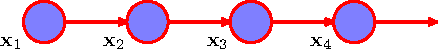
\includegraphics[]{figures/math/markov_chain}
  \caption{A graph model that represents the Markov chain.}
  \label{fig:mchain}
\end{figure}

\begin{figure}[p]
  \centering 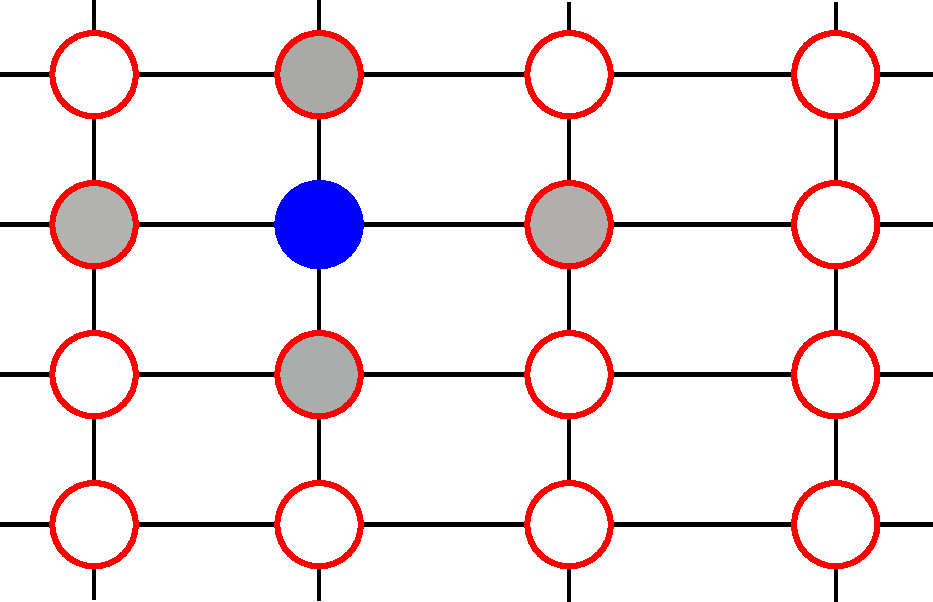
\includegraphics[width = 0.4\textwidth]{figures/math/mrf}
  \hspace{5pt} \includegraphics[width =
    0.4\textwidth]{figures/math/general_graph}
    \caption{Two graphical models represented by graphs. A graphical model
      representing a MRF can be either a regular grid or an general graph. For
      the regular grid, The node in blue color is conditional independent of
      the white node given it's adjacent neighbors, colored gray. For the
      general graph example, the two nodes in blue color are conditional
      independent given the remaining nodes. }
  \label{fig:mrf}
\end{figure}

\begin{figure}[p]
  \centering \includegraphics[width=0.5\textwidth]{figures/math/imagechain}
  \caption{A simulation of MRF. When a new candidate $w$ is accepted to replace
    current $x_s$, we get a new set of variables $X^{m+1}$ that differs from the
    current variable $X$ at only $s$. The set of variable $X^m$ and $W^{m+1}$
    is a sample of a Markov chain, since $X^{m+1}$ depends only on the previous
    $X^m$. Upon convergence, $X$ will be a sample from the target distribution
    $P(X)$. }
  \label{fig:imagechain}
\end{figure}

\begin{figure}[p]
  \centering
  \begin{subfigure}[b]{0.3\textwidth}
    \centering
    
\includegraphics[width=\textwidth]{figures/math/ising_sim/b08_1000}
    \caption{$\beta = 0.8$}
    \label{fig:beta0.8}
    \end{subfigure}
~
  \begin{subfigure}[b]{0.3\textwidth}
    \centering
    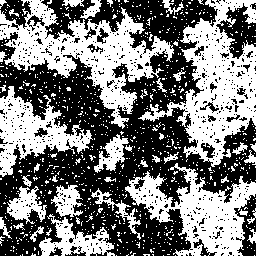
\includegraphics[width=\textwidth]{figures/math/ising_sim/b088_500}
    \caption{$\beta = 0.88$}
    \label{fig:beta0.88}
    \end{subfigure}
~
  \begin{subfigure}[b]{0.3\textwidth}
    \centering
    
\includegraphics[width=\textwidth]{figures/math/ising_sim/b10_1000}
    \caption{$\beta = 1.0$}
    \label{fig:beta1.0}
    \end{subfigure}

  \begin{subfigure}[b]{0.3\textwidth}
    \centering
    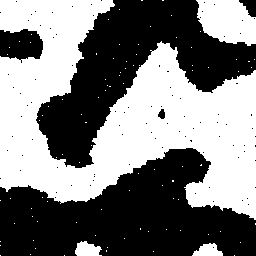
\includegraphics[width=\textwidth]{figures/math/ising_sim/b15_800}
    \caption{$\beta = 1.5$}
    \label{fig:beta1.5}
    \end{subfigure}
~
  \begin{subfigure}[b]{0.3\textwidth}
    \centering
    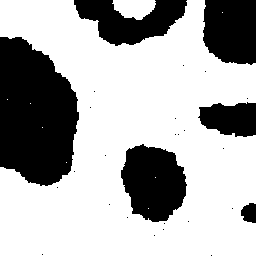
\includegraphics[width=\textwidth]{figures/math/ising_sim/b20_1000}
    \caption{$\beta = 2.0$}
    \label{fig:beta2.0}
    \end{subfigure}
~
  \begin{subfigure}[b]{0.3\textwidth}
    \centering
    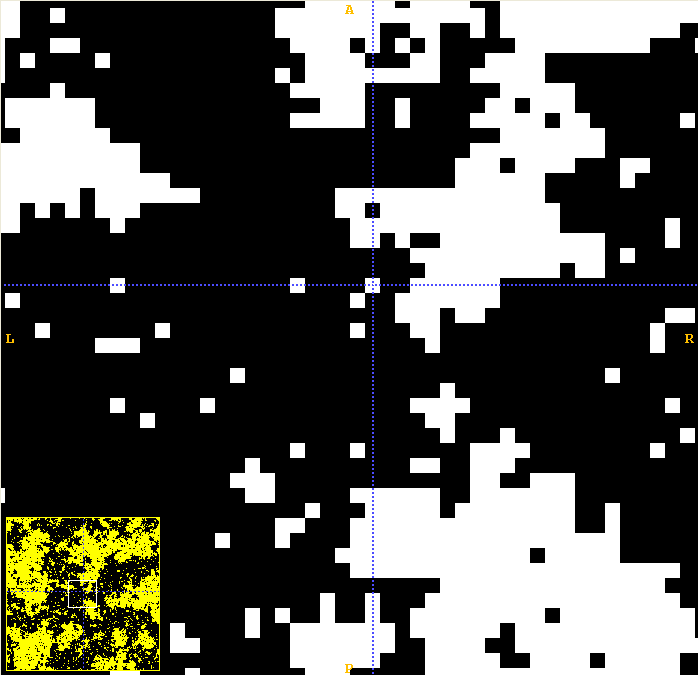
\includegraphics[width=\textwidth]{figures/math/ising_sim/b088_details}
    \caption{$\beta = 0.88$ zoomed in}
    \label{fig:beta0.88details}
    \end{subfigure}
  \caption{Simulating Ising model with various values of $\beta$. For each
    simulation, the image is initialized with random states, and then scanned
    1000 times. Notice when $\beta$ is small, the image is less spatially
    coherent. When $\beta$ is large, the image has more spatial coherent
    regions. }
  \label{fig:isingsim}
\end{figure}

\begin{figure}[p]
  \centering
  \begin{subfigure}[b]{0.3\textwidth}
    \centering 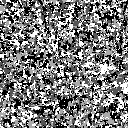
\includegraphics[width=\textwidth]{figures/math/potts_sim/b088}
    \caption{$\beta = 0.88$}
    \end{subfigure}
~
  \begin{subfigure}[b]{0.3\textwidth}
    \centering 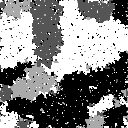
\includegraphics[width=\textwidth]{figures/math/potts_sim/b12}
    \caption{$\beta = 1.2$}
    \end{subfigure}
~
  \begin{subfigure}[b]{0.3\textwidth}
    \centering 
\includegraphics[width=\textwidth]{figures/math/potts_sim/b20}
    \caption{$\beta = 2.0$}
    \end{subfigure}
  \caption{Simulating Potts model of four states with various values of
    $\beta$. For all simulations, the image was initialized with random states,
    and then was scanned 1000 times. }
  \label{fig:pottssim}
\end{figure}

\begin{figure}[p]
  \centering 
  \begin{subfigure}[b]{\textwidth}
    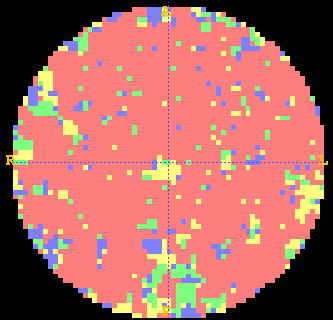
\includegraphics[width=0.3\textwidth]{figures/math/sw/gibbs1}
    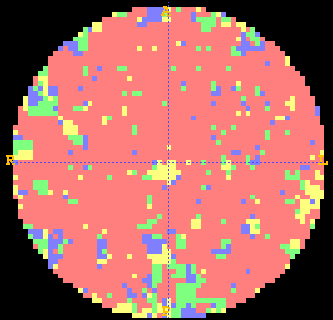
\includegraphics[width=0.3\textwidth]{figures/math/sw/gibbs2}
    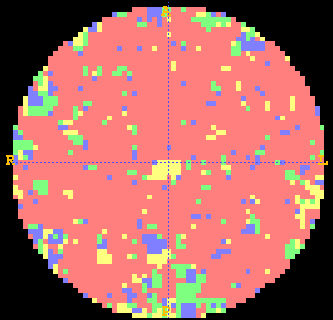
\includegraphics[width=0.3\textwidth]{figures/math/sw/gibbs3}
    \caption{Gibbs samples}
  \end{subfigure}
  ~
  \begin{subfigure}[b]{\textwidth}
    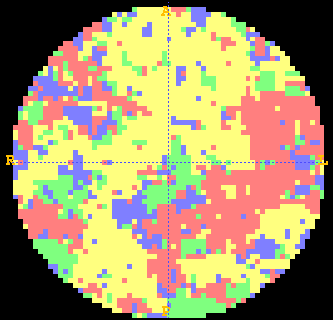
\includegraphics[width=0.3\textwidth]{figures/math/sw/sw1}
    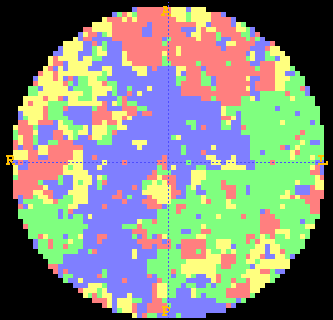
\includegraphics[width=0.3\textwidth]{figures/math/sw/sw2}
    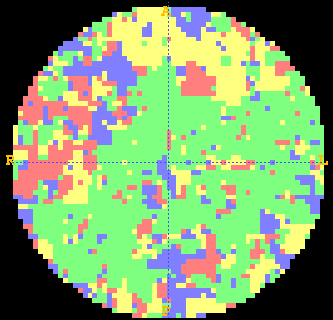
\includegraphics[width=0.3\textwidth]{figures/math/sw/sw3}
    \caption{SW samples}
    \end{subfigure}
    \caption{Consecutive samples of Potts model with $\beta = 1.1$ using SW
      and Gibbs sampling.  Both samplers initialize the sample image with
      all-zero values, have 100 burn-in sampling and then save three
      consecutive samples. Note for the SW samples, multiple voxel labels have
      been changed between the consecutive sample images. Such multiple
      updates speed up convergence. For Gibbs, the three sample images are
      similar due to the strong interactions (relatively large $\beta$)
      between the neighboring nodes. }
  \label{fig:mathsw}
\end{figure}

\begin{figure}[p]
  \centering \includegraphics[width = 0.5\textwidth]{figures/math/hmm}
  \caption{A graphical representation of the hidden Markov model(HMM). $X$ is
    defined on a regular lattice graph  and is given a MRF prior to represent
    our knowledge of the smoothness or piecewise constant. $Y$ is the observed
    data that is generated from the likelihood function given the hidden $X$.}
  \label{fig:hmm}
\end{figure}

\begin{figure}[p]
  \centering 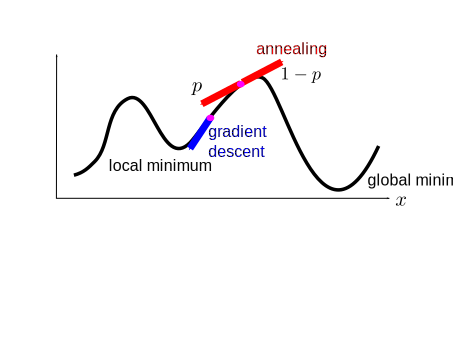
\includegraphics[width=0.6\textwidth]{figures/math/annealing}
  \caption{Simulated annealing samples one variable at a time. Unike
    coordinate descent that always moves in the gradient descent direction
    (blue color arrow), the SA algorithm updates the variable based on a certain
    probability, which depends on the difference of the function value of two
    configurations (red arrow).}
  \label{fig:annealing}
\end{figure}

\begin{figure}[p]
  \centering 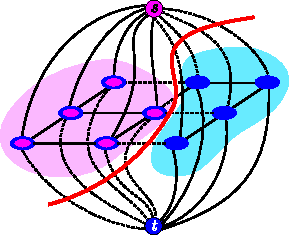
\includegraphics[width=0.5\textwidth]{figures/math/graphcuts}
  \caption{Graph cut segmentation. Each voxel is defined as a node on a
    graph. Neighboring voxels have edges between them with weights given by
    MRF. A source node $s$ and a sink node $t$ are added. All nodes have links to
    both sources and sink nodes with weights depend on the likelihood function
    (data term). Graph cut algorithms find a cut, i.e., a set of edges whose
    overall weights are minimized. In the figure, edges with solid lines are
    kept, and edges with dashed lines are removed after the cut. Red think links
    are the cut. Node is assigned to source or sink label if they are connected
    to either of them. }
  \label{fig:graphcuts}
\end{figure}

\begin{figure}[p]
  \centering 
  \begin{subfigure}[b]{0.3\textwidth}
  
\includegraphics[width=1\textwidth]{figures/math/gc/obs}
  \caption{Observed noise image}
  \end{subfigure}
~
  \begin{subfigure}[b]{0.3\textwidth}
  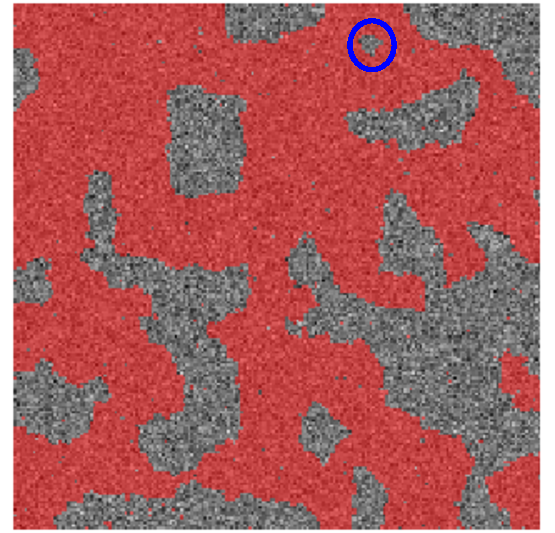
\includegraphics[width=1\textwidth]{figures/math/gc/truth_marked}
  \caption{Ground truth label map}
  \end{subfigure}
~
  \begin{subfigure}[b]{0.3\textwidth}
    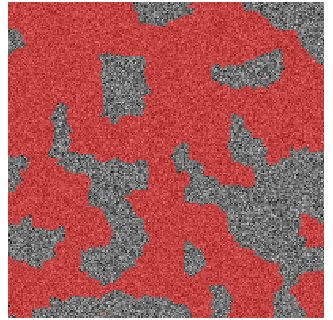
\includegraphics[width=1\textwidth]{figures/math/gc/rec}
    \caption{Recovered label map}
  \end{subfigure}


  \begin{subfigure}[b]{1\textwidth}
    \centering
    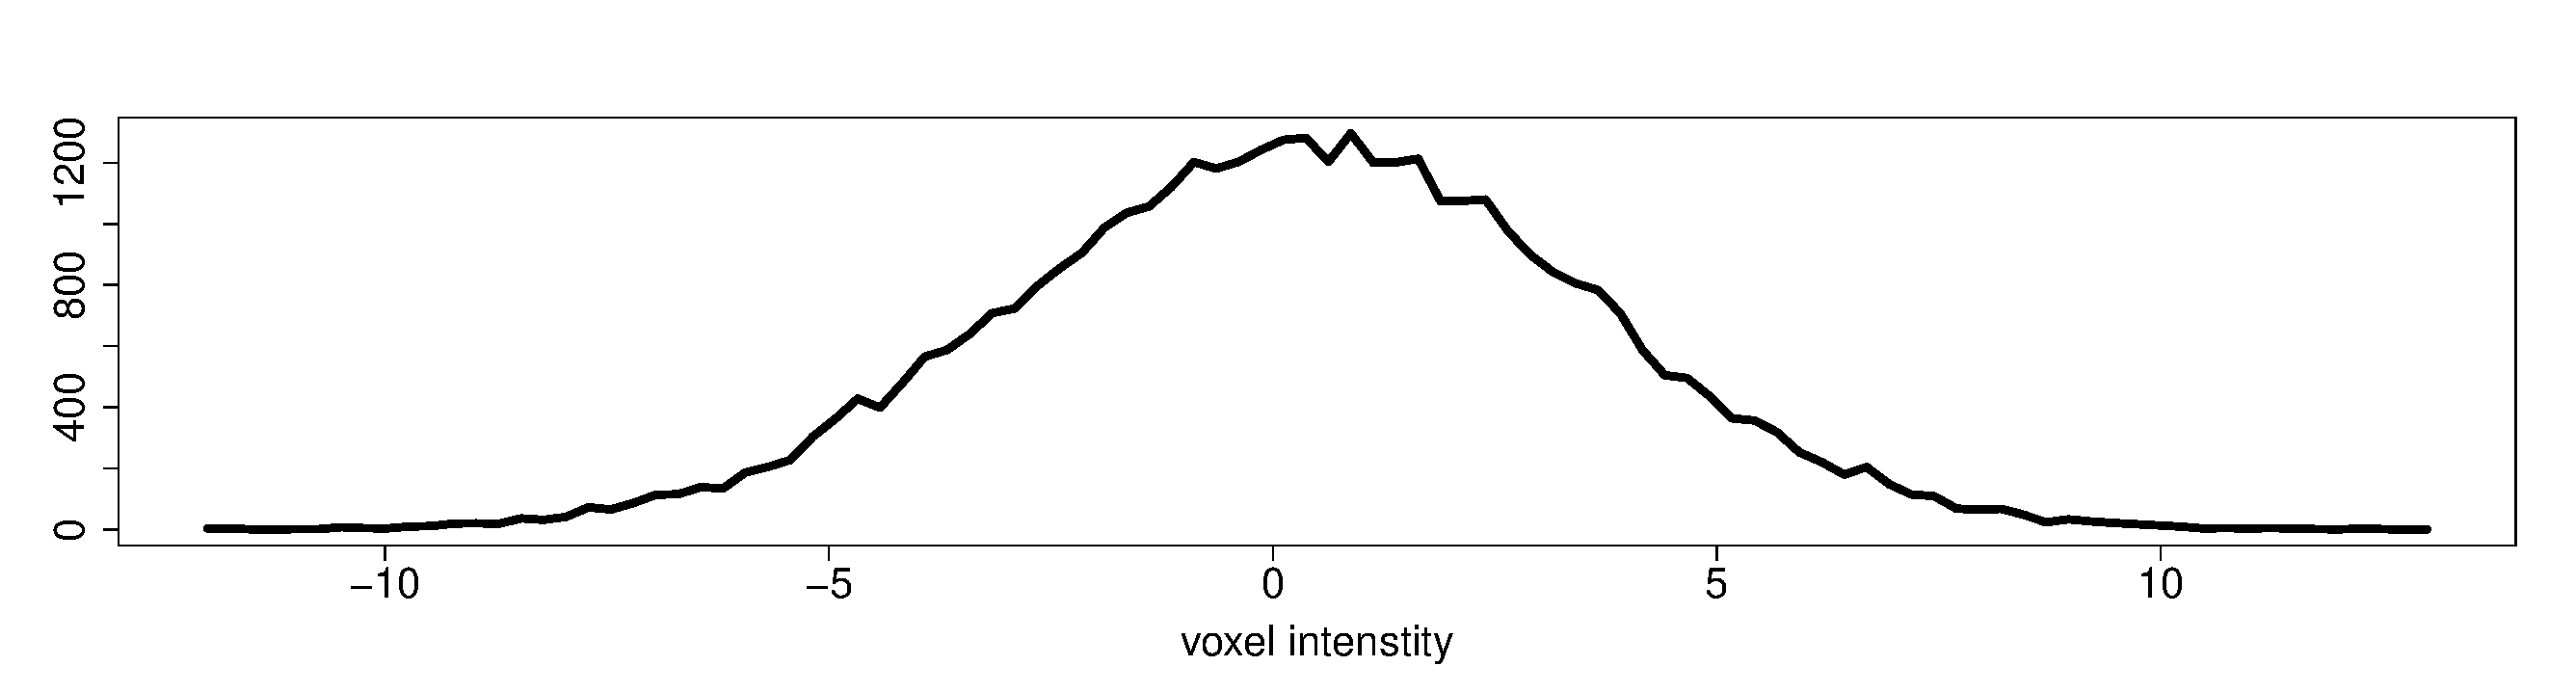
\includegraphics[width=0.8\textwidth]{figures/math/gc/hist}
    \caption{Histogram}
  \end{subfigure}

  \caption{Recovering noise image by graph cut. Top row from left to right:
    a) observed noised image, b) ground truth label map, c) recovered label
    map. Bottom d) histogram of the observed image intensity. Note the region in
    blue circle of the true map is misclassified. }
  \label{fig:gcexample}
\end{figure}

\begin{figure}[p]
  \centering 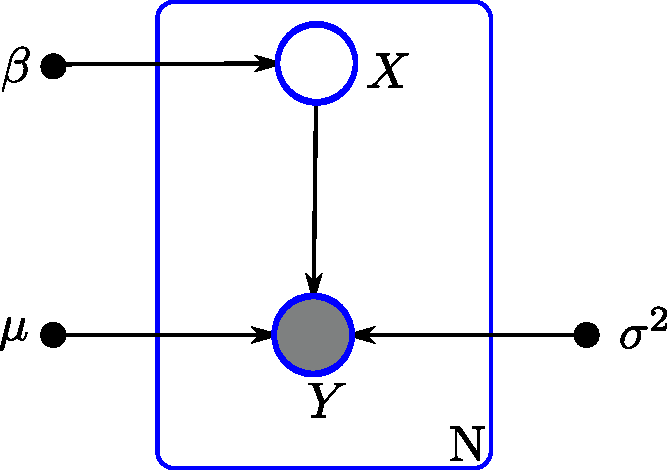
\includegraphics[width = 0.3\textwidth]{figures/math/paraest}
  \caption{A hidden Markov model with $X$ in MRF, and each $y_s$ is independent
    Gaussian given $x_s$. The parameters are black dots, the hidden variables
    are circles, and the observed data are grayed circles. The MRF structure on
    $X$ is not shown in this diagram. Instead a box is on $X$ and $Y$ to
    represent that there are $N$ such nodes. }
  \label{fig:paraest}
\end{figure}

\begin{figure}[p]
  \centering 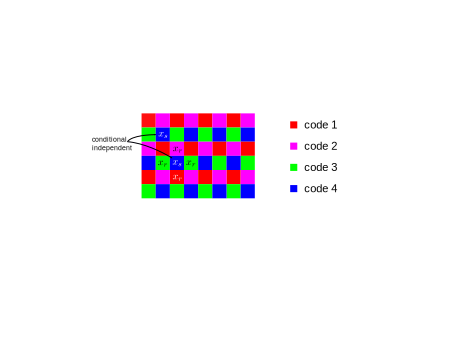
\includegraphics[width = 0.6\textwidth]{figures/math/coding}
  \caption{Coding scheme for parameter estimation. For four-neighbors system of two-dimensional
    image, the voxels are separated into four groups. The voxels in the same group
    are conditionally independent given other groups.}
  \label{fig:coding}
\end{figure}

\begin{figure}[p]
  \centering 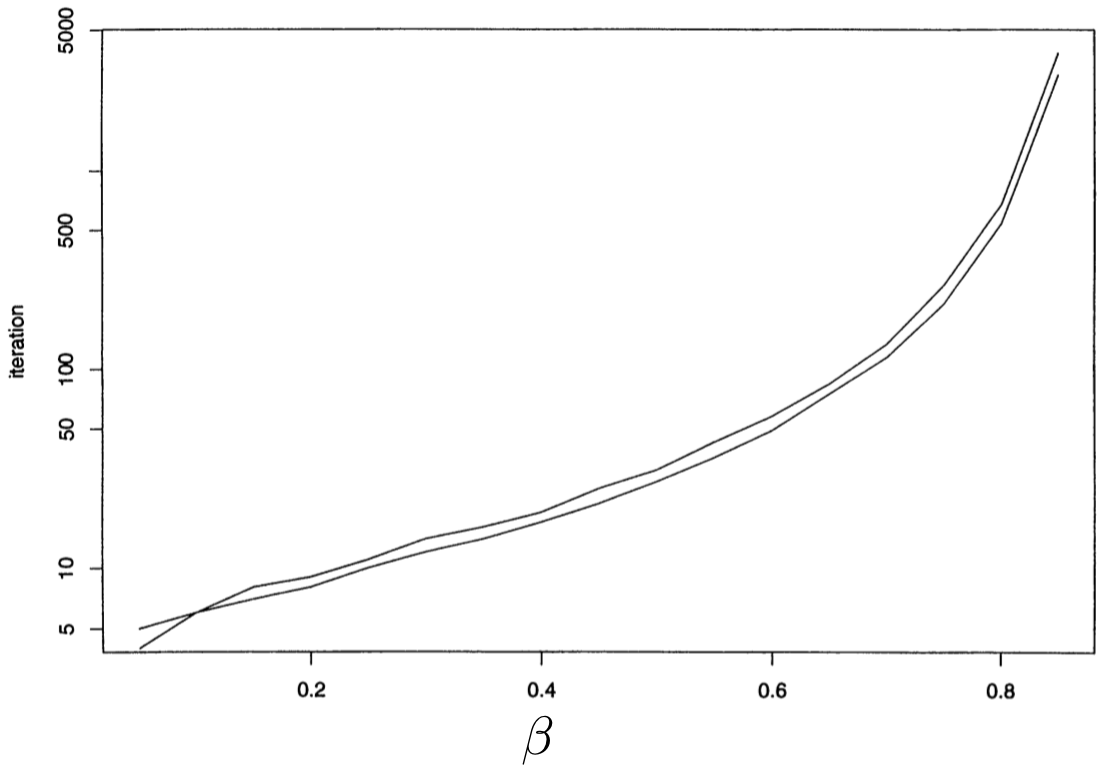
\includegraphics[width=0.7\textwidth]{figures/discussion/ising}
  \caption{Percentile of coupling iterations for Ising model of size $64\times
    64$. Top curve shows the 99\% and bottom shows the 95\% percentile from the
    distribution of the iterations needed for coupling, as a function of $\beta$
    parameter.  The percentiles are estimated using 1000 repetitions of Gibbs
    sampling initialized with all-white and all-black value. (adapted from
    Johnson~\cite{johnson1996studying}. }
\label{fig:ising}
\end{figure}

%%% Local Variables: 
%%% TeX-master: "MyThesis"
%%% End: 

\chapter{Full Pairwise Connectivity With Spatial Coherence}
\label{chap:method1}

% the functional activity has the multiple comparision problem. 
In this chapter, we present a new method for spatial regularization of
functional connectivity maps based on MRF priors. The high level of noise in
fMRI leads to errors in functional connectivity detection algorithms. A common
approach to mitigate the effects of noise is to apply spatial Gaussian
smoothing, which can lead to blurring of regions beyond their actual boundaries
and the loss of small connectivity regions. Recent work has suggested MRF as an
alternative spatial regularization in the detection of fMRI activation in
task-based paradigms. We propose to apply MRF priors to the computation of
functional connectivity in resting-state fMRI. Our Markov priors are in the
space of pairwise voxel connections, rather than in the original image space,
resulting in a MRF whose dimension is twice that of the original image. The high
dimensionality of the MRF estimation problem leads to computational
challenges. We present an efficient, highly parallelized algorithm on the
graphics processing unit (GPU). We validate our approach on a synthetically
generated example as well as real data from a resting state fMRI study.

\section{Motivation}
To show the noise level and the impact of spatial smoothing on the functional
connectivity estimation, we take a seed voxel at the MNI coordinate (42, 16, 25)
and compute the correlation between this seed region and every other voxel's
BOLD signal in the same volume of the spatially smoothed rs-fMRI volume, and
show the correlation map at Figure \ref{fig:conexample}. The seed signal is
computed by averaging the BOLD signal of voxels within 5 mm distance from the
seed voxel. Following  standard seed-based functional connectivity methods,
we average the BOLD signal of the voxels within r = 5 mm from the seed voxel,
and use the averaged signal as a surrogate of the BOLD signal at this
coordinate. We then compute the sample correlation between this average signal
and every other voxel's BOLD signal in the full volume. For display purposes, we
only show the correlation map of one slice where the seed region is
located. Figure \ref{fig:fmrislice} shows the first time point of the original
BOLD signal. As expected, it is impossible to see any meaningful patterns from
this image, since the functional connectivity is not represented by a voxel's
intensity at a single time point, but the average effect across all time
points. Figure \ref{fig:corrmap} shows the linear correlation map with the seed
regions, with the red dot giving the location of the seed region. We can see the
symmetric location of the seed region on the other hemisphere shows higher
intensity of correlation, suggesting these voxels are more positively correlated
with the seed. In Figure \ref{fig:corrmap_th}, we show the correlation map
thresholded at 0.3. Since the seed region belongs to the default model network
(DMN), an important component in the intrinsic functional system, we expect to
see other spatially remote regions in the same network have higher correlation
in \ref{fig:corrmap_th}, We observe one region on the same location of the
opposite hemisphere, and also one region at the prefrontal lobe remains after
thresholding. However, overall the spatial patterns are hard to identify, and there
are also some false-positive detections. One reason for the difficulty in
detecting the connectivities is the large amount of noise in the data, and the
spatial smoothing in the preprocessing step. We aim to address this problem in
this chapter.


In both task-based and rs-fMRI the impact of imaging noise can be reduced by
taking advantage of the spatial correlations between neighboring voxels in the
image. A common approach used for instance in statistical parametric mapping
(SPM)\cite{worsley_analysis_1995} is to apply a spatial Gaussian filter to
smooth the signal prior to statistical analysis. However, this can lead to
overly blurred results, where effects with small spatial extent can be lost and
detected regions may extend beyond their actual boundaries. An alternative
approach to spatial regularization that has been proposed for task activation
paradigms is to use a Markov random field (MRF) prior~\cite{ou_spatial_2005,
  descombes_spatio-temporal_1998, descombes_fmri_1998,
  woolrich_fully_2004,cosman_exact_2004}, which models the conditional
dependence of the signals in neighboring voxels.

In this chapter we propose to use MRF models in rs- fMRI to leverage spatial
correlations in functional connectivity maps. Unlike previous MRF-based
approaches, which use the neighborhood structure defined by the original image
voxel grid, the neighborhoods in functional connectivity must take into account
the possible relationships between spatially distant voxels. Therefore, we
define the neighborhood graph on the set of all voxel pairs. This results in a
Markov structure on a grid with twice the dimensions of the original image data,
i.e., the pairwise connectivities for three-dimensional images results in a
six-dimensional MRF. The neighborhood structure is defined so that two voxels
are more likely to be connected if they are connected to each other's spatial
neighbors.

We combine the Markov prior on functional connectivity maps with a likelihood
model of the time series correlations in a posterior estimation problem.
Furthermore, we  solve for the unknown parameters of the MRF and likelihood
using the EM algorithm that we discussed in Section \ref{chap:em}. In the
estimation step the posterior random field is sampled using Gibbs sampling and
estimated using mean field theory, also known as variational inference.

In the next section we describe our MRF model of functional connectivity maps.
In Section~\ref{sec:methods} we give the details of the algorithm to estimate
the functional connectivity probabilities, including implementation details for
the GPU solver. Finally, in Section~\ref{sec:results} we demonstrate the
advantages of our approach on a synthetically generated data set as well as on
real rs-fMRI data.

\section{Methods}
\label{sec:methods}
Our framework for functional connectivity is a Bayesian approach in which we
estimate the posterior distribution of the connectivity between voxels,
conditioned on the fMRI data. Let $X = \{x_{ij}\}$ denote the functional
connectivity map, i.e., a map denoting whether each pair of voxels $i,j$ is
connected, and let $Y$ denote the original fMRI data, or some measurement
derived from the fMRI. In this work we take $Y$ to be the map of correlations
between pairs voxel time series. The posterior distribution is then
proportionally given by
\begin{equation}
\label{eq:posterior}
P(X \, | \, Y) \prop P(X) \cdot P(Y \, | \, X).
\end{equation}
In this work we model $P(X)$, the prior on the connectivity map, using a
MRF, and the likelihood $P(Y \, | \, X)$ using Gaussian models of the
Fisher transformed correlation values. We now give details for both of these
pieces of the model.


\subsection{Markov prior}
Conventional image analysis applications of MRFs~\cite{li_markov_2009} define
the set of sites of the random field as the image voxels, with the neighborhood
structure given by a regular lattice. Because we are studying the pairwise
connectivity between voxels, we need to define a MRF in the higher-dimensional
space of voxel location pairs. Thus, if $\Omega \subset \mathbb{Z}^d$ is a
$d$-dimensional image domain, then the sites for our connectivity MRF form the
set $\mathcal{S} = \Omega \times \Omega$. Let $i, j \in \Omega$ be voxel
locations, and let $\mathcal{N}_i, \mathcal{N}_j$ denote the set of neighbors of
voxel $i$ and $j$, respectively, in the original image lattice. Then the set of
neighbors for the site $(i, j) \in \mathcal{S}$ is given by $\mathcal{N}_{ij} =
(\{i\} \times \mathcal{N}_j) \cup (\mathcal{N}_i \times \{j\})$. In other words,
two sites are neighbors if they share one coordinate and their other coordinates
are neighbors in the original image lattice. This neighborhood structure will
give us the property in the MRF that two voxels $i, j$ in the image are more
likely to be connected if $i$ is connected to $j$'s neighbors or
vice-versa. Equipped with this graph structure, $\mathcal{S}$ is a regular
$2d$-dimensional lattice. With the node set $\cX$ and neighboring system $\cN$,
we define a graph $\cG$ that we call the {\em connectivity graph}. Figure
\ref{fig:6dmrf} gives an illustration of how this connectivity graph is defined.

We next define a multivariate random variable $X = \{ x_{ij} \}$ on the set
$\mathcal{S}$, where each $x_{ij}$ is a binary random variable that
denotes the connectivity ($x_{ij} = 1$) or lack of connectivity ($x_{ij} = -1$)
between voxel $i$ and $j$. If $A \subset \mathcal{S}$, let $X_A$ denote the
set of all $x_{ij}$ with $(i,j) \in A$, and let $X_{-ij}$ denote the
collection of all variables in $X$ excluding $x_{ij}$. For $X$ to be a
MRF it must satisfy
\begin{equation*}
  P( x_{ij} \, | \, X_{-ij}) = p(x_{ij} \, | \, x_{\mathcal{N}_{ij}}).
\end{equation*}
According to the Hammersley and Clifford theorem~\cite{besag_spatial_1974}, $X$
is a Markov random field if and only if it is also a Gibbs distribution, defined
as
\begin{equation}
  P(X) = \frac{1}{Z}\exp\left(-U(X)\right), 
\end{equation}
where $U$ is the energy function $U(X) = \sum_{c \in \mathcal{C}}
V_c$, with potentials $V_c$ defined for each clique $c$ in the clique
set $\mathcal{C}$. The partition function $Z = \sum_{X} \exp(-U(X))$
is a normalizing constant, where the summation is over all possible
configurations of $X$. We use a particular form of MRF---the
Ising model---a commonly used model for MRFs with binary states. In
this model the energy function is given by
\begin{equation}
U(X) = - \beta \sum_{( ij, mn )} x_{ij} x_{mn},
 \label{eq:A1}
\end{equation}
where the summation is over all edges $( ij, mn )$ on the graph $\cG$, i.e., all
adjacent voxel pairs $(i,j), (m,n)$ in the connectivity graph. When $\beta > 0$,
this definition favors similarity of neighbors. An alternative definition is to
make the MRF prior also contain the data term, such as the strength of the
connection between neighboring nodes also depends on the data. Where the
observed correlation value of two nodes are different, the strength of the MRF
prior will be decreased. This is the conditional random field we have discussed
in Section \ref{sec:crf}.
\subsection{Likelihood model}
We now define the likelihood model, $P(Y \, | \, X)$, which connects the
observed data $Y$ to our MRF. Because we are interested in the functional
connectivity between pairs of voxels, we compute the correlation between the
time courses of each pair of voxels, and get a correlation matrix $Y =
\{y_{ij}\}$. Just as in the case of the random field $X$, the correlation matrix
$Y$ is also defined on the $2d$-dimensional lattice $\mathcal{S}$. Linear
correlation is not the only choice for $Y$. We can use any statistic, as long as
it indicates the affinity between two voxel time series. Another possibility
could be frequency domain measures, such as the
coherence~\cite{mller_multivariate_2001}, although the definition of likelihood
function is not straightforward for such similarity measurement. On the other
hand, simple linear correlation has the advantage that after the Fisher
transformation, the correlation statistics have a well defined distribution. If
the original variables $y_i$ and $y_j$'s intensities across all time points are
Gaussian, then the sample correlation estimated from the intensities are also
Gaussian after Fisher transformation. Therefore, the conditional distribution of
$P(y_{ij} | x_{ij})$ is a well-defined Gaussian distribution.

Before defining the full data likelihood, we start with a definition of the {\em
  emission function} at a single site $s_{ij} \in \mathcal{S}$. This is defined
as the conditional likelihood, $P(y_{ij} \, | \, x_{ij})$, and is interpreted as
the probability of the observed correlation, given the state of the connectivity
between voxels $i$ and $j$. We model the emission function as a Gaussian
distribution with unknown mean and variance on the Fisher transformed
correlation $y_{ij}$, that is,
\begin{equation}
\label{eq:emission}
P(y_{ij} \,|\, x_{ij} = k) = \frac{1}{\sqrt{2\pi} \sigma_k} \exp \left( -\frac{(F(y_{ij}) -  \mu_k)^2}{2\sigma_k^2}\right),
\end{equation}
where $F$ denotes the Fisher transform. Notice that each correlation $y_{ij}$ on
site $s_{ij}$ only depends on the latent variable $x_{ij}$ on the same site, and
does not depend on neighbors of $x_{ij}$. Alternative definitions exist. For
example, the observed correlation data $y_{ij}$ can also depend on the
neighbors of $x_{ij}$, similar to the work of Geman et
al.~\cite{geman1984stochastic}. This is equivalent to adding more edges on the
graphical model, and therefore the posterior inference will be more
complicated. In this work, we use a simple model that has a one-to-one
correspondence between $x_{ij}$ and $y_{ij}$. Given the above setting, the full
likelihood is given by
\begin{equation}
\label{eq:likelihood}
P(Y \, | \, X) = \prod_{s_{ij}\in\mathcal{S}} P(y_{ij} \, | \, x_{ij}).
\end{equation}

\section{Estimation via expectation maximization}
\label{sec:algorithm}
Having defined the data likelihood and MRF prior in the previous section, we are
now ready to describe the maximization of the posterior given
by~\eqref{eq:posterior}. For this we need to determine the model parameters,
$\beta$ in \eqref{eq:A1} and $(\mu_k, \sigma_k^2)$ in
\eqref{eq:emission}. Rather than arbitrarily setting these parameters, we
estimate them using the EM algorithm. Exact
computation of the full posterior~\eqref{eq:posterior} is intractable, due to
the combinatorial number of terms in the partition function $Z$. Therefore, we
instead maximize the approximate posterior given by the pseudo-likelihood
function~\cite{li_markov_2009,besag_spatial_1974},
\begin{equation}
PL(X, Y) = \prod_{ij}^{}P (x_{ij}|x_{\mathcal{N}_{ij}}) P(y_{ij}|x_{ij}). \label{eq:2}
\end{equation}

In the E-step, the parameters are held fixed and we compute the posterior
probability for each $x_{ij}$, and sample $x_{ij}$ from the posterior
distribution using Gibbs sampling. We then compute the expected value of each
connectivity node by mean field theory. After we compute the posterior of
current point $x_{ij}$, we update $x_{ij}$ with its expected value $\langle
x_{ij} \rangle$. The equivalence of posterior probability and the expectation of
binary random variable is discussed in Section \ref{chap:mathvar}.

In the M-step, the complete data $\{\langle X\rangle, Y\}$ are available, and the
parameters can be estimated by maximizing the joint pseudo-likelihood given
by~\eqref{eq:2} using Newton's method. After several iterations of this EM
algorithm, we get parameters as our MAP estimates. During parameter estimation,
the joint likelihood can be factorized into two separate terms of the prior and
the conditional likelihood, and the parameter $\beta$ can be estimated by
maximizing the MRF prior (equivalently the pseudo-likelihood) by Newton's
method. The estimation of $\mu$ and $\sigma^2$ can be done in closed from just
like the standard Gaussian mixture model, as shown in Section \ref{sec:parest}.

\subsection{GPU implementation}
 The whole algorithm involves updating a high dimensional connectivity matrix
 $X$ iteratively, and hence it has high computation cost. We designed a parallel
 Markov random field updating strategy on a graphics processing unit (GPU). The
 algorithm takes only a few minutes compared with more than 1 hour on the CPU
 counterpart.


To fit the algorithm into GPU's architecture, we use some custom
strategies. First, because GPU only support three-dimensional array, we need to
reshape $X$ and $Y$ defined originally on a higher dimensional graph by linear
indexing their original subscripts. This is especially difficult for brain fMRI
data because the gray matter voxels reside in an irregular three-dimensional lattice. Specific
data structures are used for mapping between original voxel subscripts and their
linear index $i$ and $j$. Second, to update each site of the MRF in parallel, we
have to make sure a site is not updated simultaneously with its neighbors,
otherwise the field tends to be stuck in a checkerboard-like local maximum, as
indicated by Figure \ref{fig:checkerboard}.  Our strategy is to divide all the
sites of the field into several subgroups, such that a site is not in the same
subgroup with its neighbors.  We then can update the subgroup sequentially,
while the data in subgroups are updated simultaneously. The whole procedure is
summarized in Algorithm \ref{alg:1}.


\begin{algorithm}[p]
  \caption{MAP estimation by EM}
  \label{alg:1}
  \begin{algorithmic}
    \REQUIRE Sample correlation matrix $\mat Y$.
    \STATE Init posterior matrix by maximizing conditional likelihood
    $P(y_{ij}|x_{ij})$.  
    \WHILE{$\Delta \{\beta, \mu, \sigma^2 \} >
      \varepsilon$ } 
    \STATE \textbf{E step: }

    (a) Based on the current
    parameters, compute the posterior by \eqref{eq:2}.

    (b) Repeatedly Do Gibbs Sampling until the field  stabilizes.

    (c) Based on current value of $x_{ij}$, iteratively compute the mean
    field for all nodes in $\mathcal{S}$ until the field is stable.

    \STATE \textbf{M step: } 

    (d) With complete data $\{\mat X, \mat
    Y\}$, estimate $\beta$ , $\mu$ and $\sigma^2$ by maximizing
    \eqref{eq:2}.
    \ENDWHILE
    \RETURN posterior matrix $\mat X$.
  \end{algorithmic}
\end{algorithm}

It is noted this updating scheme is closely related to the coding method of
parameter estimation of MRF that we discussed in Section \ref{sec:parest}. Both
approaches split the variables into multiple subgroups. They differ in that
for coding methods, the separation is used to get independent variables within
the subgroup, while here the voxels in subgroups are independent so we can
update them in parallel.


\section{Results}
\label{sec:results}
In this section, we give the experimental results for both  simulated data and
real fMRI data. We compare the results of various methods on simulated data
with the ground truth to show the proposed method's performance. In the real
data experiment, we compare the results with the functional connectivity map of
other literatures.


\subsection{Synthetic data} 
\label{sec:m1syn}
We first construct a synthetic data set consisting of a $100\times 1$
one-dimensional image, with each pixel a 300-point time course signal. The
one-dimensional image will guarantee the connectivity map be in
two-dimensional space and can be visualized easily. The time course was
constructed with a baseline DC signal of 800, plus additive Gaussian noise of
zero mean and variance 50. We then added a sine wave signal of frequency 0.2
and amplitude 20 to two distant regions of the image. The goal is to detect
the connectivity between these two distant regions. The true connectivity
value will be one between those pixels containing the sine wave signal,
otherwise it is defined as $-1$ for lack of connectivity between signal and
noise, and between noise time series. The true connectivity map is shown in
Figure~\ref{fig:6dconn1}.

To compare our MRF model with conventional Gaussian blurring of the correlation
map, we applied both approaches to the synthetic data (Figure
~\ref{fig:6dconn}). On the correlation map in the top row, we see smoothing does
remove noise and results in a correlation map that looks more like the true
connectivity map. However, it also creates several errors, most noticeably false
positives around the diagonal (Figure~\ref{fig:6dconn5}). This is because
without prior knowledge of the scale of the patterns we are interested in, the
choice of smoothing kernel size is arbitrary. Therefore, a large kernel size
will enforce the signals of many voxels to look similar, and the following correlation
map will have more false-positive detections. Figure~\ref{fig:6dconn6} shows the
proposed MRF method better detects the true connectivity regions while removing
most false positives.
 

\subsection{Resting-state fMRI} 
Next we tested our method on real data from healthy control subjects in a
resting-state fMRI study. BOLD EPI images (TR= 2.0 s, TE = 28 ms, GRAPPA
acceleration factor = 2, 40 slices at 3 mm slice thickness, 64 x 64 matrix, 240
volumes) were acquired on a Siemens 3 Tesla Trio scanner with 12-channel head
coil during the resting state, eyes open. The data was motion corrected by SPM
software and registered to a T2 structural image. We used a gray matter mask
from an SPM tissue segmentation so that only gray matter voxels are counted in
the connectivity analysis. We do \emph{not} spatially smooth the data, in order
to see the benefit of replacing spatial smoothing with our MRF method. Before
computing the correlations, the time series at all voxels are linearly detrended
by least squares regression.

Figure \ref{fig:invivo1} compares the real data results using no spatial
regularization, Gaussian smoothing, and the proposed MRF model. Though the
posterior connectivity of the MRF is computed between every pair of voxels
within a slice, for visualization purposes, only the posterior of the
connectivity between one voxel and the slice is shown. We chose to visualize
the connectivity to a voxel in the posterior cingulate cortex (PCC) because
this is known to be involved in the default mode
network~\cite{raichle2001default}, with connections to the medial prefrontal
cortex (MPFC). The results show that Gaussian smoothing is able to remove
noise, but is unable to find a clear connection between the PCC and the
MPFC. Our proposed MRF model (\ref{fig:invivo13} and \ref{fig:invivo16}) is
able to remove spurious connections, and also clearly shows a connection to
the MPFC.

To show the strongest connections found by each method, Figure
\ref{fig:invivo2} shows the thresholded connectivity maps overlaid on T2
structural image. Images in the first two columns are thresholded such that
the top $5\%$ voxel correlations are shown. For the MRF in \ref{fig:invivo23}
and \ref{fig:invivo26}, the MAP estimate is shown.


\section{Discussion}
Functional connectivity is a key step of understanding the human brain's
functional networks, since it contains all the information of how each
functional region interacts with other regions. There are multiple ways of
modeling functional systems. One is defining some regions of interest (ROI) as
the nodes on the graph, and estimate the connectivities among these ROIs. The
ROI definition has no standard to follow. One can either define them according
to the anatomical structure, or by a parcellation on the functional data. The
other way of representing functional networks is to cluster the full brain
volume (indeed the gray matter voxels) into small regions. Regions in the same
cluster are highly connected even if they are spatially remote. Our method
outputs a posterior matrix that includes all the connectivity information between
each pair of voxels. One potential usage of the full connectivity matrix is 
exploring the connectivity given a single seed coordinate. That is, given the
seed, one can explore the posterior connectivity between the seed voxel and the
full brain volume in real time. Such full connectivity will be dynamically
shown with the changing seed's location. Such a dynamic, and potentially
user-interactive functional connectivity exploratory concept has been partly
realized by Yeo et al.~\cite{yeo2011organization}, though they did not use MRF
to model the spatial constraints of the connectivity variables. Instead, Yeo
et al. use
a large group of subjects and obtained a highly consistent population functoinal
connectivity network. The network can be visualized given a seed region and also
the change of the network patterns when the seed changes.

On the optimization side, the MCEM algorithm, and the wider class of sampling
methods are potentially good candidates for the application of GPU. Although
theoretically the computation on GPU needs independence between the data
points, the order of voxels being sampled have no effect on the quality of the
samples once the sampling reaches stationary distribution. Therefore, even at
each scan, the order, or the schedule of the data points change in an
undetermined way within the GPU cores, we can still get samples in the target
distribution give enough burn-in time. Alternative optimization methods other
than MCEM exist, such as graph cut. However, in our experiments with graph
cuts, we found the local finer patterns are sometimes ignored by graph
cut. The estimated hidden variables are accordingly mostly blob-like patterns
with small boundary-area ratio. So graph cut optimization is more suitable for
the recognition of blob-like patterns. Such preference does not necessarily
reflect the true structure in our fMRI data. As a result, the estimation of
the parameters $\beta$ in \eqref{eq:A1} is also biased towards a larger value
than the true value, since the true $X$ is not as smooth as the estimated
one. Therefore, we choose to use MCEM in our EM procedure for unbiased
estimation of parameters.

One weakness of the pairwise connectivity estimation routine is lack of
visualization for all the functional networks as spatial maps. Only when the
input image is one-dimensional, such as the synthetic data example we used in
Section \ref{sec:m1syn}, can the connectivity map be visualized on a
two-dimensional plane. In general three-dimensional volume image as input, the
connectivity matrix is in a six-dimensional space and cannot be shown in a
straightforward way. Once the posterior connectivity matrix is computed, we
still need to give a seed region in order to map all the functional systems
that are connected to the seed. We will discuss methods of estimating multiple
functional networks and show them in a single volume image in the next
chapter.



\begin{figure}[p]
  \centering
  \begin{subfigure}[b]{0.3\textwidth}
    \centering
    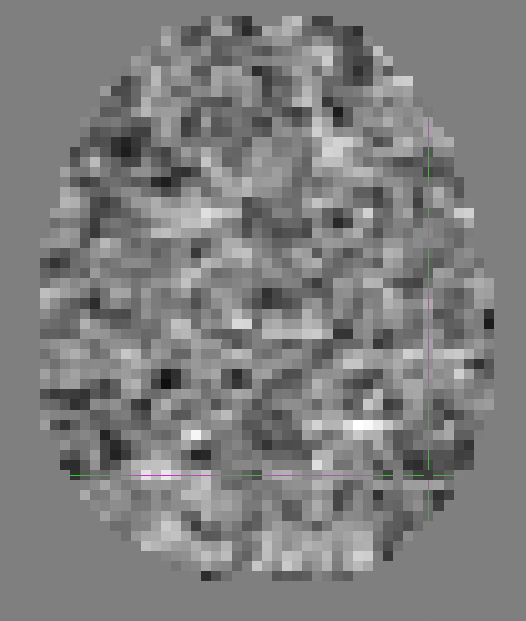
\includegraphics[height=\textwidth]{figures/method1/fmrislice}
    \caption{One slice of a resting-state fMRI dataset at $z = 25$. }
    \label{fig:fmrislice}
    \end{subfigure}
~
  \begin{subfigure}[b]{0.3\textwidth}
    \centering
    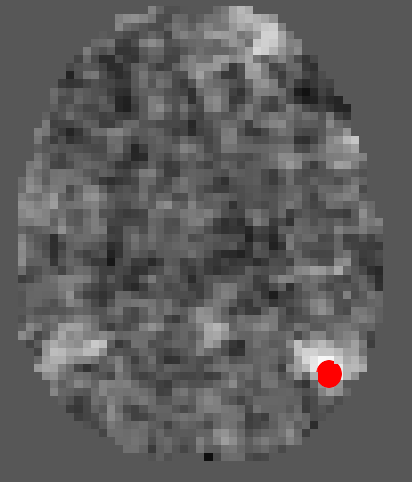
\includegraphics[height=\textwidth]{figures/method1/corrmap}
    % x = 42, y = 16, z = 25
    \caption{Correlation map between a seed and the current slice.}
    \label{fig:corrmap}
    \end{subfigure}
~
  \begin{subfigure}[b]{0.3\textwidth}
    \centering
    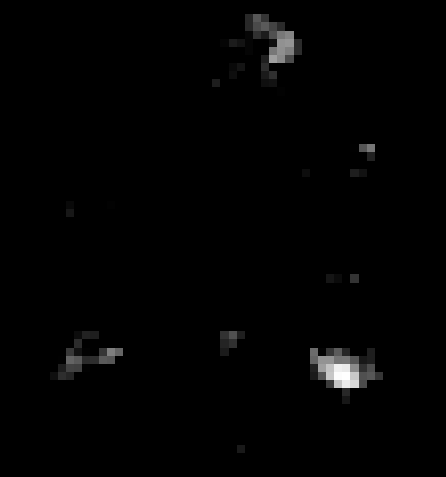
\includegraphics[height=\textwidth]{figures/method1/corrmap_th}
    \caption{The correlation map thresholded at 0.3.}
    \label{fig:corrmap_th}
    \end{subfigure}
  \caption{An example of correlation map with a seed in the default model
    network on the rs-fMRI data set.}
  \label{fig:conexample}
\end{figure}

\begin{figure}[p]
  \centering
  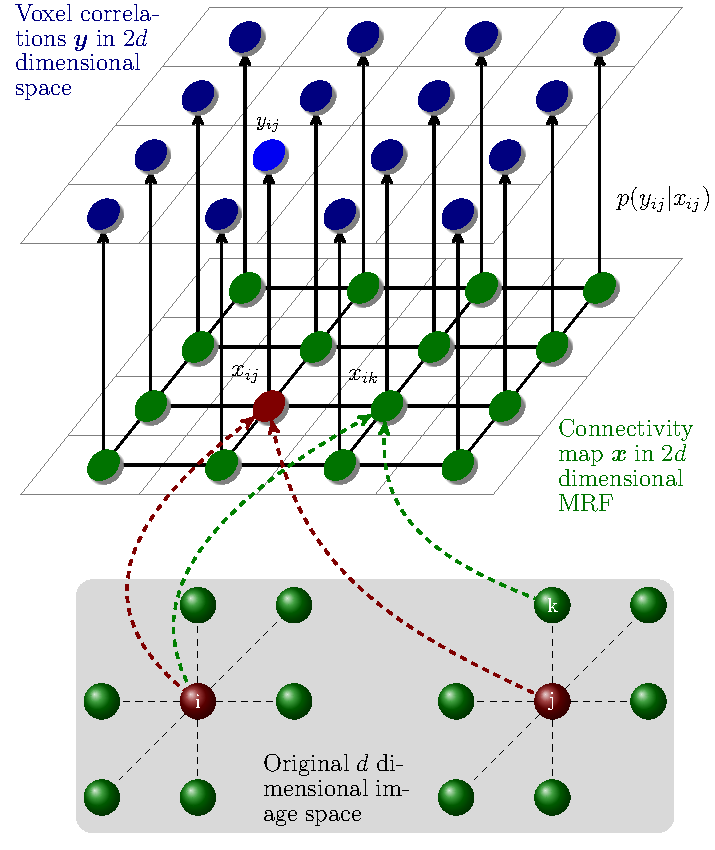
\includegraphics[width=0.5\textwidth]{figures/method1/6dmrf}
  \caption{MRF prior of the connectivity variables. Each node of the graph
    represents a pairwise connectivity variable between voxel $i$ and $j$. An
    edge is added between two nodes $x_{ij}$ and $x_{ik}$ if $k$ is the neighbor
    of voxel $j$. The graph where the MRF is defined is twice the dimensions
    of the original image domain, i.e., six dimensions. Given the hidden variable
    $X$, the observed sample correlation values are assumed to be generated
    from a Gaussian distribution with unknown parameter $\cN(y_{ij} | x_{ij}; \mu,
    \sigma^2)$. }
  \label{fig:6dmrf}
\end{figure}

\begin{figure}[p]
  \centering
  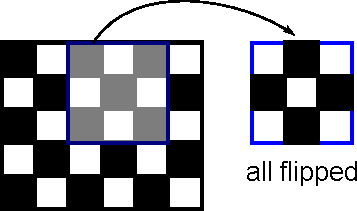
\includegraphics[width=0.5\textwidth]{figures/method1/checkerboard}
  \caption{Ideally the update of each voxel is independent of other voxels in
    order to be used on the GPU. In our Gibbs sampling, although the sampling of
    each voxel depends on its neighbors, the order of the voxels being updated
    does not matter. Upon convergence, the image will be a sample of the target
    Gibbs distribution. However, numerically, the sampling tends to be stuck in
    this local minimum of checkerboard image. At the current state, each voxel has a
    neighbor with a different state, and the sampling flips the color
    of all voxels in the next stage.}
  \label{fig:checkerboard}
\end{figure}

\begin{figure}[p] 
  \centering 
  \begin{subfigure}[t]{0.3\textwidth}
    \centering
    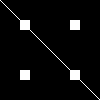
\includegraphics[width=\textwidth]{figures/method1/newtoy/trueConn}
    \caption{ground-truth connectivity}
    \label{fig:6dconn1}
    \end{subfigure}
~
  \begin{subfigure}[t]{0.3\textwidth}
    \centering
    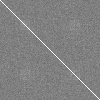
\includegraphics[width=\textwidth]{figures/method1/newtoy/corrNoSmooth}
    \caption{ correlation of original, noisy data.}
    \label{fig:6dconn2}
    \end{subfigure}
~
  \begin{subfigure}[t]{0.3\textwidth}
    \centering
    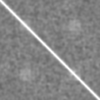
\includegraphics[width=\textwidth]{figures/method1/newtoy/SampleCorr}
    \caption{correlation of Gaussian-smoothed data.}
    \label{fig:6dconn3}
    \end{subfigure}

  \begin{subfigure}[t]{0.3\textwidth}
    \centering
    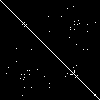
\includegraphics[width=\textwidth]{figures/method1/newtoy/threholdCorrRaw}
    \caption{connectivity based on noisy correlations.}
    \label{fig:6dconn4}
    \end{subfigure}
~
  \begin{subfigure}[t]{0.3\textwidth}
    \centering
    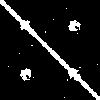
\includegraphics[width=\textwidth]{figures/method1/newtoy/threholdCorrSmoothed}
    \caption{connectivity based on smoothed data.}
    \label{fig:6dconn5}
    \end{subfigure}
~
  \begin{subfigure}[t]{0.3\textwidth}
    \centering
    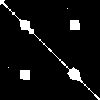
\includegraphics[width=\textwidth]{figures/method1/newtoy/newpost_sym2}
    \caption{connectivity computed using proposed MRF model}
    \label{fig:6dconn6}
    \end{subfigure}

    \caption[Test on synthetic data.]{Test of synthetic data by using
      correlation and MRF method proposed in this work. (a) Ground truth
      connectivity map. (b) Connectivity based on smoothed data. (c)
      Correlation of Gaussian-smoothed data. (d) Connectivity based on noisy
      correlations. (e) Connectivity based on smoothed data. (f) Connectivity
      computed using proposed MRF model. }
  \label{fig:6dconn}
\end{figure}


\begin{figure}[p] 
  \centering 
  \begin{subfigure}[t]{0.3\textwidth}
    \centering
    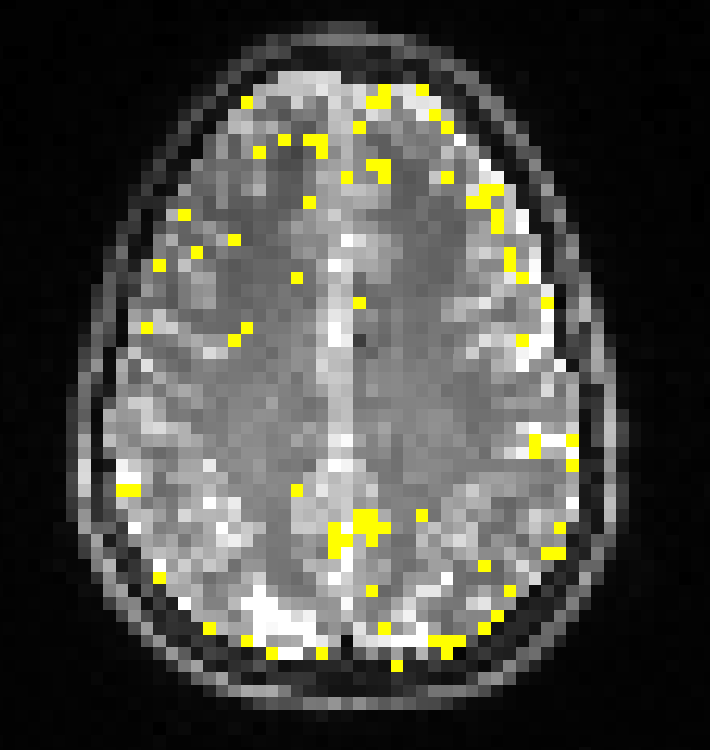
\includegraphics[width=\textwidth]{figures/method1/invivo1/r1}
    \caption{Sub1: correlation map without smoothing.}
    \label{fig:invivo11}
    \end{subfigure}
~
  \begin{subfigure}[t]{0.3\textwidth}
    \centering
    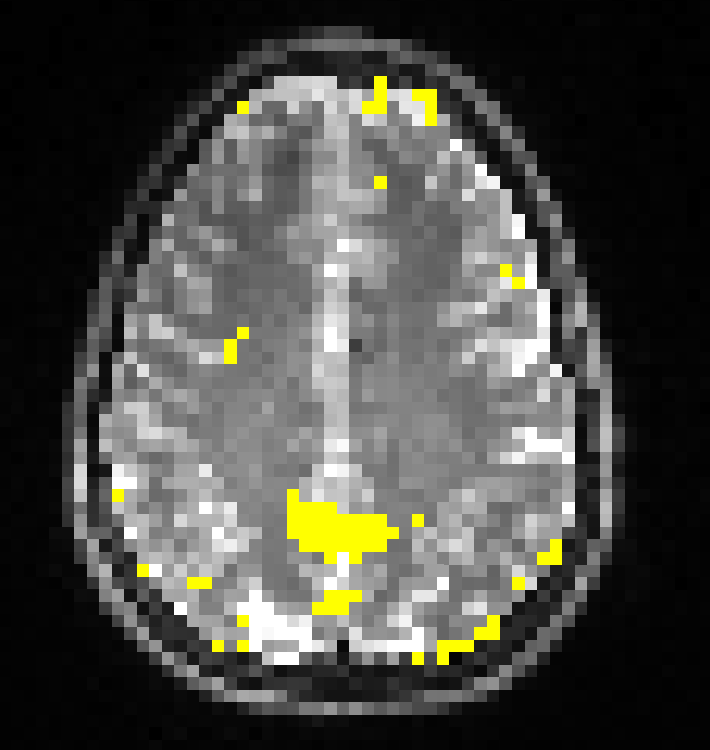
\includegraphics[width=\textwidth]{figures/method1/invivo1/r1_smooth}
    \caption{Sub1: correlation map with smoothing.}
    \label{fig:invivo12}
    \end{subfigure}
~
  \begin{subfigure}[t]{0.3\textwidth}
    \centering
    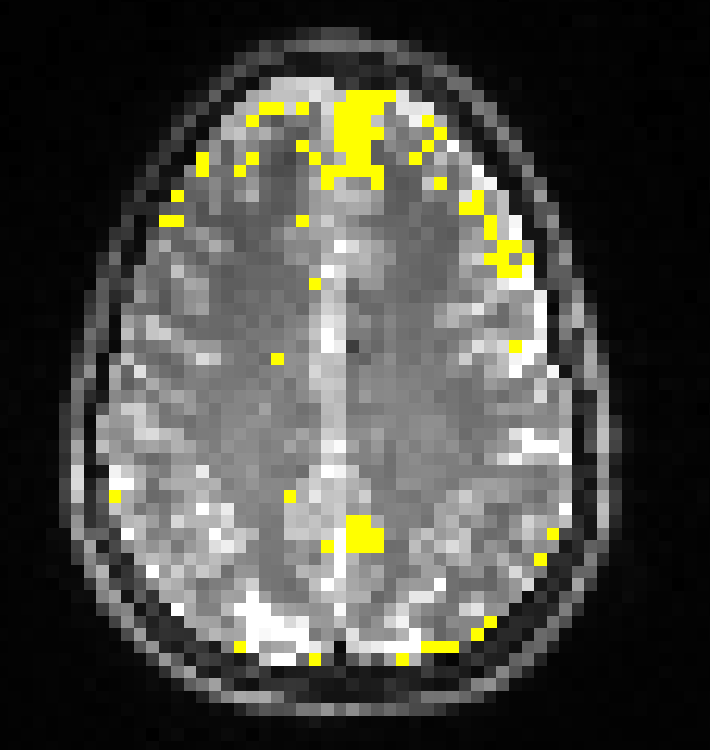
\includegraphics[width=\textwidth]{figures/method1/invivo1/r1_mrf}
    \caption{Sub1: posterior probability by MRF.}
    \label{fig:invivo13}
    \end{subfigure}

  \begin{subfigure}[t]{0.3\textwidth}
    \centering
    \includegraphics[width=\textwidth]{figures/method1/invivo1/r2}
    \caption{Sub2: correlation map without smoothing.}
    \label{fig:invivo14}
    \end{subfigure}
~
  \begin{subfigure}[t]{0.3\textwidth}
    \centering
    \includegraphics[width=\textwidth]{figures/method1/invivo1/r2_smooth}
    \caption{Sub2: correlation map with smoothing. }
    \label{fig:invivo15}
    \end{subfigure}
~
  \begin{subfigure}[t]{0.3\textwidth}
    \centering
    \includegraphics[width=\textwidth]{figures/method1/invivo1/r2_mrf}
    \caption{Sub3: posterior probability by MRF.}
    \label{fig:invivo16}
    \end{subfigure}
    \caption{ Threshold correlation mapand Posterior Connectivity map between
      seed voxel and the current slice, overlaid to T2 image.  (a) Subject 1:
      correlation without smoothing. (b) Subject 1: correlation with
      smoothing. (c) Subject 1: posterior estimated from MRF. (d) Subject 2:
      correlation without smoothing. (e) Correlation without smoothing. (f)
      Posterior estimated from MRF. }
  \label{fig:invivo1}
\end{figure}

\begin{figure}[p] 
  \centering 
  \begin{subfigure}[t]{0.3\textwidth}
    \centering
    \includegraphics[width=\textwidth]{figures/method1/invivo2/R1_corr_nosmooth}
    \caption{sub1: correlation without smoothing}
    \label{fig:invivo21}
    \end{subfigure}
~
  \begin{subfigure}[t]{0.3\textwidth}
    \centering
    \includegraphics[width=\textwidth]{figures/method1/invivo2/R1_corr_smooth}
    \caption{sub1: Correlation with smoothing}
    \label{fig:invivo22}
    \end{subfigure}
~
  \begin{subfigure}[t]{0.3\textwidth}
    \centering
    \includegraphics[width=\textwidth]{figures/method1/invivo2/R1_mrf}
    \caption{Posterior from MRF}
    \label{fig:invivo23}
    \end{subfigure}

  \begin{subfigure}[t]{0.3\textwidth}
    \centering
    \includegraphics[width=\textwidth]{figures/method1/invivo2/R2_corr_nosmooth}
    \caption{sub2: correlation without smoothing.}
    \label{fig:invivo24}
    \end{subfigure}
~
  \begin{subfigure}[t]{0.3\textwidth}
    \centering
    \includegraphics[width=\textwidth]{figures/method1/invivo2/R2_corr_smooth}
    \caption{sub2: correlation with smoothing.}
    \label{fig:invivo25}
    \end{subfigure}
~
  \begin{subfigure}[t]{0.3\textwidth}
    \centering
    \includegraphics[width=\textwidth]{figures/method1/invivo2/R2_mrf}
    \caption{sub2: posterior from MRF}
    \label{fig:invivo26}
    \end{subfigure}
  \caption{Correlation map and posterior connectivity map between seed voxel and
    slice containing the seed. (a) Subject 1: correlation without
    smoothing. (b) Subject 1: correlation with smoothing. (c) Subject 1:
    posterior estimated from MRF. (d) Subject 2: correlation without
    smoothing. (e) Correlation without smoothing. (f) Posterior estimated
    from MRF. }
  \label{fig:invivo2}
\end{figure}


%%% Local Variables: 
%%% TeX-master: "MyThesis"
%%% End: 

\chapter{Consistent and Spatially Coherent Functional Networks}
\label{chap:method2}
The pairwise functional connectivity estimation method in Chapter
\ref{chap:method1} estimates the connections between each pair of voxels, and
outputs a symmetric matrix with element $(i,j)$, the connectivity of voxel $i$ and
$j$. However, in order to explore  functional networks, we still need a
seed. Moreover, only those regions connected to the selected seed region can be
identified. If a seed is incorrectly chosen, it may fall outside of the
functional networks that we are interested in, the resulting network map will
not be informative. In this chapter, we propose a new data-driven method to
partition the brain's gray matter into disjoint partitions of functional
networks. Unlike the previous chapter, the proposed algorithm does not require
specification of a seed, and there is no ad hoc thresholding or parameter
selection. The algorithm identifies all of the functional network maps in a single
run. To achieve the above properties, we define the model in the original image
space and cluster the voxels with higher connectivity into the same class. This
is indeed an image segmentation problem, or an unsupervised clustering problem
in data mining. The proposed approach is, in spirit, similar to the functional
parcellation work that has been proposed by Yeo et
al.~\cite{yeo2011organization}.

We make a natural assumption that functionally homogeneous regions should be
spatially coherent. Our method incorporates spatial information through a MRF
prior on voxel labels, which models the tendency of spatially-nearby voxels to
be within the same functional network. Here we use a MRF to model the network
label's spatial soft constraint, such that the network component maps are
spatially coherent with a piecewise constant labeling. 

The BOLD time course at each voxel is first normalized to zero mean and unit
norm, which results in data lying on a high-dimensional unit sphere. We then
model the normalized time-series data as a mixture of von Mises-Fisher (vMF)
distributions \cite{banerjee2006clustering}. Each component of the mixture model
corresponds to the distribution of time series from one functional
network. Solving for the parameters in this combinatorial model is intractable,
and we therefore use a MCEM algorithm, which approximates the expectation step
using Monte Carlo integration. The stochastic property of MCEM makes it possible
to explore a large solution space, therefore it performs better than a standard
mode approximation method such as iterated conditional modes (ICM). Finally, we
demonstrate on real fMRI data that our method is able to identify visual, motor,
salience, and default mode networks with considerable consistency between
subjects.

The vMF distribution was first introduced in the machine learning community by Banerjee et
al.~\cite{banerjee2006clustering} to address the parametric clustering problem on
the dataset of documents. In such data, the similarity of two data samples is
better represented by the inner product of normalized feature vectors. By
normalization, the feature vector has zero mean and unit variance, which is
equivalent to being projected onto  a high-dimensional sphere. Original usage
of the inner product as distance metric is by Dhillon and Modha's
\textsf{spkmeans} algorithm~\cite{dhillon2001efficient}, where the cosine
similarity is used for clustering. When the features have high dimensions, the
\textsf{spkmeans} is superior to standard K-Means algorithm in terms of speed
and classification accuracy. The extension of \textsf{spkmeans} to
vMF~\cite{banerjee2006clustering} is similar to the extension of Gaussian
mixture model to the standard K-Means, except that vMF has a simplified
definition of variance (or, precision) such that the distribution is
isotropic. The vMF distribution is indeed a generalization of the lower
dimensional von Mises distribution, which is discussed by
Mardia~\cite{mardia2000directional} in the context of directional statistics.

\section {Hidden Markov models of functional networks}\label{sec:models}
% Bayesian, prior, likelihood
We use a Bayesian statistical framework to identify functional networks of the
gray matter in fMRI data. We formulate a generative model, which first generates
a spatial configuration of functional networks in the brain, followed by an fMRI
time series for each voxel based on its network membership. We employ an MRF
prior to model network configurations, represented by the hidden network label
variables. Given a label, we assume that the fMRI time series, normalized to
zero mean and unit norm, are drawn from a von Mises-Fisher distribution.

% notation: indices, labels
Let $\cV$ be the set of indices for all gray-matter voxels. We assume that the
number of networks $L$ is a known free parameter. Let $\cL = \{1, 2, \cdots,
L\}$ be the set of labels, one for each network. We denote a label map for
functionally-connected networks as a vector $X = (x_1,\dots, x_N), x_s \in
\cL$.  Let $\cX = \cL^N$ be the set of all possible $X$'s configurations.

\subsection{A Markov prior model}
Functional networks should consist of few, reasonably-sized, possibly distant
regions. We model such networks $X$ using a special case of MRF model that we
discussed in Chapter \ref{chap:math}, i.e., the Potts~\cite{li_markov_2009}:
\begin{equation*}
  P(X)  =  \frac {1} {Z} \exp \left \{ -\beta \sum_{(r,s)\in \cE}\psi(x_r, x_s) \right \},
\end{equation*}
where the function $\psi$ takes $1$ if its argument is not equal and $0$
otherwise; $(r,s)$ is the set of voxel pairs that are spatial neighbors on the
graph; $\beta > 0$ is a model parameter controlling the strength of label-map
smoothness; $Z$ is a normalization constant that is the sum of $P(X)$ over
all possible configuration of $X$. The Markov-Gibbs
equivalence~\cite{li_markov_2009} implies that the conditional distribution of $x_s$ at
site $s$ is:
\begin{equation}
  \label{eq:mrfprior}
  P(x_s | X_{-s})  = P(x_s | X_{\cN_s}) =  \frac {
    \exp \left\{ -\beta \sum_{r \in \cN_s} \psi(x_s, x_r) \right\}
  }
  {
    \sum_{l \in \cL} \exp \left \{ -\beta \sum_{r \in \cN_s} \psi(x_r, l) \right\}
  },
\end{equation}
where $X_{-s}$ is the collection of all variables in $X$ excluding
site $s$. The neighborhood is the usual six adjacent voxels, which does not overly
smooth across boundaries. Previous works
\cite{wei1990monte,descombes_spatio-temporal_1998} have demonstrated the
advantages of MRFs over Gaussian smoothing in preserving segment boundaries.

\subsection {Likelihood model}
% normalization
We observe that in order to make the analysis robust to shifts or scalings of
the data, one typically normalizes the time series at each voxel to zero mean and
unit length. This results in the data being projected onto a high-dimensional
unit sphere. After normalization, the sample correlation between two time series
is equal to their inner product, or equivalently, the cosine of the geodesic
distance between these two points on the sphere. Thus, we reformulate the
problem of finding clusters of voxels with high correlations to the problem of
finding clusters with small within-cluster distances on the sphere. Figure
\ref{fig:vmfdata} shows this equivalence.


% likelihood
In the previous chapter, the observed data are the linear correlations between a
prior of voxels BOLD signal. Since the correlation is a scalar, the emission
function, i.e., the conditional probability of $P(Y | X)$ can be easily modeled
by the Gaussian distribution once the correlation has been
Fisher-transformed. In the model of this chapter, the observed data are the BOLD
signal itself, so we need a multivariate distribution to model its conditional
probability.  We use the notation $Y = \{ (y_1, \dots, y_N)\, |\, y_s \in
S^{p-1} \}$ to denote the set of \emph{normalized} time series. Observe that
given $X \in \cX$, the random vectors $ y_s, \forall s \in \cV$ are conditional
independent. Thus, the likelihood $\log P(Y | X) = \sum_{s \in \cV} \log P (Y_s
| x_s)$. We model the emission function $P(y_s | x_s)$ using the von
Mises-Fisher (vMF) distribution
\begin{equation}
  f ( y_s;\mu_l, \kappa_l | x_s = l)  = C_p(\kappa_l)
  \exp (\kappa_l \mu_l^{\top} y_s),
  \quad   y_s \in S^{p-1}, \quad l \in {\cL}.
  \label{eq:vmf}
\end{equation}
For the cluster labeled $l$, $\mu_l$ is the mean direction, $\kappa_l \geq 0$ is
the \emph{concentration parameter}, and the normalization constant $C_p(\kappa)$ is given by 
\begin{equation*}
C_p(\kappa) = \frac{\kappa^{\frac{p}{2} - 1}}{((2\pi)^{\frac{p}{2}} I_{\frac{p}{2}-1}(\kappa))},
\end{equation*}
where $I_\nu$ denotes the modified Bessel function of the first kind with order
$\nu$. The larger the $\kappa$, the greater is the density concentrated around
the mean direction. When $\kappa = 0$, $f(y_s; \mu, \kappa)$ reduces to the
uniform distribution on $S^{p-1}$. If $\kappa \rightarrow \inf$, $y_s$ will be
in a point density.  Since \eqref{eq:vmf} depends on $y$ only by $\mu^{\top} y$,
the vMF distribution is unimodal and rotationally symmetric around $\mu$.

% 'prior' on kappa
In the Bayesian framework, we also define distributions on parameters. We assume
that $\forall l \in \cL$, $\kappa_l \sim \cN(\mu_{\kappa}, \sigma_{\kappa}^2)$
with hyperparameters $\mu_{\kappa}$ and $\sigma_{\kappa}^2$ that can be set
empirically. This prior enforces constraints that the clusters should not have
extremely high or low concentration parameters. We empirically tune the
hyperparameters $\mu_{\kappa}$ and $\sigma_{\kappa}^2$ and have found the
results to be robust to specific choices of the hyperparameters.

\subsection{Monte Carlo EM}
\label{sec:mcem}


The model of the functional network variables can be illustrated by Figure
\ref{fig:genevmf}. Given the definition of the prior and likelihood function, our
goal is the statistical inference of the posterior probability of $X$ given the
observed data $y$. Because of both the hidden variables $X$ and the model
parameters $\mu, \kappa, \beta$ are unknown, we use EM method to estimate them
in an iterative way.  To estimate the model parameters and the hidden labels, we
use the MCEM~\cite{wei1990monte} algorithm. The standard EM algorithm maximizes
the expectation of the log-likelihood of joint PDF of $Y$ and the hidden
variable $X$ with respect to the posterior probability $P(X | Y)$,
i.e., $\mathbb{E}_{P(X| Y)} [\log P(X, Y; \vec \theta)]$. The combinatorial
number of configurations for $X$ makes this expectation intractable. Thus, we
use Monte Carlo simulation to approximate this expectation as
\begin{equation}
  \widetilde Q(\vec \theta; X, Y)
  \approx
  \frac
  {1}
  {M}
  \sum_{m=1}^{M}
    \log
    P (X^m; \beta)
    +
    \log
    P (Y | X^m; \vec \theta_L),
  \label{eq:mcemq}
\end{equation}
where $X^m$ is a sample from $P(X | Y)$, $\vec \theta_L = \{\mu_l, \kappa_l : l
\in \cL\}$ is the parameter vector of the likelihood, and $\vec \theta=\{\beta,
\vec \theta_L\}$ is the full parameter vector of the model. Computing the MRF
prior in \eqref{eq:mcemq} is still intractable due to the normalization
constant, and we instead use a pseudo-likelihood approximation~\cite{li_markov_2009},
which gives
\begin{align*}
\centering
  \widetilde Q
  &
  \approx
  \frac{1}{M}
  \sum_{m=1}^{M}
  \sum_{s \in \cV}
  \log P(x_s | x_{\cN_s}; \beta)
  +
  \frac{1}{M}
  \sum_{m=1}^{M}
  \sum_{s \in \cV}
  \log
  P( y_s | x_s; \vec \theta_L)
  =
  \widetilde Q_P
  +
  \widetilde Q_L.
\end{align*}
We use $\widetilde Q_P$ to denote the log-pseudo-likelihood of the prior
distribution, and use $\widetilde Q_L$ to denote the log-likelihood
distribution. Now the prior term $\widetilde Q_P$ is in a tractable form for
evaluation, and we can estimate $\beta$ by optimization of $\widetilde Q_P$ with
a Newton-Raphson method, initialized by $\beta = 0$.  Because of the separation
of the parameters in $\widetilde Q_P$ and $\widetilde Q_L$, we can estimate the
parameter $\vec \theta_L$ by optimizing $Q_L$. There is an approximated closed
form solution for this estimation, and we will discuss it in Section
\ref{sec:thetal}.

\subsection{Sampling from the posterior}
Given the observed data $Y$ and parameter value $\vec \theta =
\{\beta, \vec \theta_L \}$, we sample from the posterior
distribution $P(X | Y; \vec \theta)$ using Metropolis
sampling. We define the posterior energy, which is to be minimized, as the
negative log of the posterior $P(x_s | Y_s)$. Thus,
Bayesian rule implies:
\begin{equation}
  U( x_s = l| X)
  =
   \beta \sum_{r \in \cN_s} \psi(x_s, x_r) - \log C_p(\kappa_l)
    -
    \kappa_l \mu_l^{\top}  y_s
  + \mathrm{const},
  \label{eq:sample}
\end{equation}
which is the sum of the prior energy, the conditional energy, and a
parameter-independent quantity. Then, given a current configuration $X^m$,
Metropolis sampling generates a new candidate label map $\vec w$ as follows: (i)
Draw a new label $l'$ at site $s$ with uniform distribution; $W$ has value $l'$
at site $s$, with other sites remaining the same as $X^m$; (ii) compute the
change of energy $\Delta U(W) = U(W | Y) - U( X^m | Y) = U(x_s = l'| Y) - U(x_s
= l | Y)$; (iii) accept candidate $W$ as $X^{m+1}$ with probability $\min
(1, \exp \{ -\Delta U(W) \})$; (iv) after a sufficiently long burn-in
period, generate a sample of size $M$ from the posterior distribution $P(X|
Y)$. This is indeed the Metropolis sampling algorithm (Algorithm~\ref{alg:metro}) that
we have introduced in Chapter \ref{chap:math}.

\subsection{Parameter estimation}
\label{sec:thetal}
In order to estimate $\mu$ and $\kappa$ of the vMF distribution, we need to
maximize $\widetilde Q_L$ with the constraint $\norm{\mu_l} = 1$ and
$\kappa > 0$. For one sample label map, the maximum likelihood maximization of
the mean vector $\mu_l$ for label $l$ is~\cite{banerjee2006clustering,
  dhillon2003modeling}
\begin{align}
  \mu_l &= \argmax_{\mu_l} \prod_{s\in \cV_l} P(y_s; \mu_l, \kappa_l | X) \nonumber\\
  &= \argmax_{\mu_l} \sum_{s\in \cV_l} \log P(y_s; \mu_l, \kappa_l | X) \nonumber\\
  &= \argmax_{\mu_l} \sum_{s\in \cV_l} N \log C_p(\kappa_l) + \kappa_l \mu_l^{\top} R_l, 
  \label{eq:estmu}
\end{align}
where $\cV_l = \{ s \in \cV: x_s = l\}$ is the set of data points in cluster
$l$, and $R_l = \sum_{s \in \cV_l}^{} y_s$. We maximize \eqref{eq:estmu} with
the constraints $\mu_l^{\top} \mu$ by introducing a Lagrangian multiplier and obtain
\begin{equation}
  \hat \mu_l = R / \| R_l \|.
\end{equation}

In MCEM, instead of having one label map, we have $M$ maps sampled from
$P(X|Y)$. The $M$ sample maps are not independent since they were obtained in a
consecutive time point. But for the purpose of parameter estimation, we can
safely assume the independence and pool them into same dataset, where we extract
the subset of label $l$ to estimate $\mu_l$. We can estimate $\mu$ as
\begin{equation}
  R_l = \sum_{m=1}^{M}\sum_{s \in \cV_l}^{} y_s, \qquad \hat {\mu}_l = \frac{R_l}{\norm{R_l}},
  \label{eq:mlmu}
\end{equation}
We have no \emph{a priori} knowledge for $\mu_l$, so a maximum likelihood
estimation in \eqref{eq:mlmu} is the best we can do. For $\kappa_l$ we maximize
the posterior distribution $P(\kappa_l | Y, X^1, \dots, X^M) $.  Since
$\widetilde Q_P$ is not dependent on $\kappa$, we maximize $\widetilde
Q_L(\kappa_l) + \log P(\kappa_l; \mu_{\kappa}, \sigma_{\kappa}^2)$ and
get~\cite{banerjee2006clustering}
\begin{equation}
  A_p(\hat \kappa_l) + \frac{\hat \kappa_l - \mu_{\kappa}}{N_l\sigma_{\kappa}^2} = R_l,
  \label{eq:estkappa}
\end{equation}
where $A_p(\hat \kappa_l) = I_{\frac{p}{2}} (\hat \kappa_l) / I_{\frac{p}{2}-1}
(\hat \kappa_l)$ and $N_l = |\cV_l|$ is the number of data points in cluster
$l$. Because \eqref{eq:estkappa} contains the ratio of two modified Bessel
functions, an analytic solution is unavailable and we have to resort to a
numerical solution. We use Newton's method for solving $g(\hat \kappa_l) =
A_p(\hat \kappa_l) -(\hat \kappa_l - \mu_{\kappa}) / (N_l\sigma_{\kappa}^2) -
R_l= 0$. The choice of initial value for Newton's algorithm depends on the
strength of the prior on $\kappa_l$ (i.e., the $\sigma_{\kappa}$ value). For a
noninformative prior, $\hat \kappa_l = (pR_l - R^3) / (1 - R^2)$ is a good a
good initial value \cite{banerjee2006clustering}. For a strong prior, a
reasonable initial value is the current value of $\kappa_l$.

To estimate $\beta$, we again rely on Newton's method to find the solution
numerically. The derivatives $\partial \widetilde Q_P / \partial \beta$ and
$\partial^2 \widetilde Q_P / \partial \beta^2$ for the pseudo-likelihood
approximation of the MRF prior are easily computed. With all the settings above,
we give the steps of the E step and M step iterations in
Algorithm~\ref{alg:mcem}.


\begin{algorithm}[p]
  % \DontPrintSemicolon
  \SetKwInOut{Input}{input}\SetKwInOut{Output}{output}
  \Input{Preprocessed 4D fMRI data; number of clusters}
  \Output{Labeled functional network map}

  Initialization: Run $k$-means clustering a few times and choose $\mat z$ with the smallest sum-of-square errors; estimate $\vec \theta_L$ and set
  $\beta$ to a small value\;

  \While{MCEM not converged}{
    \textbf{E step: } Given current $\vec \theta$,
    \For{$m \leftarrow 1$ \KwTo $M$}{
      \lForEach{$s \in \cV$} {
        Draw sample $x_s^m$ from $P( x_s|Y_s)$ using \eqref{eq:sample}\;
      }
    }
    \textbf{M step: } Given $(X^1,\dots, X^M)$, estimate $\beta$ and $\vec \theta_L$\;
    Estimate labels with ICM  using the current estimates for $\beta$ and $\vec \theta_L$ \;
  }
  \caption{MCEM-ICM Algorithm for Hidden-MRF Model Estimation}
  \label{alg:mcem}
\end{algorithm}



Given the methods for sampling and parameter estimation, we estimated the
hidden MRF model by iteratively using (i) MCEM to learn model parameters and
(ii) using ICM to compute optimal network labels. In the expectation (E) step,
we draw samples from the posterior $P(X | Y)$, given current estimates
for parameters $\vec \theta$. In the maximization (M) step, we use these samples
to update estimates for the parameters $\vec \theta$.

\section{Experiment results}
\label{sec:exp}

In this section, we give preliminary test results on simulated fMRI dataset,
in order to show its accuracy under large noise. We then apply our MCEM method
on the \emph{in vivo} data.

\subsection{Synthetic data}
We first simulate low-dimensional time series (two-dimensional 64$\times$64
image domain; three time points, for visualization on sphere $S^2$) to compare
the (i)~proposed method using MCEM with (ii)~the mode-approximation approach
that replaces the E step in EM with a mode approximation. We simulate a label
map by sampling from a MRF having $\beta = 2$ and number of labels
$L=4$. Given the label map, we simulate vMF samples on the sphere $S^2$. The
method we used to simulate samples from vMF distribution is from
Dhillon~\cite{dhillon2003modeling} and
Wood~\cite{wood1994simulation}. Figure~\ref{fig:toy} gives the simulated data
and the estimation by the two methods. We note the simulated network label map
is piecewise constant, with occasional small regions scattered between large
patches. This is similar to the estimated functional network maps from the
real data. Although there are only three time points, it is difficult to
visualize the dynamic change of the voxel intensity over time, so we choose to
show only the volume at the first time point on the second image of
Figure~\ref{fig:toy}. Both the ICM and MCEM model are initialized with a
K-Means clustering. We observe that ICM easily converges to a local minimum of
the energy function within a few iterations, and its estimated labels are less
accurate compared with our MCEM approach. The MCEM solution is close to the
ground truth, while the mode-approximation solution is stuck in a local
maximum.



\subsection{Real rs-fMRI} 
We evaluated the proposed method on real data obtained from healthy control
subjects, in a resting-state fMRI study. BOLD EPI images (TR = 2.0 s, TE = 28
ms, 40 slices at 3 mm slice thickness, 64 x 64 matrix, 240 volumes) were
acquired on a Siemens 3 Tesla Trio scanner. The data was preprocessed in SPM,
including motion correction, registration to T2 and T1 structural MR images,
spatial smoothing by a Gaussian filter, and masked to include only the
gray-matter voxels. We used the \texttt{conn}
software to regress out signals
from the ventricles and white matter, which have a high degree of physiological
artifacts. A bandpass filter was used to remove frequency components below 0.01
Hz and above 0.1 Hz. We then projected the data onto the unit sphere by
subtracting the mean of each time series and dividing by the magnitude of the
resulting time series. We then applied the proposed method to estimate the
functional network labels with the number of clusters set to $L = 8$.

Figure~\ref{fig:wholebrain} shows the optimal label maps, produced by the
proposed method for 3 of all 16 subjects in the dataset. We note that among the
eight clusters, one cluster, with the largest $\kappa$ value and largest number of
voxels, corresponds to background regions with the weakest connectivity and is not
shown in the figure. Among the clusters shown, we can identify the visual,
motor, dorsal attention, executive control, salience, and default mode networks
(DMN)~\cite{raichle2001default}. Four networks: the visual, motor, executive control,
and DMN, were robustly found across all subjects. More variability was found in
the dorsal attention network (notice that it is much larger in subject 3) and
salience network (notice that it is missing in subject 2). We found that
changing the number of clusters, although leading to different label maps,
preserves the four robust networks. For instance, we also ran the analysis with
the number of clusters set to 4 or 6 (results not shown) and were able to
recover the same four robust networks.



\begin{table}[p]
  \centering
  \caption{The number of voxels with value greater than 8 in the overlapped label map. }
  \begin{tabular*}{0.75\textwidth}{@{\extracolsep{\fill}} l  r r r r}
    & DMN & Motor & Attention & Visual \\
    \hline
    MCEM    & 5043  & 7003 & 3731 & 5844 \\
    Individual ICA & 114 & 167 & 228 & 134 \\
    Group ICA & 3075 & 5314 & 3901 & 3509 \\
    \hline
  \end{tabular*}\label{table:agreement}
\end{table}

The next experiment compares our results with ICA. A standard ICA toolbox (GIFT;
\url{mialab.mrn.org}) was applied on the same preprocessed data of each subject
independently, which we call ``Individual ICA''. We also applied standard Group
ICA, using all data from the 16 subjects simultaneously. In both ICA experiments
the number of components are set to 16. The component maps are converted to z
score and thresholded at 1. For each method we computed an overlap map for each
functional network by adding the corresponding binary label maps of all 16 subjects.
The results in Figure~\ref{fig:multisub} show our method can detect the motor,
attention, and visual network with accuracy comparable with Group ICA. Besides,
our method also detects DMN with posterior cingulate cortex (PCC) and medial
prefrontal cortex (MPFC), while Group ICA split the DMN into two components, one
with the MPFC and another with the PCC (not shown).

To see the consistency of the label map between subjects for all three methods,
we look at each method's overlapped label map and count the number of voxels
whose value are greater than 8. Table~\ref{table:agreement} shows that our
method exhibits better consistency than both Individual and Group ICA.


\section{Discussion}
We proposed a segmentation algorithm and applied it on single subject rs-fMRI
data. The output of the algorithm is a label map, in which voxels of the same
functional network are assigned the same labels. The label of each voxel has a
spatial dependency on its neighbors, and we use a MRF to model the
interdependency, and accordingly define a prior distribution of the label
map. The posterior inference is an intractable problem due to the complex
dependency of multiple variables. We use MCEM to draw samples from the
posterior distribution and use the samples for parameter estimation. The
Metropolis sampling uses a uniform distribution as a proposal
distribution. Because there are $L$ possible labels in this uniform
distribution, there is a higher chance that the uniform does not propose the
best label value during the first few  scans. When $L$ is large, we
accordingly need more scans for the proposal distribution to catch the best
label. Therefore, the burn-in times are longer than the binary case in Chapter
\ref{chap:method1}.

\begin{figure}[p] 
  \centering 
  \begin{subfigure}[t]{0.3\textwidth}
    \centering
    \includegraphics[width=\textwidth]{figures/method2/vmf}
    \caption{Two vectors on 1-D sphere.}
    \label{fig:vmf}
    \end{subfigure}
~
  \begin{subfigure}[t]{0.3\textwidth}
    \centering
    \includegraphics[width=\textwidth]{figures/method2/sphere1}
    \caption{time series data on high-D sphere.}
    \label{fig:sphere}
    \end{subfigure}
  \caption{Data points with Von Mises-Fisher distribution.}
  \label{fig:vmfdata}
\end{figure}

\begin{figure}[p] 
  \centering
  \includegraphics[width=0.5\textwidth]{figures/method2/genevmf}
  \caption{A generative model of the functional network. The network variable
    $X$ is a multivariate variable defined on a MRF. Given $X$, $Y$ is seen
    as being generated from a vMF distribution whose parameter $\mu$ and
    $\kappa$ are functions of $X$.}
  \label{fig:genevmf}
\end{figure}

\begin{figure}[p]
  \centering

  \centering 
  \begin{subfigure}[b]{0.19\textwidth}
  \includegraphics[width=1\textwidth]{figures/method2/synthetic/true}
  \caption{Observed noise image}
  \end{subfigure}
~
  \begin{subfigure}[b]{0.19\textwidth}
  \includegraphics[width=1\textwidth]{figures/method2/synthetic/obs}
  \caption{Observed noise image}
  \end{subfigure}
~
  \begin{subfigure}[b]{0.19\textwidth}
  \includegraphics[width=1\textwidth]{figures/method2/synthetic/label_icm}
  \caption{Observed noise image}
  \end{subfigure}
~
  \begin{subfigure}[b]{0.19\textwidth}
  \includegraphics[width=1\textwidth]{figures/method2/synthetic/label_mc}
  \caption{Observed noise image}
  \end{subfigure}

  \caption{Synthetic example. (a) True labels, (b) First time point of
    observed time series, (c) Time series plot on sphere, (d) Label map
    estimated by mode-approximation, and label map estimated by MCEM.}
  \label{fig:toy}
\end{figure}

\begin{figure}[p]
  \centering
  \includegraphics[width=0.15\textwidth]{figures/method2/wholebrain/sub1/axial0028} 
  \includegraphics[width=0.15\textwidth]{figures/method2/wholebrain/sub1/axial0034} 
  \includegraphics[width=0.15\textwidth]{figures/method2/wholebrain/sub1/saggital0029} 
  \includegraphics[width=0.15\textwidth]{figures/method2/wholebrain/sub1/coronal0029} \\

  \includegraphics[width=0.15\textwidth]{figures/method2/wholebrain/sub2/axial0028} 
  \includegraphics[width=0.15\textwidth]{figures/method2/wholebrain/sub2/axial0034} 
  \includegraphics[width=0.15\textwidth]{figures/method2/wholebrain/sub2/saggital0029} 
  \includegraphics[width=0.15\textwidth]{figures/method2/wholebrain/sub2/coronal0029} \\

  \includegraphics[width=0.15\textwidth]{figures/method2/wholebrain/sub5/axial0028} 
  \includegraphics[width=0.15\textwidth]{figures/method2/wholebrain/sub5/axial0034} 
  \includegraphics[width=0.15\textwidth]{figures/method2/wholebrain/sub5/saggital0029} 
  \includegraphics[width=0.15\textwidth]{figures/method2/wholebrain/sub5/coronal0029}
  \caption {Functional networks detected by the proposed method for 3 subjects
    overlaid on their T1 images.  The clusters are the visual (cyan), motor
    (green), executive control (blue), salience (magenta), dorsal attention
    (yellow), and default mode (red) networks.}
  \label{fig:wholebrain}
\end{figure}

\begin{figure}[p]
  \centering
  \begin{subfigure}[b]{1\textwidth}
    \centering
    MCEM \hspace{2cm}single subject ICA \hspace{2cm}group ICA. 

    \end{subfigure}

  \begin{subfigure}[b]{1\textwidth}
    \centering
      \includegraphics[height=0.14\textwidth]{figures/method2/mcem/dmn_a} 
      \includegraphics[height=0.14\textwidth]{figures/method2/mcem/dmn_s} 
      \includegraphics[height=0.14\textwidth]{figures/method2/ica_separate/DMN_a} 
      \includegraphics[height=0.14\textwidth]{figures/method2/ica_separate/DMN_s}
      \includegraphics[height=0.14\textwidth]{figures/method2/ica_single/dmn_a} 
      \includegraphics[height=0.14\textwidth]{figures/method2/ica_single/dmn_s} 
      \caption{}
      \label{fig:mcemdmn}
  \end{subfigure}

  \begin{subfigure}[b]{\textwidth}
    \centering
    \includegraphics[height=0.14\textwidth]{figures/method2/mcem/motor_a} 
    \includegraphics[height=0.14\textwidth]{figures/method2/mcem/motor_s} 
    \includegraphics[height=0.14\textwidth]{figures/method2/ica_separate/motor_a} 
    \includegraphics[height=0.14\textwidth]{figures/method2/ica_separate/motor_s}
    \includegraphics[height=0.14\textwidth]{figures/method2/ica_single/motor_a} 
    \includegraphics[height=0.14\textwidth]{figures/method2/ica_single/motor_s} 
    \caption{}
    \label{fig:mcemmotor}
  \end{subfigure}

  \begin{subfigure}[b]{\textwidth}
    \centering
    \includegraphics[height=0.14\textwidth]{figures/method2/mcem/visual_a} 
    \includegraphics[height=0.14\textwidth]{figures/method2/mcem/visual_s} 
    \includegraphics[height=0.14\textwidth]{figures/method2/ica_separate/visual_a} 
    \includegraphics[height=0.14\textwidth]{figures/method2/ica_separate/visual_s}
    \includegraphics[height=0.14\textwidth]{figures/method2/ica_single/visual_a} 
    \includegraphics[height=0.14\textwidth]{figures/method2/ica_single/visual_s} 
    \caption{}
    \label{fig:mcemvisual}
  \end{subfigure}

  \begin{subfigure}[b]{\textwidth}
    \centering
    \includegraphics[height=0.14\textwidth]{figures/method2/mcem/atten_a} 
    \includegraphics[height=0.14\textwidth]{figures/method2/mcem/atten_s} 
    \includegraphics[height=0.14\textwidth]{figures/method2/ica_separate/atten_a} 
    \includegraphics[height=0.14\textwidth]{figures/method2/ica_separate/atten_s}
    \includegraphics[height=0.14\textwidth]{figures/method2/ica_single/atten_a} 
    \includegraphics[height=0.14\textwidth]{figures/method2/ica_single/atten_s} 
    \caption{}
    \label{fig:mcematten}
  \end{subfigure}
  \caption{Comparison of the overlap of the label maps estimated by our MCEM
    approach, group ICA and single subject ICA on 16 subjects.  Color map
    ranges from 8 (red) 16 (yellow). (a) MDN, (b) motor, (c) visual, (d)
    attentive.}
  \label{fig:multisub}
\end{figure}

%%% Local Variables: 
%%% TeX-master: "MyThesis"
%%% End: 

\chapter{Hierarchical Model For Group Analysis}
\label{chap:method3}
In this chapter, we will apply the graphical model and MRF to one of the core
problems in functional network analysis: estimation of networks from a group of
subjects. To study the brain's intrinsic activity with rs-fMRI data, one either
models the data of a single subject or a group of subjects. The BOLD signals of a single
subject are often contaminated with the noise of various sources, and the
results are typically unreliable for the inference of the whole population.  On
the other hand, combining data from multiple subjects and jointly estimating the
common functional networks is more robust. In group analysis of rs-fMRI one assumes
that all subjects in the group share common functional connectivity patterns and
that the group networks can be estimated more accurately because the noise
from each subject is canceled by averaging. In practice, it is a major challenge
to summarize the consistent patterns across subjects, as each subject's network
structure appears similar but has slight variations.

In this chapter we propose a Bayesian hierarchical model for estimating the
functional networks by using the rs-fMRI data from a group of subjects. The
hierarchy comes from an additional level of \emph{group} map defined on top of
the conventional subject functional network maps. The group effect goes into the
subject network label's probabilistic distribution as a parameter. Both group
and subject networks are jointly estimated in an iterative way. We give a
natural interpretation of the regularization with a Bayesian perspective. Once
the group's network map is known, it can help the individual subject's
estimation as a prior probability.  Because the group map combines the
information from all subject maps, this prior distribution is equivalent to
using other subjects' data for the current subject's inference.  Besides, a
subject's network estimates also help to iteratively refine the group map
estimates. We model the intersubject variability by balancing between a common
map for all subjects (no variability, maximal shared information) and a separate
map for each subject (no shared information, maximal variability). We achieve
the optimal balance in the Bayesian sense by computing the subject network
label's posterior density. This posterior density combines the prior information
from the group map and the data likelihood from the subject-specific BOLD
signal. We further model the within-subject spatial coherence by a Markov random
field (MRF). In the remaining part of the paper, we refer to our model a
\emph{hierarchical Markov random field} (HMRF).

A classical occurrence of hierarchical modeling in fMRI is the inclusion of
random effects in a general linear model (GLM)~\cite{beckmann2003general},
which is later extended to a full Bayesian
framework~\cite{woolrich2004multilevel}. The multilevel model has richer
structures and can capture the structures in multiple-group, multiple-session
data, and distinguish between the influence of the fixed effect and that of the
random factors. In our model, the hierarchy is defined on a latent variable
mixture representation.

A Markov random field is a multivariate distribution defined on an undirected
graph to represent the soft constraints between the variables. In fMRI analysis,
it is a principal regularization method of obtaining a spatially coherent
solution. Depending on the context, previous works have defined MRF on different
variables.  They have been used for the regularization priors on the
coefficients of the general linear model (GLM)~\cite{penny2005bayesian}, on the
parameters of a spatiotemporal auto-regression model~\cite{woolrich2004fully},
and on the hidden activation variables in task-based
experiments~\cite{hartvig2000spatial}. In this article, we define MRF on the
latent network label variables of hidden Markov model (HMM), to represent our
prior knowledge of the spatial coherence of the network patterns within a
subject. There is a key difference between our model and conventional HMMs,
though. We generalize the conventional concept of spatial regularization by
defining a \emph{joint} graph that includes the network variables of both the
group and subject levels. In our model, the neighbors of each node on the graph
include the corresponding nodes at another level, as well as the spatially
adjacent voxels in the same level. The new graph introduces our additional
assumption that one subject's functional networks should share similar patterns
with another subject's, implicitly represented by the group. With this
definition, we map all the variables in a hierarchical model on to a single
graph, and formulate a problem conceptually appealing and feasible in practice.

%% Optimization of MRF. Past method, our method. approximation.
The exact inference of MRF is a combinatorial optimization of discrete
variables, hence it is computationally infeasible except in special
cases~\cite{greig1989exact,ng2012modeling}. The iterated conditional mode (ICM)
is typically used to obtain a local optimum of the mode of the posterior
density~\cite{besag1986statistical}. In this work we are interested in the
posterior variance of the network label variables as well as the mode, and we
use MCEM sampling algorithm for the inference of both group and subject label
maps. MCEM is data-driven in that the model parameters are estimated together
with the network label variables. The only parameter that needs special
treatment is the link strength between the group and subjects. MCEM integrates
the Markov chain Monte Carlo sampling in the expectation-maximization loop. The
price to pay is the  longer computation time than in other approximate inference
methods such as variational Bayes.

We show our HMRF model is able to recover both group and subject functional
networks in simulated group fMRI data. While HMRF's group estimates are
comparable or more accurate than the two other methods under comparison, we are
especially interested in the higher accuracy of the individual subjects'
estimates. We further show the strength of the model by a real multiple-session
dataset, where we achieve significantly higher intersession consistency by using
our joint-estimation model. The method also proves to be more stable under the
data perturbation in a bootstrap experiment. This paper is based on our earlier
work~\cite{liu2012group}, and we extend previous work to redefine the model in
an integrated graphical model context. The new simulated data experiments
explore the performance of the algorithm under various levels of spatial
smoothing. In the real data experiments, we added a new intersession consistency
test and the algorithm stability test with bootstrapping. We also improved the
parameter estimation by using the Bayesian posterior predictive distribution of
the test subjects in a cross-validation framework.

In the remainder of this chapter, we define the model in Section
\ref{sec:m3model}, and give the approximate inference procedure in Section
\ref{sec:m3inference}. We compare the accuracy and consistency of our method,
together with other methods by testing on synthetic and real data experiments in
Section \ref{sec:synexperiments} and Section \ref{sec:realexperiments} and
discuss the model and algorithm performance in Section \ref{sec:discussion}.

\section{Related works}
\label{sec:ref}
ICA is a powerful tool for identifying functional networks by using rs-fMRI of
a single subject~\cite{calhoun2001spatial}. ICA is used to recover the
statistically independent functional components without \emph{a priori}
knowledge of the regions of interest. See Figure \ref{fig:c2ica} for how spatial
and temporal ICA methods are defined. Group ICA is used as an extension of
single-subject ICA in order to seek a set of independent components shared
across all subjects~\cite{calhoun2001spatial}. In a typical group ICA study, all
subjects are registered to a common atlas and assumed to share a common spatial
component map but have distinct time courses. The BOLD signals from all subjects
are concatenated temporally, followed by a single-subject ICA analysis. The
subject component maps are then obtained by a back-reconstruction
procedure. Alternatively, single-subject ICA is applied on each subject first,
and a self-organized clustering algorithm applies to all subjects' components
such that similar components are assigned into one cluster. The group ICA
components are represented by the centers of the
clusters~\cite{esposito2005independent}. Neither of the above approaches
iteratively refine group (or subject) maps once the subject (or group) maps are
estimated.

ICA as a signal decomposition method obtains overlapped spatial components and
needs ad-hoc thresholding. Such ambiguity makes interpreting the results
difficult. On the other hand, functional networks estimation can also be defined
as an image segmentation problem. The region-of-interest (ROI), or even the
whole brain voxels can be partitioned into disjoint spatial patches. The patches
with the same network labels, even when spatially remote from each other, belong
to the same functional networks. To extend the segmentation method to a group of
subjects, segmentations are performed first on individual subjects. The
connectivity maps are averaged to obtain a group affinity matrix. A second level
segmentation is performed on this affinity matrix~\cite{bellec2010multi,
  van2008normalized}. Again, subject network maps are not refined from the
estimates of the group network.

%% Need review papers: 'surface...' and show our work is different from theirs.
It is worth noting that Ng et al.~\cite{ng2012modeling} also use MRF for group
study. The spatial neighborhood is extended to cross-subject voxels, in order
to address the imperfect anatomical alignment and functional
correspondence. Our model is different from Ng's group MRF model in that 1) a
group level is defined in our model, whereas in Ng's work, a combined
structure including all subjects is defined without a group level. In such a
flat model, a voxel directly uses the information of the corresponding voxels
of other subjects. Instead, we expect a second level enriches the model and
better decomposes the fixed and random effects in the subject network map. 2)
Ng et al. define the MRF prior on the GLM coefficients in task-based
experiments so the posterior inference is a two-class problem (active versus
inactive), and an exact solution can be obtained by a graph-cuts
algorithm. Our model applies to the network labels in a rs-fMRI study, and
hence is a multiclass segmentation problem that is significantly more
difficult to solve. 3) The unary potential function in the model of Ng is
defined via the posterior probability of the label variable given the GLM's
coefficients, and there is no explicit splitting between the MRF prior and the
likelihood. This modeling method is essentially a conditional random
field~\cite{lafferty2001conditional}.  In our model, the unary potential in
the MRF prior is defined as the links between group and subject level, and
thus is separated from the data likelihood, so our model is a variant of the
hidden Markov model. Thanks to the Bayesian perspective of our hierarchical
model, the trade-off between prior and likelihood is accounted for
automatically. 4)The MRF model of Ng et al.  is built on certain regions of
the brain, while ours is built on the whole brain's gray matter voxels.

% Other related work.
Another class of methods identifies the functional spatial patterns by
decomposing the BOLD signal, which can be seen as generalizations of
ICA~\cite{varoquaux2010group,varoquaux2011multi} methods. The authors of both
works introduce generative models that include a population level and subject
level.  Each subject's mixing weight coefficients are regarded as being
generated from population level latent factors, and the population and subject
level's mixing matrices are solved jointly as a convex optimization
problem~\cite{varoquaux2011multi}. With regard to the joint estimation of both
levels of the hierarchy, we can see such methods as a counterpart of our model
in the class of signal decomposition methods.

\section{Hierarchical MRF For modeling group fMRI}
\label{sec:m3model}
We begin by defining each subject's network label map as a Markov random field
(MRF) with the neighborhood structure given by a regular lattice. The
statistical dependency between adjacent voxels acts as a prior model favoring
spatial coherence of estimated functional regions. To generalize the MRF to a
hierarchical setting, an additional group label map is defined in addition to
all subject label maps. The group label map has the same number of voxels and
the same Markov structure as the individuals' maps, again to encourage spatial
coherence of the functional regions in the group level. In addition, each voxel
in the group map is connected to the corresponding voxel in each subject
map. These connections model the relationships between the group and the
individuals. The subjects' functional network labels are regarded as generated
from the group labels, and the rs-fMRI time courses are regarded to be generated
from a mixture of high-dimensional distributions given the subject network
labels. All voxels of subjects and group label map are jointly connected into a
single MRF.  The functional network estimation is the inverse problem of the
above data generation process, as the labels are inferred from their posterior
distribution given the data. See Figure~\ref{fig:graphical} for an illustration.

More specifically, we follow the notation in Chapter \ref{chap:math} and define
an undirected graph $\cG = (\cV, \cE)$. The set of vertices $\cV = (\cV_G,
\cV_1, \cdots, \cV_J)$ is the union of the gray matter voxels $\cV_j$ for all
$J$ subjects as well as those in the group volume $\cV_G$.  An edge $(s, t) \in
\cE$ is defined in one of three types: (1) $s\in \cV_G, t\in \cV_j$ and $s$, $t$
have the same physical coordinates, (2) $s, t\in \cV_G$, and $s, t$ are spatial
neighbors, or (3) $s, t\in \cV_j$, and $s, t$ are spatial neighbors. In our
model we use a 26-neighbor system in a three-dimensional volume image (a voxel at the boundary
of the gray matter may have < 26 neighbors). We will refer to the first type of
link as \emph{between-level} links, and the second and third types of links as
\emph{within-subject links}. On each node $s \in \cV$, a discrete random
variable $x_s \in \cL = \{1,\cdots, L\}$ is defined to represent the functional
network label. We use $-s$ for the set of nodes excluding node $s$, and $\cN(s)$
for the set of neighboring nodes of $s$. Last we define clique $c$ as a complete
subgraph of $c $, such that every pair of nodes in $c$ has a link between them,
and define $\cC$ the set of all cliques in $\cG$.

\subsection{MRF prior}
\label{sec:mrfprior}
MRF is a principal regularization method for modeling spatial context
information. In a Bayesian setting, we use it as a prior distribution of the
network label variables $X = \{x_s \in \cL| s\in \cV \}$. Formally, with
the definition of the graph $\cG$ and neighbor system $\cN(s), \forall s \in
\cV$ above, $X$ is said to be a MRF on $\cG$ if $P(x_s | x_{-s}) = P(x_s |
x_{\cN(s)})$, i.e., a variable is conditional independent of the variables on the
remaining nodes of the graph given its neighbors~\cite{li_markov_2009}. This
local \emph{conditional independence} property is difficult to apply to the
inference of the joint distribution. Thanks to the equivalence of MRF and Gibbs
fields~\cite{besag_spatial_1974}, one can transform the local property into a
global property. A Gibbs random field or Gibbs distribution takes the form of
$P(X) = (1/Z) \exp\{ -U(X)\}$, where $Z$ is a normalization constant called
partition function in order to guarantee the function integrates to 1, and
$U(X) = \sum_{c\in \cC} V_c(X_c)$ is called the energy function. Each clique
potential function $V_c$ only depends on the variables in the corresponding
clique $c$. The Hammersley-clifford theorem~\cite{clifford1990markov} states
that $X$ is a MRF if and only if it obeys a Gibbs distribution. In this
specific problem, the energy function takes the following form:
\begin{align}
  U(X) &= \sum_{s,r\in\cV_G} \beta \psi(x_s, x_r) + \sum_{j=1}^J \left ( \sum_{s\in\cV_G, \tilde s\in\cV_j} \alpha \psi(x_s, x_{\tilde s}) + \sum_{s,r\in\cV_j}\beta \psi(x_s, y_r) \right ).\label{eq:energy}
\end{align}
The binary function $\psi$ takes zero if the two inputs are equal and takes 1
otherwise. Parameters $\alpha$ and $\beta$ determine the strength of the
links. The pair of voxels $(s, r)$ is spatially adjacent within the subject
volume or the group volume (the type two and type three links), and $(s, \tilde s)$ is
a pair of neighboring voxels at a different level in the hierarchy, but sharing
the same physical coordinates (type one link).

This regularization encodes two physiologically meaningful \emph{a priori}
assumptions on the functional networks under investigation: (1) The networks are
spatially coherent within the single subject map and within the group map. This
spatial coherency is modeled by the $\beta$ potential term. (2) The subject's
intrinsic functional activity must share similar patterns, regardless of the
possible confounding of the noise and subject-specific effect. This
between-subject constraint is modeled by the $\alpha$ potential term. The
proposed energy function represents both priors without introducing blurring
artifacts. As for the inference, although appearing different in the image
domain, the three types of links are no different when looking from the abstract
graph layer, and can be treated equivalently in the inference procedure.  Our
MRF prior is essentially a Potts model with different weights defined on three
types of edges~\cite{potts1952some}. However, we extend the Potts model such
that the cliques in a graph include both within-subject links and between-level
links, so the model favors not only spatial coherence but also the intersubject
coherence. Figure \ref{fig:hier3a} gives an alternative view of the same
graphical model that are illustrated in Figure \ref{fig:graphical}.

\subsection{Likelihood model}
In the generative model, for any individual subject, the observed time course at
each voxel is assumed to be generated from a distribution conditioned on the
network label at that voxel. In fMRI analysis the BOLD signal is typically
normalized to be zero mean and unit norm, so the analysis is invariant of
shifting or scalings of the data~\cite{golland2008spatial}. The normalization
results in the data being projected onto a high-dimensional unit sphere, and the
sample correlation between the two time series is equal to their inner
product. The rs-fMRI segmentation aims at a clustering such that within-cluster
voxels have a high correlation, and between-cluster voxels have a low
correlation. The equivalence of the correlation and inner product makes it
possible to reformulate the original problem into
a new one. Now we can find a clustering where voxels with a larger inner
product are put into one cluster. The new problem can be modeled and solved
using a mixture of the von Mises-Fisher (vMF) distribution.

We use $ Y = \{ (y_1, \dots, y_N)\, |\, \ y_s \in S^{p-1} \}$ to denote the set
of \emph{normalized} time series on the $p$-sphere, where $p$ is the number of
time points in the original BOLD signal, and $N$ is the total number of gray
matter voxels of all subjects. Given $X$, the random vectors $ y_s$ are
conditionally independent, hence $\log P( Y | X) = \sum_j \sum_{s \in \cV_j}
\log P (y_s | x_s)$.  The likelihood function $P( y_s | x_s)$ is naturally
modeled by a vMF distribution
\begin{align}
 f ( y_s| x_s = l; \mu_l, \kappa_l) &= C_p(\kappa_l) \exp \left(\kappa_l  \mu_l^{\intercal} y_s\right), \qquad  y_s \in S^{p-1},  \quad  l \in {\cL},\label{eq:m3vmf}
\end{align}
where for the network cluster label $l$, $\mu_l$ is the mean time course,
$\kappa_l \geq 0$ is the \emph{concentration parameter}, and $C_p$ is the
normalization constant. The larger the $\kappa_l$, the greater the density
concentrated around the mean. Since eq. \eqref{eq:m3vmf} depends on $x$ only through
$\mu^{\intercal} x$, the vMF distribution is unimodal and rotationally symmetric around
$\mu$.


\section{Bayesian inference}
\label{sec:m3inference}
% Give a list of approximation method for solving MRF problem. Also give
% reference paper for each method. May need to review Andrew Gelman's book for
% the advantage of full posterior against a point estimates.
The exact inference of $P(X|Y)$ is computationally intractable due to the
pairwise interaction of MRF prior distribution. Various approximate solutions
exist for such types of undirected graphical model inference problems, including
Gibbs and Metropolis sampling, expectation-propagation, and some variation
inference methods such as mean field approximation and message-passing
methods. In this work, we choose Gibbs sampling because of its simple
formulation and straightforward implementation in a multiprocessor system. In
addition, compared to a point estimate such as \emph{maximum a posteriori} (MAP)
framework, the samples of the label map can be used to approximate the full
posterior density, and to help understand the confidence of the point estimates
such as posterior mean or modes.

\subsection{Gibbs sampling}
% talk about conditional independence in order to introduce the Gibbs
% sampling. Also touch stationary distribution, ergodicity, invariant
% distribution = target distribution.
The Gibbs sampler, as a special case of the Metropolis-Hastings sampler, solves
a multivariate sampling problem using iterative univariate sampling. When all
the random variables but one are fixed, the transition probabilities depend only
on the local conditional distributions. The resultant equilibrium density of the
Markov chain is exactly the target density $P(X|Y)$. In general MCMC sampling,
the variables are visited either at random, or according to a predefined
order. As a way of incorporating domain-specific information in the design of
our Gibbs sampler, we schedule the sampling order also in a multilevel
fashion. At the image level, we draw the $m$th sample of the group label map
$X^m_{G}$ given all the previous subject label maps $\{X^{m-1}_j, j = 1\dots
J\}$. Next, we draw a sample of subject $j$'s label map $X^m_j$ given the
current group map sample $X^m_G$ (Figure \ref{fig:hiergibbs2}).  At the voxel
level, we sample and update $x_s$ given the rest of the nodes are fixed (Figure
\ref{fig:voxelgibbs}). We call it a \emph{scan} when each $x_s, \forall s \in
\cV$ is updated once. The conditional distribution used to generate samples at
the group and subject voxels can be derived from equation \eqref{eq:energy} and
are given as
\begin{align}
P(x_s | x_{-s}, Y) &= \frac{1}{Z_s}\exp\left\{-U_p(x_s | x_{\cN(s)}, y_s)\right\}  \qquad\textrm{where,} \nonumber\\
\forall s \in \cV_G, \quad U_p &= \alpha\sum_{j=1}^J \psi(x_s, x_{\tilde s}^j) + \beta\sum_{r\in \cN(s)} \psi(x_s, x_r),  \label{eq:enggrp}\\
\forall s \in \cV_j, \quad  U_p &= \alpha \psi(x_s, x_{\tilde s}) + \beta\sum_{r\in \cN(s)} \psi (x_s, x_r) - \kappa_l \mu_l^{\intercal} y_s - \log C_p,\label{eq:engsub}
\end{align}
where $-s$ is the set of all the nodes excluding node $s$, $Z_s$ is the partition
function of $x_s$, $U_p$ is the posterior energy, and $\cN(s)$ is the set of
neighbors of $s$.  The $x_{\tilde s}^j$ in \eqref{eq:enggrp} is the network
label of subject $j$'s voxel with the same physical coordinates with $s$, and
the $x_{\tilde s}$ in \eqref{eq:engsub} is the label of the group map's voxel
with the same physical coordinates as $s$. Note the evaluation of $Z_s$ is easy
since it is in a univariate distribution and is the sum of only $L$
terms. Because of the dependency on previous samples, the sequence of label map
samples $\{X^m, m = 1\dots,M\}$ is indeed a Markov chain; hence our method falls
into Markov chain Monte Carlo (MCMC) sampling.  After a sufficient burn-in
period, a series of samples $\{X^m, m = 1, \cdots, M\}$ is saved. The samples
have all the information of $P(X|Y)$ and can be used for approximating the
expectation $\mathbb{E}_{P(X|Y)}[\log P(X,Y;\theta)]$ as well as estimating the
posterior variance.


\subsection{Parameter estimation}
The parameters $\{\beta, \kappa, \mu\}$ in our model are data-dependent, and
manual assignment can easily result in over-fitting. For example, $\beta$'s
optimal value depends on the number of neighbors of a voxel and also on the
number of subjects in the group. In this data-driven model, we propose to
estimate the parameters $\theta$ from the data using an expectation maximization
(EM) algorithm, with the network labels $X$ as the hidden variable.  However,
the high-dimensionality and dependency between spatially adjacent voxels in MRF
make it infeasible to obtain a closed form solution of the expectation of $\log
P(X,Y;\theta)$ with respect to $P(X|Y)$. Here we propose to approximate the
expectation using Monte Carlo EM (MCEM) algorithm. The set of samples, $(X^1,
\cdots, X^M)$ generated from density $P(X|Y)$ is used to approximate the
expectation by the empirical average $(1/M)\sum_{m=1}^M\log P (Y, X^m;\theta)$.
Furthermore, in order to evaluate $\log P(Y,X^m;\theta) = \log P(X^m;\theta) +
\log P(Y|X^m;\theta)$ as a function of $\theta$, we face the difficulty of
evaluating the partition function $Z$ in $P(X^m)$.  In practice the likelihood
function $P(X; \theta)$ is approximated by
pseudo-likelihood~\cite{besag_spatial_1974}, which is defined as the product of
the conditional likelihoods $P(x_s|x_{-s}; \theta), \forall s \in
\cV$. Therefore the label map's log-likelihood can be written as
\begin{align}
\log P(X; \theta) &\approx \sum_{s\in\cV} -U(x_s | x_{-s}; \theta) - \log
Z_s, \label{eq:m3pseudoll}\\
\textrm{where }\quad  Z_s &= \sum_{l=1}^L \exp \{ -U(x_s = l | x_{-s})\}, \\
\forall s \in \cV_G, \quad U(x_s|x_{-s}) &=  \alpha \sum_{j=1}^J \psi(x_s, x_{\tilde s}^j) +\beta\sum_{r\in N(s)} \psi(x_s, x_r); \nonumber\\
\forall s \in \cV_j, \quad U(x_s|x_{-s}) &= \alpha \psi(x_s, x_{\tilde s}) + \beta \sum_{r\in \cN(s)} \psi(x_s, x_r); \nonumber
\end{align}
where $x_{\tilde s}^j$ and $x_{\tilde s}$ have the same definition as in equation
\eqref{eq:enggrp} and \eqref{eq:engsub}. With the pseudo-likelihood
approximation, there is no need to compute the original $Z$. Instead we compute
$Z_s$ for each voxel $s$, just like what we do in the Gibbs sampling. 

\subsection{HMRF algorithm using MCEM}
% need a citation of vMF parameter estimation.
With all the preparation above, parameter estimation can be done by maximizing
$(1/M)\sum_{m=1}^M\log P (Y, X^m)$. More specifically, $\beta$ exists only
in the prior, and can be estimated by maximizing $\frac{1}{M}\sum_{m=1}^M\log p
(X^m)$ with the Newton-Raphson method. Since $\{\mu, \kappa\}$ exist only in the
data likelihood, the normalization constant $Z$ in the prior is not a problem,
hence $\{\mu, \kappa\}$ are estimated by maximizing $(1/M)\sum_{m=1}^M
\log P(Y|X^m)$. The $\alpha$ parameter is treated differently and will be
discussed in Section \ref{sec:alpha}. In order for MCMC sampling to converge
quickly to the posterior, we need a reasonably good initial network label
map. Here the K-Means clustering on a concatenated group dataset is used for the
initial maps of both the group and subjects. After the EM iteration converges,
we save $M$ Monte Carlo samples as output. The Monte Carlo samples have all the
information of the posterior distribution of network labels, and will be used in
postprocessing for inference. Putting this all together, the HMRF method to
estimate the group and individual label maps is given in Algorithm
\ref{alg:m3alg1}.


\begin{algorithm}[p]
  %% \SetAlgoLined
  \KwData{Normalized rs-fMRI, initial group label map}
  \KwResult{MC samples of label maps $\{X^m, m = 1, \dots, M\}$, parameters $\{\beta, \mu, \sigma\}$}
  \While{$\mathbb{E}_{P(Y|X)}[\log P(Y, X;\theta)]$ not converged}{
    %% E step\;
    \Repeat{$B+M$ times}{
      \lForEach(){$s \in \cV_G$}{
        Draw sample of $x_s$ from $P(x_s | x_{-s}, y_s;\theta)$ using \eqref{eq:enggrp}
      }
      \ForEach(){$j  = 1\dots J$}{
        \lForEach(){$s \in \cV_j$}{
        Draw sample of $x_s$ from $P(x_s | x_{-s}, y_s; \theta)$ using \eqref{eq:engsub}
        }
      }
      Save sample $X^m $ after $B$ burn-ins\;
    }
    %% M step\;
    \ForEach{$l = 1\cdots L$} {
      Estimate $\{\mu_l, \kappa_l\}$ by maximizing $(1/M)\sum_{m=1}^M\log P (Y|X^m;\theta)$\;
    }
    Estimate $\beta$ by maximizing \eqref{eq:pseudoll}\;
  }
  \caption{HMRF: Monte Carlo EM algorithm for network label inference and parameter estimation}
  \label{alg:m3alg1}
\end{algorithm}



\subsection{Estimating $\alpha$  parameter by cross-validation}
\label{sec:alpha}
The parameter $\alpha$ in our model represents the strength of the links between
the group and subject network label maps. The parameter implicitly represents
the extent to which the functional patterns are shared among the
subjects. Unfortunately, this parameter cannot be estimated in a MCEM framework
by a Newton-Raphson method, as such a direct optimization will result in a
collapsed solution. A solution of $\alpha = 0$ would minimize the energy
associated with the between-level links, and the group map $\cV_G$ would
degenerate into a constant label map because such a map would minimize the
energy associated with the links within the group map. We instead use the
posterior predictive distribution~\cite{gelman2003bayesian} of a test subject's
BOLD signal $Y_t$, defined as
\begin{equation}
P(Y_t | Y;\alpha, \theta_t) = \int P(Y_t | X_t; \theta_t) P(X_t| Y;\alpha)\, \textrm{d} X_t,
\label{eq:valalpha}
\end{equation}
where $\theta_t = \{\mu_t, \kappa_t, \beta_t\}$ is the parameter set of the test
subject. With a leave-one-out procedure, the same as that in the standard
cross-validation, we pick one subject as the test subject $Y_t$, and the
remaining $J-1$ subjects as the training data. We then compute the average
$P(Y_t | Y;\alpha, \theta_t)$ across all test subjects given a list of
prespecified $\alpha$ values, and choose $\alpha$ with the highest average
predictive distribution.

The test subject's predictive distribution in \eqref{eq:valalpha} for a chosen
$\alpha$ can be evaluated through a Monte-Carlo approximation
\begin{align}
P(Y_t|Y; \alpha; \theta_t) \approx \frac{1}{M}\sum_m P(Y_t|X_t^m; \alpha, \theta_t), \quad X_t^m \sim P(X_t|Y; \alpha). \label{eq:alphaapp1}
\end{align}
One economical way of generating sample $\{X_t^m, m = 1\dots, M\}$ can be done
within the MCEM loop of Algorithm \ref{alg:m3alg1}. After the current group map
is generated in E step, one sample $X_t^m$ can be generated from $P(X_t|Y;
\alpha, \theta)$. The corresponding posterior energy function at voxel $s$ is
$U_p (x_s|x_{ N(s)}) = \alpha \psi(x_s,x_{\tilde s}) + \beta\sum_{r\in N(s)}
\psi (x_s, x_r)$. This energy is the same as equation \eqref{eq:engsub}, except that
there is no time series data term $\kappa_l \mu_l^{\intercal} y_s - \log C_p$
since the test subject data $Y_t$ are not given in this distribution.  For one
sample map $X_t^m$, the test subject parameter set $\theta_t$ is obtained by
optimizing $P(Y_t | X_t^m)$. As a simple reasoning of why we can use the
equation \eqref{eq:valalpha} for estimating $\alpha$, when $\alpha$ is too
small, most of the $X_t^m$ will depend less on the group map $X_G$ and tend to
be random clusterings, which will have low data likelihoods in
\eqref{eq:alphaapp1}. When $\alpha$ is too big, $X_t^m$ will be almost the same
as $X_G$, again resulting in a suboptimal value for \eqref{eq:alphaapp1}. Only
with an appropriate $\alpha$, could $X_t^m$ sufficiently explore the sampling
space including the regions where the predictive distribution is maximized. In
practice, we evaluate eq. \eqref{eq:alphaapp1} for a fixed set of $\alpha$
values, and choose $\alpha$ with the largest predictive density value $P(X_t|Y;
\alpha)$.



\section{Experiments on simulated data}
\label{sec:synexperiments}
Given the lack of ground truth of the functional network of the \emph{in vivo}
rs-fMRI data, we begin the experiments with a simulated dataset. We focus
primarily on the estimation accuracy on the simulated dataset, and on the
estimation consistency on the \emph{in vivo} data.

% How the K-Means is done.
We compare our method with two other clustering methods -- K-Means and
normalized-cuts (N-Cuts) -- as well as two degenerated versions of the HMRF
algorithm: HMRF-A and HMRF-B. The K-Means algorithm, as a simple and fast
clustering method, is applied to the paradigm fMRI study in Baumgartner et
al.~\cite{baumgartner1998quantification}, and is later used by Bellec et
al.~\cite{bellec2010multi} for bootstrap analysis of the rs-fMRI group
study. In our experiment, the distance metric of K-Means is defined as $1 -
x_s^\intercal x_r$.  To estimate an individual subject's network, we apply
K-Means on each subject's BOLD signal 20 times, and choose the segmentation
map with the minimal ratio of the sum of the intercluster distance and the sum
of the intracluster distance. For the group study, we construct a \emph{group}
dataset by concatenating all subjects' time courses and run K-Means 20 times
also on this group's dataset to estimate a group network label map. The
initial cluster centers for both subject and group clustering are chosen
randomly while at the same time maximizing the between-center
distance~\cite{arthur2007k}.

% N-Cuts
N-Cuts formulates the fMRI image segmentation as a graph partitioning
problem. A global criterion is used to find a subset of edges to remove from a
full-connected graph, and the voxels are partitioned into multiple disjoint
sets~\cite{shi2000normalized}.  N-Cuts is used by Heuvel et
al.~\cite{van2008normalized} and Craddock et al.~\cite{craddock2012whole} for
the group rs-fMRI study. Following Heuvel et al.~\cite{van2008normalized}, we
also apply N-Cuts in two stages. First, N-Cuts is run on each subject's
affinity matrix, as computed from the pairwise correlation between time
courses. A second N-Cuts is applied on a group affinity matrix, computed by
summing all subjects' binarized affinity matrices derived from their
segmentation maps. We use the same toolbox Ncutclustering\_9
\cite{shi2000normalized} as in Heuvel et al.~\cite{van2008normalized}, as
well as the same parameter setting.

% nested models.
Both HMRF-A and HMRF-B, as simplified versions of HMRF, serve to check whether a
reduced model would be able to achieve the same or better performance compared to
the proposed full model. Both models are the same as HMRF except $\alpha=0$ for
HMRF-A, and $\beta = 0$ for HMRF-B. The model HMRF-B indeed amounts to defining a
MRF on each single subject and estimating each subject's networks independent of
other subjects. Such  a strategy is equivalent to the hidden Markov model we
proposed in Liu et al.~\cite{liu2011monte}.

For HMRF, we skip the first 500 burn-in samples before saving 100 samples of the
label map at each EM iteration. The convergence testing of MCMC sampling,
especially in high-dimensional space is an open question and there is no widely
accepted method to address this issue. We empirically choose the number of
burn-in and MC samples by observing that the posterior probability estimated
from samples has no significant change. The $\beta$ parameter is estimated by
the M step, as well as the $\mu$ and $\kappa$ for each vMF component.  As an
optional postprocessing step, the discrete label map is obtained by running a
iterated conditional mode~\cite{besag1986statistical} algorithm based on the
last MCMC sample map.

Before a discussion of synthetic data generation, we briefly discuss how to
measure the data quality of rs-fMRI. The separability of a data
set for the purpose of clustering depends on both the within-cluster variance
and between-cluster variance. In this specific rs-fMRI dataset, the
signal-to-noise ratio (SNR) is represented by the ratio of the average
between-cluster distance (defined as $1 -\mu_i^\intercal \mu_j$, where $\mu_i$
and $\mu_j$ are the cluster's mean time series), and the average
within-cluster variance (defined by $1/\kappa$).

We generated synthetic rs-fMRI data in two steps. First, a group network map
with five network labels is generated by drawing samples from a Potts model with
$\beta = 2.0$ and 500 scans. Given the group map, a subject map is generated
according to equation \eqref{eq:energy} with $\alpha=0.5$ and $\beta = 2.0$. The
subject map generation procedure is repeated 25 times to obtain a group of 25
subjects. To simulate the BOLD signal given the network label map, we first
generate mean time courses $\mu_l, l=\{1,\dots, 5\}$ from a first-order
auto-regressive process $x_t = \varphi x_{t-1} + \varepsilon$, with $\varphi =
0.8$ and $\varepsilon = 0.1$.  The sample correlations between the mean time
series are in the range of $(-0.15, 0.3)$. Then, we add independent Gaussian
white noise on each cluster's mean time course. The variance of the white noise
is chosen such that the simulated BOLD signals have SNR=24, which is close or
slightly lower than that of the real rs-fMRI data used in our experiments. Once
the time series are generated, they are spatially smoothed with a Gaussian
filter. Because the size of the smoothing filter may have interactions with our
HMRF model and hence have an impact on the estimation accuracy, we spatially
smoothed the generated BOLD signals with three levels of scale: FWHM = 0, FWHM =
1.88 mm, and FWHM = 4.7 mm.  Furthermore, the synthetic data are generated
randomly, so the experimental results from the data may also vary. To take
account of the variability of the results, we repeated the above data generation
process 100 times.  For each generated data set, we run the five methods on the
BOLD signals preprocessed by three levels of Gaussian filters, respectively, and
compare the Monte Carlo average of the estimated label maps with the ground
truth.


\subsection{Synthetic data results}
Among the 100 Monte Carlo runs of the data generation and estimation procedure,
we choose one dataset smoothed at FWHM = 1.88 mm. The corresponding estimates
are shown in Figure \ref{fig:synmap}. We use the Rand
index~\cite{rand1971objective} to measure the similarity between simulated
ground truth subject maps and the true group map. Rand index (RI) ranges in [0,
  1], and takes 1 if the two maps under comparison are the same.  The RI value
for this particular simulated dataset is 0.88 (similar values for other
generated datasets), which we find is empirically close to the real data.  From
the figure, all methods appear to estimate the group map well (except HMRF-B,
which does not allow a group map estimate), but perform differently on the
subjects. K-Means tries to identify the finer details of the individual
subject's spatial patterns but fails due to the high noise level. N-Cuts and
HMRF-A can detect the large patterns but lose some detail; HMRF-B does estimate
the smooth subject map thanks to the within-subject smoothness links but the
maps do not match the ground truth well. Finally, the HMRF is able to recover
subjects' network maps with good matching to the ground truth.

% Caption: three asterisks have wider space. Need to address this small issue.

% Interpreting the results. This part need very careful working. (unfinished)
To quantitatively evaluate the accuracy of the segmentation map from various
methods, we calculate the RI values between the true map and the estimated
map. The boxplot in Figure \ref{fig:synboxplot} shows the RI across all Monte
Carlo runs and subjects. In all three settings of smoothing kernel size, HMRF
achieves higher accuracies compared to other methods. In addition, for
individual subjects' estimation, our model performs best at a moderate smoothing
size of FWHM = 1.88 mm, which is smaller than the typical 5-8 mm smoothing
size. This is because the HMRF model benefits from the reduced noise variance
resulting from the moderate smoothing, but avoids losing finer details due to
excessive smoothing. In practice, this means when applying HMRF, the BOLD signal
should be smoothed by a small-kernel Gaussian filter, and we choose FWHM = 1.5
mm in the following real data experiments. We also note that the K-Means optimal
smoothing kernel size is larger than that of HMRF, because it lacks the spatial
coherence regularization and hence needs more smoothing in preprocessing
stage. Last, we found that the two reduced models HMRF-A and HMRF-B do not
perform as well as the full model, indicating that the hierarchy in the full
model is indeed necessary. For all possible smoothing sizes, HMRF's estimation
accuracy is comparable or moderately better than the other four methods on the
group label map, and significantly higher on subject maps.


\subsection{Real data experiments}
\label{sec:realexperiments}
% why use this data.
In this work we test our methods on the publicly available NYU test-retest (TRT)
dataset that has been used
previously~\cite{shehzad2009resting,zuo2010reliable}. While the original goal of
the above works was to verify the voxel-wise intra- and intersession TRT
reliability, our goal is to verify whether the methods under consideration are
able to estimate consistent functional network maps across sessions, given the
fair amount of intersession consistency in the data
set~\cite{damoiseaux2006consistent, chen2008group, meindl2010test,
  franco2009interrater}. We present two experiments with the NYU-TRT
datasets. The first experiment aims at demonstrating the intersession
consistency of the estimated subject network maps, and the second one evaluates
how the algorithms behave under the perturbation of the data by using bootstrap
sampling. We compare three methods, HMRF, K-Means, and N-Cuts, in both
experiments. The other two methods, HMRF-A and HMRF-B, are not taken into
account in this section since they are a simplified version of HMRF and have
been shown to be suboptimal compared to the full model.

\subsection{Preprocessing}
% How the data is generated.
Twenty-six healthy control participants (11 males, mean age 20.5 $\pm 4.8$
years) were scanned three times. The participants had no history
of psychiatric or neurological illness. BOLD EPI images (TR = 2 s, TE = 25 ms,
flip angle = 90, 39 slices at 3 mm slice thickness, 64$\times$64 matrix, field
of view = 192 mm, 197 volumes) were acquired on a Siemens Allegra 3.0 Tesla
scanner. Scans 2 and 3 were conducted in a single session, 45
minutes apart, and were 5-16 months after the first scan. The subjects were
asked to relax and remain still with their eyes open during the scan. A high
resolution T1-weighted image was also obtained (MPRAGE with TR = 2.5 s, TE =
4.35 ms, TI = 900 ms, flip angle = $8^\circ$, 176 slices, FOV = 256 mm).

The fMRI data was preprocessed using the scripts of the 1000 functional
connectomes projects, as well as FMRIB's FSL toolset and the Medical College
of Wisconsin's AFNI tool. The volumes are motion corrected by aligning to the
mean volume with a six-parameter rigid body transformation. The BOLD signals
were bandpass filtered to 0.01 to 0.1 Hz, and nuisance variables were
regressed out including white matter, CSF mean time courses and six motion
parameters. The signal is then filtered by a FWHM = 1.5 mm Gaussian filter for
spatial smoothness. The small kernel size of spatial smoothing guarantees that
noise is canceled by averaging neighboring voxels while keeping the finer
functional network patterns (see the simulated test and Figure
\ref{fig:synboxplot}). The functional images are first registered to the
corresponding T1 images, and both functional and T1 images are registered to
MNI152 (Montreal Neurological Institute) space with a 12-parameter affine
transformation. Finally, after masking out white matter and CSF voxels, we
have 39,080 gray matter voxels remaining in each subject. We construct a joint
graph with over one million nodes including all subjects and the group map.

\subsection{Choosing parameters}
In this work we do not address the problem of how many functional networks exist
in the human brain. Instead, we use existing reports \cite{yeo2011organization}
and choose seven functional networks for segmentation throughout the real data
experiments. With this setting, we expect to identify the following typical
functional networks: visual and primary motor~\cite{damoiseaux2006consistent},
attention~\cite{fox2006spontaneous}, default mode network
(DMN)~\cite{greicius2004default}, saliency, and executive control
system~\cite{seeley2007dissociable}, regardless of the segmentation methods
used.  The K-Means is repeated 20 times with random initialization
\cite{arthur2007k} for segmentation of both the subject and group maps. For
N-Cuts, we threshold each subject's correlation matrix at 0.4 before applying
N-Cuts on a single subject. After the individual segmentation, we average all
subjects' binary segmentation matrices, and threshold the averaged matrix at
0.3. The result represents the group correlation matrix. Both cut-off thresholds
are suggested by Heuvel et al.~\cite{van2008normalized}. Our implementation is
different with from Heuvel et al.~\cite{van2008normalized} only in that we partition
the subject map into seven clusters instead of 20. This is because we need to
compare the subject maps estimated by N-Cuts with those estimated by the HMRF
method at the same number of networks. We also run N-Cuts with 20 clusters on
subject maps to compare with our seven-cluster configuration (results now
shown), and find the group level segmentation has not been impacted by our lack
of over-segmentation at the subject level. For HMRF, we initialize both the
group and subject label maps with the group label map estimated from
K-Means. The sampling routine (E-step of MCEM algorithm) skips 500 burn-in
samples before saving 100 MC samples. The parameters $\{\beta$, $\mu, \kappa\}$
are estimated from the data. With $\alpha$ estimated from the posterior
predictive distribution (see Section \ref{sec:alpha}), we found the similarity
between estimated group and subject maps measured is around 0.85 measured by RI
value.

\subsection{Intersession consistency}
% Discuss the inter-session experiment results.
Since the TRT dataset and the general rs-fMRI data have been shown to share
consistent functional networks across all
sessions~\cite{damoiseaux2006consistent, chen2008group, meindl2010test,
  franco2009interrater}, we verify the consistency of the HMRF algorithm by
applying it to all three sessions of data.  A method is said to be consistent if
it is able to derive similar network estimates across sessions.  We compare
three pairs of sessions' consistency: S1 vs S2, S1 vs S3 and S2 vs S3. For each
subject in each pair of sessions, we compute the consistency score between this
subject's network map estimates in two sessions. The similarity is again
represented by the RI values. We expect the proposed HMRF algorithm has higher
average similarity compared with other methods. The consistency scores of all
subjects are summarized in a boxplot as in Figure \ref{fig:sessionbox}. For
comparison, the same boxplots are also drawn for K-Means and N-Cuts. From the
figure, the subject network label maps estimated from HMRF have significant
higher intersession consistency scores compared to the other two methods. This
indicates that our algorithm is able to capture the common functional patterns
across sessions. In addition, both K-Means and HMRF have higher intersession
consistency scores between session two and session three, compared to the other
two intersession comparisons. This is consistent with the fact that sessions two
and three have a smaller interval (45 minutes apart), compared to session one
and two (5-16 months). K-Means has slightly better between-session consistency
than N-Cuts, probably because we have run K-Means multiple times and have chosen
the best solutions.

% Here also need to give the p value asterisk information.

The RI values in Figure \ref{fig:sessionbox} only give a single number of
similarity between two network label maps, rather than a voxel-wise
consistency map. To visualize the consistency at the voxel level, we first
match session two and session three's segmentation maps to session one's by
permuting the cluster labels (this is not needed for the between-session RI,
which is invariant to label permutation).  Then we define a variance map as
follows: the variance at certain voxels takes the value zero if the estimates
of all three sessions have the same labels. The variance takes 1 if two of the
three sessions have the same labels, and takes 2 if none of the estimates are
the same. We then average the variance map across all subjects and obtain a
mean variance map. This map shows how the algorithm performs in term of
consistency at the voxel level across all subjects. The results are shown in
Figure \ref{fig:intersessionvar}.  Image visualizaiton is done by using nipy,
a python package for neuroimaging data. We note that although K-Means and
N-Cuts have low variance at the visual cortex, they have larger variance in
most voxels of dorsal attention and the DMN. These findings confirm the
different level of consistency between the functional networks, as has been
shown in the original work of Zuo et al.~\cite{zuo2010reliable}. Overall, the
HMRF method's estimates have the lowest level of variance and hence the
highest level of consistency.


\subsection{Bootstrapping}
%% Add bootstrap experiment setup here. First we need a short intro of
%% bootstrap.
In these experiments we aim to evaluate the performance of the three algorithms
with bootstrapping. In the bootstrapping method, one covers the whole
distribution of the estimator with the independent samples drawn from the
original dataset with replacements, and estimates the stability of an
algorithm~\cite{efron1994introduction}. An approximate solution of an algorithm
is stable if the solution is not highly sensitive to the input data. It is
unstable if a slight change in the data can cause the predicted values to change
significantly. In this experiment, the bootstrapped samples can be seen as a
small perturbation of the input data and will be used to test the algorithm
stability.

There are various approaches for resampling the available data. One may
resample the subjects from the original
dataset~\cite{damoiseaux2006consistent}. Here for each voxel of each subject
in session one, we sample with replacement from the 197 time points of
preprocessed data, and obtain a bootstrap sample volume with the same BOLD
signal length and number of subjects with the original dataset. The sampling
is similar to the circular block bootstrap in Bellec et
al.~\cite{bellec2010multi}, except that we do not model the temporal
correlation between time points. Since all methods under comparison here do
not model temporal correlation, the shuffling of the time points has no effect
on the segmentation results.  After repeating the sampling 100 times, we
obtain a set of 100 bootstrap samples, each of which includes all subjects'
time series data. Then, all three segmentation methods are applied on each of
the bootstrap datasets. We estimate group and subject level maps from each
bootstrap dataset by using the three methods. All the estimated label maps are
postprocessed by a label permutation routine to guarantee that the same
networks have the same labels.

%% Each functional network cluster is extracted from the label map as a binary
%% image. We average these binary images from all bootstrap datasets and obtain
%% a mean functional network map.

Figure \ref{fig:grpmean} shows seven average group-level functional network maps
across all bootstrap sampled data. For each network, we extract a binary map
with voxel intensity taking 1 in that network and 0 outside. This binary map is
then averaged over all bootstrap samples. We also show the variance of this
binary label map over all samples in Figure \ref{fig:grpvar}. Small variance
indicates more stability under bootstrap sampling.  All three methods have
moderate to high stability across bootstrap samples. For visual, motor,  and DMN
networks, K-Means and N-Cuts have reasonably high stability, although some voxels
at the boundary of the network regions are labeled differently across bootstrap
samples. For the attention, salience and executive control networks estimated by
K-Means and N-Cuts, the ambiguity not only happens on the boundary of the
network regions, but also on some bigger regions inside the networks. For
example, in some bootstrap runs, K-Means incorrectly assigns the posterior
cingulate cortex (PCC) to the attentive network (see the red regions in dorsal
attentive in Figure \ref{fig:grpmean}), whereas PCC has been shown to be part of
the DMN~\cite{greicius2003functional}. K-Means also miss part of the primary
motor network. K-Means even in a few runs merges the brain stem into the
DMN. For N-Cuts, the dorsal attentive, salience, and executive control networks
have larger variance under this data perturbation. Compared to the other two
methods, HMRF has the smallest variance, and hence the highest stability in all
seven networks including the brain stem. A small number of voxels in
motor and DMN still shows unstable assignments.

% discuss mean and variance map on subject level, which is more interesting than
% the group.
To demonstrate the stability of the estimates on each of the subject functional
networks, we first pick 3 subjects from the 25 subjects in the dataset. For each
subject, we show the average network patterns over all bootstrap samples. See
Figure \ref{fig:submean}. We show only six physiologically meaningful networks,
excluding the one corresponding to the brain stem. For each network, one
representative slice is shown. From the figure, all three subjects' mean network
maps have lower stability compared to their corresponding group
networks. Certain subjects' networks are significantly less stable than other
subjects, due to the various degree of perturbation by the random sampling even
using the same bootstrapping procedure. Among the six networks, attentive
networks exhibit the most dramatic change under bootstrap sampling. Some voxels
of salience and executive control networks are absorbed into attentive
networks. This misclassification happens most on subject 2, and also happens a
moderate amount on subjects 1 and 3. Compared to the other two methods, HMRF is
able to estimate reasonably stable functional networks even with data
resampling. Attentive networks and executive control networks tend to change
more than other networks, but still less than K-Means and N-Cuts.

% Subject variance map. Also need to mention one subject has a small piece of
% attentive network missing.
Another way to show the stability of the subject label maps is the variance
map. Since we are interested in comparing among three methods the variance of
the networks across all subjects, we show the variance not for each single
subject, but an average variance over all subjects. See Figure
\ref{fig:subvar}. Because of the averaging over all subjects, the variance is
more spread over the voxels. Again, HMRF shows significantly smaller variance
than the other two methods, indicating its subject map estimates are more stable
under bootstrap sampling.

% alpha estimation starts here.
\subsection{Between-level links estimation}

We also run the cross-validation and use the posterior predictive distribution
in equation \eqref{eq:valalpha} for estimating the optimal $\alpha$
parameter. Figure \ref{fig:alphaest} gives a plot of the average predictive
density with alpha ranging in [0.15, 0.5], with interval 0.05. We found that with
too small $\alpha$, the model has low prediction values on the test data, and
too large $\alpha$ values improve the prediction but are still not the optimal. The
best $\alpha$ value is around 0.3 to 0.35.

\section{Discussion}
\label{sec:discussion}
We proposed a new hierarchical model for identifying functional networks of the
human brain from a group of rs-fMRI dataset. The model assumes a group
functional network map is shared among all subjects in the population, and
individual subjects' functional patterns are generated as variations from this
group level network. If we see the functional network pattern as a clustering of
the fMRI data, we actually assume the subject maps are samples from an unknown
distribution of the clusterings, with its mean given by the group map. We
reformulate the distribution of clusterings as a distribution of network labels,
where a subject's labels at each voxel are seen as generated from the group's
network labels. While the intersubject statistical dependency is defined by the
links between group and subject labels, the spatial coherence of the functional
networks is guaranteed by the within-subject MRF. All the network label
variables at both levels with their links, and the parameters, are defined in an
integrated graph, and the general techniques of graphical models can be used for
(approximate) inference. This multilevel view is typically used in general
statistical analysis when the individuals are grouped into units, and the
variance of the variables is decomposed into the group-specific and
subject-specific terms. We borrow this idea and apply it in a clustering problem
where the intensities of voxels at each time point are grouped into units
(subjects), and the vMF's $\kappa$ parameter represents the individual subject's
variance. The $\alpha$ parameter is equivalent to the \emph{pooling factor} in
the standard hierarchical linear model~\cite{gelman2006bayesian}, and controls
the degree to which the estimates of subject label maps are pooled together.

% compare Variation method and MCMC. Not sure if Variation Bayesian only has
% point estimates. I think it also estimate full posterior, although through
% approximation. Need re-check.

We use the MCMC sampling for the inference because of its good approximation of
the posterior density. An alternative class of methods is variational inference,
including mean field approximation and expectation propagation. Both variational
methods and MCMC are the approximation of the true posterior distribution. The
former approximate the target distribution by the product of factorized
distributions, and the latter achieve the approximation by Monte Carlo
averaging. Both classes of methods depend on initial conditions.  However, with
Gibbs sampling, we obtain a full posterior density estimate of the network
variables, while variational methods usually have point estimates.  Besides, the
derivation of the conditional expectation used for updating of variational
methods would be cumbersome in our multilevel model. On the other hand, the
Gibbs sampling is straightforward as the conditional probability is easy to
compute in our Bayesian setting. Therefore, we choose Gibbs sampling due to its
simplicity, as well as the fact that the application does not require real time
computation. An additional critical property of the MCMC sampling is that its
convergence does not depend on the dimension of the
variables~\cite{robert2004monte}; thus we can achieve reasonable compute time
even in this million-dimensional problem. The whole Monte Carlo expectation
maximization procedure uses 45-50 cores on a multiprocessor machine, and takes
about 2 hours for a group of 25 subjects.

% Spatial smoothing necessary
As a practical guide for applying HMRF, the introduction of within-subject MRF
is not meant to replace the spatial smoothing in the preprocessing steps. This
is one step further from what we found in our previous
work~\cite{liu2012group}, where no spatial smoothing is conducted when the HMRF
model is used. In the simulated experiments, we found a moderate spatial
smoothing, plus our HMRF model can achieve the best estimation accuracy. The
best accuracy of the combined model is because moderate smoothing does help to
decrease the noise, without overly impacting the signal at finer spatial
scales. The MRF regularization further favors spatial coherence and intersubject
coherence.

\begin{figure}[p]
  \centering
  \includegraphics[width=0.4\textwidth]{figures/method3/grp2}
  \caption{We define a MRF on a graph that includes the voxels of all subject
    maps as well as the group map. The set of edges includes the between-level
    links with weight $\alpha$, and within-subject links with weight
    $\beta$. The square box on the subject level and time courses repeats $J$
    times the nodes in the square, representing all the subjects. Only the
    central voxels connection is shown for the between-level links, whereas in
    practice the links exist on all other voxels. The BOLD signal variables
    are shaded, meaning they are set to the observed value.}
  \label{fig:graphical}
\end{figure}

\begin{figure}[]
  \centering
  \includegraphics[width=0.5\textwidth]{figures/method3/hier3a}
  \caption{An alternative representation of the graphical model of the HMRF. A
    regular MRF is defined on the network variables within subject, and within
    group label maps. Then between-level links are added between the group
    voxel and each subject voxel at the same anatomical location. The added
    edges, together with the original edges, consist of a new graph which
    integrates two levels of variables. }  
  \label{fig:hier3a}
\end{figure}

\begin{figure}[p]
  \centering
  \includegraphics[width=0.5\textwidth]{figures/method3/hiergibbs2}
  \caption{Gibbs sampling schedule on a high level view. The sampling scan of all
    voxels in the group before updating each subject. This schedule repeats until
    convergence.}
  \label{fig:hiergibbs2}
\end{figure}

\begin{figure}[p]
  \centering
  \includegraphics[width=0.5\textwidth]{figures/method3/voxelgibbs}
  \caption{Gibbs sampling iterates between group and subjects. On the
    voxel-level, the sampler draws samples of one voxel given its neighbors that
    includes both with-subject and between-level neighbors. }
  \label{fig:voxelgibbs}
\end{figure}

\begin{figure}[p]
  \centering
  \includegraphics[width=1\textwidth]{figures/method3/allmaps}
  \caption{The estimated group and subject functional network label maps from
    various methods, as well as the ground truth maps. Only two are shown among
    the 25 subjects. }
  \label{fig:synmap}
\end{figure}

\begin{figure}[p]
  \centering
  \includegraphics[width=1.0\textwidth]{figures/method3/2level_3smoothing}
  \caption{Box-and-whiskers plots of the estimation accuracies of all methods
    for three levels of spatial smoothing. The accuracies of
    subject labels are across all subjects and MC samples. The group
    map accuracies are across all MC samples. The upper and lower ``hinges''
    correspond to the $25$th and $75$th percentiles. The asterisk on top of each
    box indicates the p-value of the standard two-tailed T test between HMRF and
    the corresponding method. No asterisk: significant $p > 0.05$; $*$:
    significant at $p < 0.05$; $**$: significant at $p < 0.01$; ${***}$:
    significant at $p < 0.001$. The group map is not applicable to HMRF-B due to
    its lack of between-level links.}
  \label{fig:synboxplot}
\end{figure}

\begin{figure}[p]
  \centering
  \includegraphics[width=1.0\textwidth]{figures/method3/boxplot}
  \caption{Box-and-whiskers plots of the RI value between each pair of
    sessions over the all subjects' label map. The bottom and top of the boxes are
    the $25$th and $75$th percentile, and the whiskers extend to the whole
    range of the data except the outliers.}
  \label{fig:sessionbox}
\end{figure}

\begin{figure}[p]
  \centering
  \includegraphics[width=1.0\textwidth]{figures/method3/012variance}
  \caption{The intersession variance maps for three segmentation methods. The
    variance maps are obtained for each subject, averaged across subjects, and
    finally normalized to [0, 1]. A few voxels with intensity above 0.8 are
    rendered the same as those with intensity 0.8. This single map covers all
    seven functional networks, and we selectively show the slices corresponding
    to the three major networks. The image left is the subject's left, and we
    use the same convention in the following figures. }
  \label{fig:intersessionvar}
\end{figure}

\begin{figure}[p]
  \centering
  \includegraphics[width=1\textwidth]{figures/method3/grp_mean}
  \caption{The group level's mean functional networks estimated from all
    bootstrapped data by three segmentation methods. The binary map of each
    network is averaged over all bootstrap samples. The average intensity ranges
    from 0 to 1.}
  \label{fig:grpmean}
\end{figure}

\begin{figure}[p]
  \centering
  \includegraphics[width=1.0\textwidth]{figures/method3/grp_var}
  \caption{The group variance map estimated from all bootstrap data by the three
    segmentation methods. The variance ranges from 0 to 0.25. }
  \label{fig:grpvar}
\end{figure}

\begin{figure}[p]
  \centering
  \includegraphics[width=1.0\textwidth]{figures/method3/submean}
  \caption{The three  subjects' average network label maps estimated from all
    bootstrap samples. One representative slice is shown for each of the seven
    networks for each subject (row) and each method (column), excluding brain
    stem component. The average values range from 0 to 1. }
  \label{fig:submean}
\end{figure}

\begin{figure}[p]
  \centering
  \includegraphics[width=1.0\textwidth]{figures/method3/sub_var}
  \caption{The subjects' variance maps estimated from all bootstrap samples. The
    maps are averaged across all subjects, and their values range from 0 to
    0.25. The color map is in [0, 0.15] since most of the variance values fall
    into this range.}
  \label{fig:subvar}
\end{figure}

\begin{figure}[p]
  \centering
  \includegraphics[width=0.5\textwidth]{figures/method3/predictLLvsAlpha}
  \caption{Estimation of parameter $\alpha$ with the average predictive
    distributions using the leave-one-out cross-validation. We use the data from
    only the first session of the NYU-TRT dataset but find similar patterns in
    the other two sessions. $\alpha$ are sampled between 0.15 and 0.5, with
    interval 0.05.}
  \label{fig:alphaest}
\end{figure}

%%% Local Variables: 
%%% TeX-master: "MyThesis"
%%% End: 

\chapter{General Discussion}
\label{chap:alldiscussion}
In this chapter we will give a summary of the dissertation work, with some
discussions on the models we have used. We will also discuss the possible
extension of our models in the future, and other general promising approaches
of rs-fMRI study.

\section{Summary of dissertation  work}
The analysis of functional networks using rs-fMRI is a difficult problem, due to
various sources of noise, the artifact introduced by the preprocessing, and the
variations between the subjects in the same group. In this dissertation we proposed a
hypothesis that a hierarchical MRF model is able to describe the within-subject
spatial coherence and the between-subject similarity, with higher estimation
accuracy on simulated data and higher consistency on real data. The three
applications of our models proved our hypothesis. More specifically:

\begin{itemize}
  \item We proposed a high-dimensional MRF model to depict our prior information
    on the pairwise connectivity variables of a single subject rs-fMRI
    dataset. The MRF enforced similar values of the adjacent variables, where
    the adjacency is defined by the MRF structure. We are able to identify finer
    functional patterns without resorting to spatial smoothing.

  \item We also presented a \emph{maximum a posteriori} framework for estimating
    multiple functional networks of a single subject, by using MRF in original
    image space, and a vMF distribution as likelihood function. Again, with the
    proposed method, we identified functional networks that are spatially
    coherent, and more consistent across subjects compared to other standard
    methods.

  \item Last, we extended the MRF model to a hierarchical setting, where both
    the within-subject spatial coherence and between-subject similarity are
    modeled by a single graphical model. By sampling from the posterior
    distribution of the network variables, we are able to show that the network
    maps are more accurate for synthetic data, and more consistent for real data
    compared to the flat model of group analysis.
\end{itemize}

Here we give a brief comparison of the three methods that we discussed in Chapters
\ref{chap:method1}, \ref{chap:method2} and \ref{chap:method3}. The pairwise
connectivity estimation method in Chapter \ref{chap:method1} is a lower level
information extraction compared to other methods. The algorithm aims to estimate
the functional connectivities between voxel pairs, without knowledge of the
functional system. Because the connectivity variables we are interested in only
have two states, connected or not connected, we deal with a unsupervised binary
classification problem. We define a model similar to the standard Gaussian
mixture (GMM) model, and estimate the posterior of the hidden variables. Our
model is different from the regular GMM in that we define a prior distribution
on the hidden variables, the connectivity. The prior distribution is indeed a
MRF, or equivalently, Gibbs distribution, defined on a high-dimensional graph to
represent our knowledge of the spatial soft constraints. The inference, as a
result of this additional prior model, is significantly more difficult than GMM,
since the inference of each pairwise connectivity cannot be factorized like
standard GMM due to the statistical dependency on other variables. We use
variational inference to approximate the posterior distribution of the
connectivity variables and solved the intractable optimization problem.

The second method we discussed in Chapter \ref{chap:method2} is in a higher
level than the pairwise connectivity estimation in Chapter
\ref{chap:method1}. The algorithm outputs a three-dimensional label map, and
the labeling represents the functional systems. Compared to Chapter
\ref{chap:method1}, here we are able to detect all functional systems without
defining a seed region, and show them in a single spatial map. The algorithm
is aware of the functional system, as each cluster represents one
system. Although the ability to identify multiple systems is a strength
compared to the previous pairwise connectivity estimation, it is hard to state
the multiple network detection method is superior to the pairwise connectivity
estimation method, as the two methods are at different levels. The lower-level
pairwise connectivity estimated can be used in other models as input. For
example, it can be used to define the ROIs for the graph-based analysis. Or,
the prior distribution of the connectivity variables can be modified to
include an additional parameter for multisubject analysis. The current prior
distribution of the connectivity variables are defined by a MRF including only
smoothing constraints. In the case of multiple subjects, we can assume the
same pairwise connectivity variable for all subjects are random variables from
a population distribution. By redefining the six-dimensional graph and
including other subjects, and a group layer, we have a hierarchical model for
the pairwise connectivity variables, much like what we have done in the HMRF
model in Chapter \ref{chap:method3}.

% add the general discussion for the last paper. 
Both the algorithms in Chapters \ref{chap:method1} and \ref{chap:method2} deal
with single subject. By contrast, the hierarchical MRF model in Chapter
\ref{chap:method3} explores the functional patterns from the rs-fMRI of a group
of subjects. It turns out if we integrate our knowledge of the within-subject
smoothness and the between-subject similarity into the graph structure, we can
convert the group inference problem into a standard inference of the posterior
distribution. So we defined an abstract layer of the graph including all the gray
matter voxels in the subject volumes, and a \emph{virtual} volume of the
group. Below this layer is the image voxels of the subjects and groups
volume. Above the layer, we have a standard graph and we are able to apply
a standard optimization algorithm on it. The single-subject MCEM method we
proposed in Chapter \ref{chap:method2} is a special case of our extended HMRF
model. We have shown that the extended model is able to enforce the
similarity of the functional patterns across subjects, as well as estimating a
group map. Because a single subject can borrow statistical power from other
subjects via the group level, we can estimate a reasonable map even from  noisy
single-subject data.

A classical occurrence of hierarchical models is the inclusion of the
random-effects in the linear model~\cite{robert2007bayesian}. For a simple
example, suppose we randomly choose $M$ schools from all the schools in the
country, and randomly choose $N$ students from each school and record their
scores on an exam. We use $y_{ij}$ to denote the score of the student $n$ from
school $m$. The score can be modeled by a linear model with random-effects
$y_{nm} = \beta + \theta_m + w_{nm}$, where $\beta$ is the average score of the
population, $\theta_m$ is the school-specific random effect that represents the
difference between the population's average score $\beta$ and school $m$'s
score, and $w_{nm}$ is the individual student's deviation from the school's
average score. Both $\theta_m$ and $w_{nm}$ are random variables since the
schools and the students are randomly chosen. The above linear model can be
decomposed into a hierarchical model as
\begin{align*}
  y_{nm} &= u_m + w_{nm}\\
  u_m &= \beta + \theta_m.
\end{align*}
Here $u_m$ is the average score for the school $m$, and is further decomposed
into the fixed effects $\beta$ and random effects $\theta_m$. In our multilevel
model for the rs-fMRI group analysis, the BOLD time series correspond to the
student score $y$, the subject network label maps correspond to the average
score $u$ of the school, and the group label map corresponds to the population's
average score $\beta$. vMF distribution denotes the random effects of the BOLD
signals, hence is similar to the $w$ in the above example. Because the
parameters (called hidden variables in our model) are discrete values, there is
no direct counterpart of $\theta$ in our model, but the MRF and its equivalent
Gibbs distribution represent the random properties of the group and subject
label maps.

There are reasons of this decomposition and the formulation by Bayesian
rules~\cite{robert2007bayesian}. First, the two levels of models represent the
prior knowledge of the metapopulation. The hierarchical models naturally
appeared in the metaanalysis. In the case of fMRI study, the results of the
analysis on other subjects can be used as a prior of current subjects. Second,
the hierarchical model can separate the priors into two components. One
component corresponds to the soft constraints applied on the subject level
parameters (subject network label map), and the other component represents the
uncertainty of such constraints, i.e., the distribution of the group label map,
as well as the unknown weight parameters between the subject and the group. Also,
the decomposition can often simplify the posterior inference of the hidden
variable, at least on the concept level.



\section{HMM versus CRF}
The MRF, as a extension of the one-dimensional hidden Markov model (HMM), is a
model that does not depend on the observed data. The conditional random field
(CRF), on the contrary, has a regularization energy function that depends on
the data. One of the reasons that the prior energy should be dependent on the
data is that the smoothness assumption is often violated at the
discontinuities, i.e., the edges in the image, be it natural scene images or
fMRI images. When the BOLD signal at certain voxel is significantly different
from one of its spatial neighbor's, we have reason not want to borrow
information from this neighbor. Intuitively this makes sense, although in such
a definition, the separation of the prior $P(X)$ and the conditional
probability $P(Y|X)$ would not be possible, since $P(X)$ also involves the
data $Y$. The CRF is called adaptive smoothing in some
literature~\cite{LiBook}.

Historically, the existence or lack of links between spatially adjacent nodes on
a regular lattice is modeled by a line process by
Geman~\cite{geman1984stochastic}. The inference is iterated between estimating
the MRF with image pixels at nodes, and estimating line process. At last, when
both the MRF and the line process converge, we just discard the line process
estimation but keep the estimation of the nodes in MRF. The estimated nodes will
be from the marginal distribution according to the original MRF.  However, even
the links are modeled as a line process, the hidden variable $X$ is still in a
distribution that does not include $Y$. So fundamentally such model is the same with
regular MRF, rather than a CRF. It is the optimization methods that differ.

CRF is a reasonable model in some situations, when the disparity of the
neighboring voxels represents the discontinuity of the images. In some cases, if
a voxel is very noisy, such that its signal looks significantly different than
its neighbors, while in fact the difference is due to  large noise, the CRF
may assume the discontinuity at this edge, and does not define, or defines a weak
interaction. Therefore, the noisy voxel may not be correctly classified. In such
situations, the data $Y$ is essentially used twice, once in the prior distribution
$P(X)$, and the other in the likelihood function $P(Y)$. Because we increase the
weight of the data term, the CRF will fail to estimate the correct hidden
variables when the data are noisy. In practice, in a multimodality image
segmentation problem, we used CRF and found some noisy voxels were not labeled
correctly because the CRF removed the edge between the noisy voxels and their
neighbors due to the large intensity difference. One possible solution of this
incorrect edge determination is to use a larger neighborhood when computing the
discontinuity, thus decreasing the influence of the single noisy
pixel~\cite{tanaka2008locally}.

In our model, we choose to use HMM instead of CRF with the belief that a simple
Bayesian model will conceptually fit our problem and have good generalization
power. It is worth applying the CRF model to our hierarchical MRF
framework. Because of its Bayesian concept, HMM is easier to understand than the
CRF. However, in some situations if the CRF outperforms HMM and Bayesian-based models,
it will be an open question  if we are willing to give up a little
performance in order to obtain a simple model that we can understand.

\section{Convergence rate of MCMC}
One of the main disadvantages of the MCMC algorithm, or the general Monte Carlo
sampling algorithm, is the slow convergence and long computation time. Although,
the computation time is not a critical issue in the fMRI study, this is an
interesting and actively evolving topic that is worth  discussion. With the
high-level data parallel frameworks such as MapReduce, the processing of
large-scale data is greatly simplified. These data processing frameworks do
not support the core data mining and machine learning algorithms. Many datasets
have variables that are interdependent with each other, and a graphical model is
a good abstract representation for these multivariate data. The statistical
inference often involves computing the posterior probability of the variables
given the observation. When the prior distribution and likelihood function
cannot be defined as a conjugate distribution, one alternative method will be
sampling from the posterior and use Monte Carlo averaging for the inference. In
this parallel framework, it is natural to run the sampling on the parallel
machine for faster convergence. The state-of-the-art method implemented in the
\textsf{GraphLab}, the parallel graph abstract
library~\cite{low2012distributed}, uses the graph coloring technique to divide
the nodes in the original graph into $K$ subsets. Within the subsets, the nodes
have the same color, and are updated in parallel. Between different colors of
subsets, the nodes are updated in sequential. Such strategy is exactly the same with
our implementation in Section \ref{sec:algorithm}, where we also divide the
nodes into four subsets to avoid the checkerboard local minium.

Without multiple-core machines, a common method of accelerating the mixing of
the Gibbs sampler is to update the variables in a batch mode, i.e., in a
block. The Swendsen-Wang algorithm~\cite{wang1987nonuniversal} and its
extension~\cite{barbu2005generalizing} are in this category. The key to the
block update is to find those variables that are strongly coupled with each
other and can be updated together. A recent development along this line is by
Hamze and Freitas~\cite{hamze2004fields}. In their work, the authors divide the
nodes into two subsets such that each subset of nodes is a tree. A tree, as a
special case of general graph, does not have a loop of edges, and it is therefore
significantly easier to compute the posterior distribution. By using the
Rao-Blackwell transformation, they give an algorithm that combines analytical
and sampling steps. Given a sample of one tree, the algorithm uses belief
propagation~\cite{yedidia2003understanding} to compute the exact distribution of
the other tree conditioned on the sample. This block update scheme is proved
to have better convergence property than stand Gibbs sampling. The algorithm of
Gonzalez et al.~\cite{gonzalez2011parallel} also uses a similar concept.

\section{Future works}
Graphical model and its undirected variants of MRF are powerful tools for
modeling multivariate random variables and their uncertainty. Here we give
possible extensions of our computational models to dynamical settings, to
specific mental health disorders and to the integrated spatiotemporal models. 

\subsection{Dynamics of the functional network}
In conventional brain connectivity analysis one assumes that the
connections between regions are static and do not change with time. The
functional connectivity may not be in a stationary state. Not like structural
connectivity measured by DTI, the functional connections depend on the the
cognitive activity of the human brain, and may change over time. For example,
the most active regions during resting-state seem to be the regions that shows
the greatest deactivation during external cognitive challenges. Besides,
functional links can persist even without direct anatomical connection.

Zalesky et al.~\cite{zalesky2011relationship} tested the variation of the fMRI
time series by splitting the time series into two parts, and used paired T test to
test any difference between the two halves with respect to the various statistical
measures, including variance, maximum and minimum amplitude. They did not
identify a significant difference. This suggests that there is no long-term
variation on the time series, but this is not sufficient to suggest that the
functional network is static.

One interpretation of the intrinsic activity, especially the dynamics of the
patterns is an inner state of exploration where the brain generates predictions
about the best possible network patterns that would be optimal for an impending
future external event~\cite{deco2010emerging}. If that is the case, it will be
beneficial to study the dynamics of the functional network for better
understanding how the brain predicts  external events and prepares for
them. There have been works that model the complex network's dynamics with time
delay, mostly notably the models proposed by Honey et
al.~\cite{honey2007network}, Deco et al.~\cite{deco2009key}, Ferguson et
al.~\cite{ferguson2012dynamical} and Ghosh et al.~\cite{ghosh2008noise}.  In
Honey et al.~\cite{honey2007network}, the structure connectivity matrix is first
computed, and neural dynamical potential signal is simulated. The neural
potential has a high sampling rate. The functional connectivity is computed from
this simulated time course signal at different temporal scales. BOLD signal is
also simulated from the neural potential signal by the \emph{balloon}
model. The simulated BOLD signal has coarser spatial resolution compared the
neural potential signal, i.e., BOLD is simulated per region. The authors
concluded that functional connectivity estimated from  whole neural potential
signals are more consistent with structural network, while the network estimated
from a segment of neural signals have more transient network patterns. In
Ghosh et al.~\cite{ghosh2008noise}, the low level neural signal is also simulated
similar to Honey et al.~\cite{honey2007network}, and BOLD signal is computed from these
simulated signals. The difference from the work of Honey et al. is that the authors added time
delay between the regions, and the delay is proportional to the distance between
the regions. For the study of fMRI, we do not have to assume a model for neural
potential signal and simulate it. An direct way is to define a dynamic model for
BOLD signal. To model the dynamics of the network, we can either explicitly
model the time delay due to the transmission of the neural signal in the fibers,
or we can choose not model this time delay. Honey et al.~\cite{honey2007network}
do not model the time delay, which is reasonable due to the low temporal
resolution of BOLD signal. The time delay, compared to the TR of BOLD signal,
can be ignored.

These models mainly explore the dynamic patterns of a single subject, with the
anatomical constraints applied on the possible functional structure. Although
the dynamics may differ across subjects, it would intriguing to study a group of
subjects' network dynamics and see if some patterns are shared among them. It
would be a reasonable assumption that the parameters of the dynamic model are
similar across subjects. For instance, if we assume a ROI swith between mental
states with certain probability, the probability as a parameter on the Markov
chain, might be shared across subjects with some variation. Along this line of
thought, we can even model the common parameters across subjects in a
hierarchical way.  To model the dynamics of the functional networks, some new
techniques about network dynamics~\cite{boccaletti2006complex,
  holme2012temporal, kolar2010estimating, arenas2008synchronization,
  mortveit2008introduction} are required besides our hierarchical model.

% Jeff anderson's work on the Autism study.
\subsection{Functional connectivity in clinical study} 
The intrinsic activity, as the baseline signal for task-based analysis not
only helps understanding subject's functional patterns for specific tasks, but
also in studying mental disorders such as autism spectrum disorders (ASDs),
attention deficit hyperactivity disorder (ADHD) and
Alzheimer's~\cite{buckner2009cortical, huang2010learning, minshew2010nature,
  anderson2011functional, nielsen2013multisite}. For instance, in a review of
an ADHD study~\cite{castellanos2011large}, the author found the default model
network has less anticorrelation for ADHD patients. Since the strong
anticorrelation is believed to be related to  better behavioral
performance, such findings help the understanding and treatment of ADHD
patients.

One particular interesting application of functional connectivity is the
classification of ASDs and typical developing group.  The classification of
autism and control groups can be cast into a regression problem by defining the
pairwise functional connectivity as independent variables and the autism
diagnostic scores as the dependent variables. By this definition, we aim to use
rs-fMRI data to predict autism patients. The correct prediction of 
autism patients is not the only goal. By solving the linear regression problem,
it becomes possible to pinpoint one or more functional connectivity variables
that are strongly correlated to  autism clinical scores, and even the
anatomical regions that are involved in these important connectivity
variables. Because of connectivity variables are pairwise, the number of such
variables is large. For a set of ROIs defined by Power et al.~\cite{power2011functional}
with 264 nodes, the number of pairwise connectivity variables will be $264\times
263 / 2 = 34,716$. For the denser ROIs used By
Anderson et al.~\cite{anderson2011functional}, there are 7,266 seed regions, and the
number of pairwise connectivity variables will be $26,397,378$. On the contrary,
the number of observations (subjects) for such types of studies is much
smaller. Therefore, we face the typical \emph{curse of dimensionality}
problem. Rich literature in the machine learning community are available for
addressing such problems. An early and simple solution is feature selection,
i.e., selecting only a subset of the independent variables and discarding
others. The regression is performed between those chosen variables and the
dependent variables.

To select $k$ features with good predictability from $n$ features is an
intractable optimization problem due to the combinatorial number of
choices. One can use univariate methods with a hypothesis test to tell if a
feature can significantly separate apart the training sample set, or use more
advanced methods taking into account the interactions of the
features~\cite{guyon2003introduction,saeys2007review}. More modern methods
integrates feature and variable selection and classification in a single
framework, such as the $L1$ regularization methods, least absolute shrinkage
and selection operator (LASSO)~\cite{friedman2008sparse}.

With the autism brain imaging data exchange (ABIDE) repository open to the
public~\cite{di2013autism}, thousands of rs-fMRI datasets of both autism
patients and control groups from various sites are available for analysis. This
data sharing initiative is an opportunity to explore the relationship between
the functional connectivity and the ASDs in a large data cohort. However, due to
the different source of fMRI data, a simple pooling of all the subjects in a one
layer model may not work well, as has been shown by Nielsen et
al.~\cite{nielsen2013multisite}. The authors use 964 subjects from 16 separate
international sites and use the pairwise connectivity variables of all the
subjects to predict the autism variable, with the age variable taken into
account. Nielson et al. show the classification accuracy significantly outperformed
chance but is much lower than their previous results on single
site~\cite{anderson2011functional}. One possible reason is the heterogeneity of
the datasets due to the different sites, scanner parameters and
practitioners. We can extend our HMRF model to this problem by defining a
hierarchical regression and classification problem. By the hierarchy, we assume
the regression coefficients are also random variables, instead of fixed unknown
parameters. The coefficients are from a prior distribution with
hyper-parameters. With the hierarchical model, the regression is balanced
between the estimation purely from the data, and the estimation of other
sites. For example, if for one site, the training data has good quality and the
variance of the regression coefficients are small, the posterior distribution of
the coefficients of subjects in this particular site will be closer to the value
that fits the data, i.e., a estimate from standard regression. If the data of
one site is highly overlapped and nonseparable, the variance of the regression
coefficients will be larger, so the posterior mean of the coefficients will be
closer to the population's coefficients, which is estimated from other sites. In
this way, each site has its own parameter to model the data quality, and we may
achieve an overall higher rate of classification, and find more reliable
correspondence between the function regions and Autism disorder.

% spatio-temporal model from spatial statistics.
\subsection{Spatiotemporal modeling} 
One interesting model that can be used for this spatio-temporal analysis is
the Gaussian process (GP). GP originates from linear regression problem $\vec
y = \vec w^{\top} \vec \phi(\vec x)$ with arbitrary basis function
$\phi(x)$. When the weight parameters $\vec w$ are unknown fixed constants,
the estimation of $\vec w$ can be solved be least square estimation, or
equivalently, maximum likelihood estimation when the data are Gaussian
distributed. We can define the $\vec w$ also as random variables, and
accordingly the response variable $\vec y $ will also be random. When $\vec w$
is of Gaussian distribution, the joint probability $P(\vec y, \vec w)$, the
conditional probability $P(\vec w | \vec y)$, and the predictive distribution
of $y'$ for a new data point $\vec x'$ are also Gaussian, and therefore the
statistical inference of $\vec y$ and $y'$ can be done in a closed form. The
standard linear regression with prior distribution defined on $\vec w$ is
solved in parameter space, i.e., by searching the optimal parameter $\vec w $
in a space that can maximize the posterior distribution of $\vec w$. GP adopts
a function view in that we define a distribution on the function $y(\vec
x)$. The variance of the functional value $y(x_n)$ and $y(x_m)$ can be
represented by the inner product of the basis function $\phi(x_n)$ and
$\phi(x_m)$, which can be defined directly by a kernel function of $x_n$ and
$x_m$. Most of the kernel function is defined such as the predicted value $y'$
depends more on data points $x$ that are closer to $x'$, although the
estimation of $y'$ uses the $y$ value of all the $x$ in the training
dataset. We can, however, make use of the Markov property and assume that $y'$
only depends on the nearby $y$. In one-dimensional case, the auto-regressive (AR) model is
a special case where the variable $y$ only depends on the limited number of
values of $y$ in the past. In such a model, the covariance matrix of the
function value $y$ is dense, but the inverse covariance matrix, i.e., the
precision matrix, is sparse, since it represents the conditional independence.

The extension to the spatiotemporal model has two possible options. We can
either start from a time series model for each spatial data point, such as
auto-regressive (AR), moving average (MA), or ARMA models, and assume the
model parameters depend on their spatial neighbors. Or, we can assume a
spatial model such as MRF, or Gaussian random field, and allow the parameters
to change over time instead of being fixed. Such a model would be helpful for the
analysis of fMRI data. For now, the spatial and temporal properties of BOLD
signal of fMRI data are typically addressed separately. The temporal model is
either represented by a frequency filter with the assumption of the interested
frequency band, or by using a explicit model such as AR process. The spatial
dependency is either enforced by a spatial Gaussian filter as a preprocessing
step, or modeled by MRF such as the HMRF in our work. A unified
spatiotemporal model will help the denoising, estimation, interpolation and
prediction of the fMRI data.

% sparse covariance estimation, vs thresholding the correlation matrix. Hastie's
% comparison work shows the latter is even more accurate in some case.

%%% Local Variables: 
%%% TeX-master: "MyThesis"
%%% End: 

% \numberofappendices=0   % Set 0 for none, else number of appendices.
% \appendix       				% Chapters and sections are now appendix style
%
% The choice of bibliography style is a major decision, jointly made
% by you, your thesis advisor and the thesis editor. Common choices are
% "siam", "acm", "amsplain", "plain", "chicago".
%

%Uncomment and use desired bibliography style
\bibliographystyle{acm}
%% \bibliographystyle{plain}
\bibliography{myref}
\end{document}
